\documentclass{article}

% Essential packages
\usepackage{graphicx}   % For image handling
\usepackage{subcaption} % For multi images
\usepackage{caption}    % For proper captions
\usepackage{listings}   % For code listings
\usepackage{fontspec}   % For custom fonts
\usepackage{xcolor}     % For color support
\usepackage{tcolorbox}  % For code block boxes
\usepackage{etoolbox}   % For patching and command manipulation
\usepackage{titlesec}   % For section formatting
\usepackage{parskip}    % For customisable paragraph formating
\usepackage{comment}    % For being able to comment out sections
\usepackage{geometry}   % For managing page size and margins
\usepackage{hyperref}   % For embedding links, like URL's
\usepackage{bigstrut}
\usepackage{multirow}
\usepackage{colortbl}

\tcbuselibrary{listings, skins, breakable}  %Librarary to make code blocks multipage


%   ############################## Customisation ##############################

% Document metadata
\title{\fontsize{24}{36}\selectfont Programable Logic Circuts\\ %Edit title here \\ means new line
Lab 01} % Line 2 of title, its not subtitle, that is possible to, google it
\author{Sølve Kjelseth} % Input your name
\date{\today} % Auto updates the date, untill you export it, replace with hardcoded date if you need

% Adjust the body text font size to 12pt without affecting section headings
\renewcommand{\normalsize}{\fontsize{12}{16}\selectfont}

% Adjust the paragraph spacing, either as indentation or/and line spaceing
\setlength{\parindent}{0pt}  % Remove indentation
\setlength{\parskip}{6pt}    % Add vertical space between paragraphs

% Customisation of fonts and colors
\setmainfont{Times New Roman}
\setmonofont{JetBrains Mono}
\definecolor{background}{RGB}{225, 219, 202}
\definecolor{darkAccent}{RGB}{140, 98, 64}
\definecolor{commentGreen}{RGB}{26, 159, 32}
\definecolor{keywordPurple}{RGB}{229, 24, 192}
\definecolor{keywordBlue}{RGB}{5, 142, 217}
\definecolor{portOrange}{RGB}{234, 72, 31}
\definecolor{darkGray}{RGB}{60, 60, 60}

% Link color customization
\hypersetup{
    colorlinks=true,
    linkcolor=darkGray, % Internal links such as table of contents or figure referencing
    urlcolor=keywordBlue % URL colors
    }
\urlstyle{same} % Makes url in the same style as the rest of the document

% Customisation of margins and paper size
\geometry{
 a4paper,
 left = 30mm,
 right = 30mm,
 top = 30mm,
 bottom = 30mm
 }

% Sections formatting and numbering
% Sets the font to monospace for section, subsection and subsubsection
% and sets the format to be numbers with . between and at the end
\renewcommand{\thesection}{\texttt{\arabic{section}.}}
\renewcommand{\thesubsection}{\texttt{\arabic{section}.\arabic{subsection}.}}
\renewcommand{\thesubsubsection}{\texttt{\arabic{section}.\arabic{subsection}.\arabic{subsubsection}.}}

\setcounter{section}{-1}  % Start section numbering from 0, delete this to start from 1

% Makes section monospace font and start each subsection from 0 and figure number
\let\oldsection\section
\renewcommand{\section}[1]{%
  \oldsection{\texttt{#1}} % Make section title monospace
  \setcounter{subsection}{-1} % Makes subsection start from 0, delete this line to start from 1
  \setcounter{figure}{-1} % Makes figure numbers start from 0, delete this line to start from 1
  \setcounter{table}{-1} % Makes table numbers start from 0, delete this line to start from 1
}


% Makes subsection monospace font and start each subsubsection from 0
\let\oldsubsection\subsection
\renewcommand{\subsection}[1]{%
  \oldsubsection{\texttt{#1}}% Make subsection title monospace
  \setcounter{subsubsection}{-1}% Makes subsubsection start from 0, delete this line to start from 1
}

% Makes subsubsection monospace font
\let\oldsubsubsection\subsubsection
\renewcommand{\subsubsection}[1]{%
  \oldsubsubsection{\texttt{#1}}% Make subsubsection title monospace
}

% Makes every new section start on a new page, except for the first section, section 0
\pretocmd{\section}{%
  \ifnum\value{section}=-1 \else\clearpage\fi % Replace -1 with 0 if sections start at nr. 1
}{}{}

% Makes Table of contents a subsection
\makeatletter
\renewcommand{\tableofcontents}{%
    \subsection{Table of Contents} % Numbered subsection named Table of contents
    \@starttoc{toc}%
}
\makeatother

% Makes List of figures a subsection
\makeatletter
\renewcommand{\listoffigures}{%
    \subsection{List of Figures} % Numbered subsection named List of figures
    \@starttoc{lof}%
}
\makeatother

% Makes every figure be formated as section number.figure number
\renewcommand{\thefigure}{\arabic{section}.\arabic{figure}}

% Makes every table be formated as section number.table number
\renewcommand{\thetable}{\arabic{section}.\arabic{table}}
\AtBeginEnvironment{tabular}{\ttfamily} % Monozpaced font within tables

% Add keywords to be highlited in blue below. Note that all reserved
% keywords from VHDL is already in purple and should not be added here
% too as duplicates will cause issues. Therfore compile this document
% after pasting in code and only add non-highlited words to this list.
% Also, there is not a list for orange keywords, used for ports here.
\lstdefinelanguage{VHDL+}{
    language     = VHDL,
    morestring = [b]',
    morekeywords = [2]{
        IEEE,
        std_logic_1164, std_logic, std_logic_vector},
    morekeywords = [3]{
        SW, LEDR, KEY,
        HEX0, HEX1, HEX2, HEX3, HEX4, HEX5, HEX6},
    sensitive = false
}


%   ############################## Advanced customisation ##############################

% Customisation of list style inside code block
\lstdefinestyle{VHDL}{
    language = VHDL+, % Uses the extra higlights from above
    % The folloowing lines defines color for highlighting, other changes like
    % italic, bold or different fonts can also be added to this
    commentstyle = \color{commentGreen}, 
    keywordstyle = \color{keywordPurple},
    keywordstyle = [2]\color{keywordBlue},
    keywordstyle = [3]\color{portOrange},
    stringstyle = \color{darkAccent},
    basicstyle = \ttfamily\small, % Default font inside code block
    numberstyle = \ttfamily\color{darkAccent}, % Style of line numbering
    numbers = left, % Line numbering on left side
    breakatwhitespace = false, % Don't start new line with only whitspaces
    breaklines = true, % If line is to long it will wrap to next line (line number does not increase)
    keepspaces = true, % Indents works logical
    showspaces = false, % Space is blank character, set to true to show dots instad
    showstringspaces = false, % Same as above but inside strings
    showtabs = false, % Tab is also blank character, set to true to show dashes
    tabsize = 4, % Tabsize is set to 4, this works well with code from notepad++
    % Dont mess with the ones below unless you want to mess with the box as well
    % These took some time to line up such that it looks natural
    numbersep = 10pt, % Adjust distance between numbers and code
    xleftmargin = -8pt,% Negative margin to pull code text closer to the left border
}

% This is for code where VHDL is not an argument
\lstdefinestyle{Example Code}{
    basicstyle = \ttfamily\small, % Default font inside code block
    numberstyle = \ttfamily\color{darkAccent}, % Style of line numbering
    numbers = left, % Line numbering on left side
    breakatwhitespace = false, % Don't start new line with only whitspaces
    breaklines = true, % If line is to long it will wrap to next line (line number does not increase)
    keepspaces = true, % Indents works logical
    showspaces = false, % Space is blank character, set to true to show dots instad
    showstringspaces = false, % Same as above but inside strings
    showtabs = false, % Tab is also blank character, set to true to show dashes
    tabsize = 4, % Tabsize is set to 4, this works well with code from notepad++
    % Dont mess with the ones below unless you want to mess with the box as well
    % These took some time to line up such that it looks natural
    numbersep = 10pt, % Adjust distance between numbers and code
    xleftmargin = -8pt,% Negative margin to pull code text closer to the left border
}

\lstset{style = Example Code} %Sets the default style to Example Code

% Customisation of code block itself
\newtcolorbox[auto counter, number within=section]{codeBlock}[2][]{
    colback=background, % Background color for the code block
    colframe=darkAccent, % Border color for the code block
    listing only, %Makes it contain the listing
    arc=10pt, % Rounded corners size
    sharp corners=northeast, % Make top-right corner sharp for the main box
    enhanced jigsaw, % Essential dont mess with it
    breakable, % Allows content to be multipage
    top=-4pt, % Made to line up text dont mess with it
    bottom=-4pt, % Same as above
    before skip=0pt, after skip=10pt, % Adjust spacing before and after the box
    boxrule=1pt, % Border thickness of the main box
    overlay unbroken and first={\node[ % Create label box in the top-right corner
        anchor=north east,      %Position of box, same as sharp corner in this case
        fill=background,        %Background color same as main box
        draw=darkAccent,        %Outline color, same as main box
        line width=1pt,         %Outline thickness, same as main box
        text=keywordPurple,     %Text color
        font=\ttfamily,         %Text font and size
        inner sep=6pt,          %Spacing inside
        minimum width=16pt,     %Minimum box with, it autoresizes depending on text
        minimum height=12pt,    %Minimum box height, it autoresizes depending on text
        text centered,          %Centres the text with the spacing
        sharp corners]          %Makes corners sharp
        at ([xshift=0pt, yshift=0pt]frame.north east) % Position, aligned with corner on main box
        {#2}; % Types your argument in the top corner as a label
    }
}

\newcommand{\writecode}[3][Example Code]{%
    \par\medskip % Adds some vertical spacing before the caption
    \begin{center} % Center the caption
        Code \refstepcounter{figure}\thefigure: #3 % Fake caption
    \end{center}
    \label{Code:#2} % Unique label for referencing
    \addcontentsline{lof}{figure}{Code \thefigure: #3} % Manually add entry to List of Figures
    \vspace{1.5em} % Adds extra space after the caption, before the code block
    \begin{codeBlock}{#1}% arg 1 (default Example Code) will be written in the top right corner box
        \lstinputlisting[style=#1]{Code/#2}% arg 1 style is used and arg 2 is filename
    \end{codeBlock}%
}

\newcommand{\figcaption}[1]{%
    \caption[]{#1} % Suppress the default entry in LoF
    \addcontentsline{lof}{figure}{Figure \thefigure: #1} % Manually add the correct format
}



%   ############################## Document begins here ##############################

\begin{document}

\maketitle % Makes title front page based on the title, author and date metadata, change at the top


%           ########## Section ##########


\addtocontents{toc}{\protect\setcounter{tocdepth}{0}} % Temporarily hide from TOC
\section{Introduction} % Numbered section named Introduction
This is the second report in this course, detailing the completion of the second lab exercise. All boolean expressions was found from given or self made truth tables and converted using
\href{https://tma.main.jp/logic/index_en.html}{this website}.
Note: The VHDL and \LaTeX\ code is open source
\href{https://github.com/Kjelseth/PLK_lab.git}{github link}.
\tableofcontents % Generate TOC
\clearpage
\listoffigures % List of figures
\addtocontents{toc}{\protect\setcounter{tocdepth}{2}} % Restore TOC depth

%   ############################## Section ##############################
\section{Part 1}
This tasks purpose was to use only structural/assignment statements to make a decoder for two 7 segment displays and display the decimal value of 0-9 on each based on switch inputs corresponding to a binary-coded-decimal (BCD) number. Inputs corresponding to decimal numbers 10-15 was treated as don't care as it was deemed invalid input. Interesting enough putting in decimal values 10 and above did still make some systematical sense as it treated all inputs as if the MSB was 0 instead of 1, example of this shown in figure~\ref{fig:T01pic4}.


\subsection{Solving}
I started by making table~\ref{tab:T01truthtable} based on figure~\ref{fig:T017seg} and desired output. \verb|0| as output will light up the segment and \verb|1| will make it turn off, \verb|*| represents don´t care and as those values are out of bounds they may be either \verb|0| or \verb|1|.

% Table generated by Excel2LaTeX from sheet 'Part1'
\begin{table}[htbp]
  \centering
  \caption{Desired output from decoder}
    \begin{tabular}{|c|c|c|c|c|c|c|c|c|c|c|c|}
    \hline
    \multirow{2}[4]{*}{NR} & \multicolumn{4}{c|}{SW}       & \multicolumn{7}{c|}{HEX} \bigstrut\\
\cline{2-12}          & a     & b     & c     & d     & 0     & 1     & 2     & 3     & 4     & 5     & 6 \bigstrut\\
    \hline
    0     & \cellcolor[rgb]{ .851,  .851,  .851}0 & \cellcolor[rgb]{ .851,  .851,  .851}0 & \cellcolor[rgb]{ .851,  .851,  .851}0 & \cellcolor[rgb]{ .851,  .851,  .851}0 & \cellcolor[rgb]{ .71,  .902,  .635}0 & \cellcolor[rgb]{ .71,  .902,  .635}0 & \cellcolor[rgb]{ .71,  .902,  .635}0 & \cellcolor[rgb]{ .71,  .902,  .635}0 & \cellcolor[rgb]{ .71,  .902,  .635}0 & \cellcolor[rgb]{ .71,  .902,  .635}0 & \cellcolor[rgb]{ .71,  .902,  .635}1 \bigstrut\\
    \hline
    1     & \cellcolor[rgb]{ .851,  .851,  .851}0 & \cellcolor[rgb]{ .851,  .851,  .851}0 & \cellcolor[rgb]{ .851,  .851,  .851}0 & \cellcolor[rgb]{ .851,  .851,  .851}1 & \cellcolor[rgb]{ .71,  .902,  .635}1 & \cellcolor[rgb]{ .71,  .902,  .635}0 & \cellcolor[rgb]{ .71,  .902,  .635}0 & \cellcolor[rgb]{ .71,  .902,  .635}1 & \cellcolor[rgb]{ .71,  .902,  .635}1 & \cellcolor[rgb]{ .71,  .902,  .635}1 & \cellcolor[rgb]{ .71,  .902,  .635}1 \bigstrut\\
    \hline
    2     & \cellcolor[rgb]{ .851,  .851,  .851}0 & \cellcolor[rgb]{ .851,  .851,  .851}0 & \cellcolor[rgb]{ .851,  .851,  .851}1 & \cellcolor[rgb]{ .851,  .851,  .851}0 & \cellcolor[rgb]{ .71,  .902,  .635}0 & \cellcolor[rgb]{ .71,  .902,  .635}0 & \cellcolor[rgb]{ .71,  .902,  .635}1 & \cellcolor[rgb]{ .71,  .902,  .635}0 & \cellcolor[rgb]{ .71,  .902,  .635}0 & \cellcolor[rgb]{ .71,  .902,  .635}1 & \cellcolor[rgb]{ .71,  .902,  .635}0 \bigstrut\\
    \hline
    3     & \cellcolor[rgb]{ .851,  .851,  .851}0 & \cellcolor[rgb]{ .851,  .851,  .851}0 & \cellcolor[rgb]{ .851,  .851,  .851}1 & \cellcolor[rgb]{ .851,  .851,  .851}1 & \cellcolor[rgb]{ .71,  .902,  .635}0 & \cellcolor[rgb]{ .71,  .902,  .635}0 & \cellcolor[rgb]{ .71,  .902,  .635}0 & \cellcolor[rgb]{ .71,  .902,  .635}0 & \cellcolor[rgb]{ .71,  .902,  .635}1 & \cellcolor[rgb]{ .71,  .902,  .635}1 & \cellcolor[rgb]{ .71,  .902,  .635}0 \bigstrut\\
    \hline
    4     & \cellcolor[rgb]{ .851,  .851,  .851}0 & \cellcolor[rgb]{ .851,  .851,  .851}1 & \cellcolor[rgb]{ .851,  .851,  .851}0 & \cellcolor[rgb]{ .851,  .851,  .851}0 & \cellcolor[rgb]{ .71,  .902,  .635}1 & \cellcolor[rgb]{ .71,  .902,  .635}0 & \cellcolor[rgb]{ .71,  .902,  .635}0 & \cellcolor[rgb]{ .71,  .902,  .635}1 & \cellcolor[rgb]{ .71,  .902,  .635}1 & \cellcolor[rgb]{ .71,  .902,  .635}0 & \cellcolor[rgb]{ .71,  .902,  .635}0 \bigstrut\\
    \hline
    5     & \cellcolor[rgb]{ .851,  .851,  .851}0 & \cellcolor[rgb]{ .851,  .851,  .851}1 & \cellcolor[rgb]{ .851,  .851,  .851}0 & \cellcolor[rgb]{ .851,  .851,  .851}1 & \cellcolor[rgb]{ .71,  .902,  .635}0 & \cellcolor[rgb]{ .71,  .902,  .635}1 & \cellcolor[rgb]{ .71,  .902,  .635}0 & \cellcolor[rgb]{ .71,  .902,  .635}0 & \cellcolor[rgb]{ .71,  .902,  .635}1 & \cellcolor[rgb]{ .71,  .902,  .635}0 & \cellcolor[rgb]{ .71,  .902,  .635}0 \bigstrut\\
    \hline
    6     & \cellcolor[rgb]{ .851,  .851,  .851}0 & \cellcolor[rgb]{ .851,  .851,  .851}1 & \cellcolor[rgb]{ .851,  .851,  .851}1 & \cellcolor[rgb]{ .851,  .851,  .851}0 & \cellcolor[rgb]{ .71,  .902,  .635}1 & \cellcolor[rgb]{ .71,  .902,  .635}1 & \cellcolor[rgb]{ .71,  .902,  .635}0 & \cellcolor[rgb]{ .71,  .902,  .635}0 & \cellcolor[rgb]{ .71,  .902,  .635}0 & \cellcolor[rgb]{ .71,  .902,  .635}0 & \cellcolor[rgb]{ .71,  .902,  .635}0 \bigstrut\\
    \hline
    7     & \cellcolor[rgb]{ .851,  .851,  .851}0 & \cellcolor[rgb]{ .851,  .851,  .851}1 & \cellcolor[rgb]{ .851,  .851,  .851}1 & \cellcolor[rgb]{ .851,  .851,  .851}1 & \cellcolor[rgb]{ .71,  .902,  .635}0 & \cellcolor[rgb]{ .71,  .902,  .635}0 & \cellcolor[rgb]{ .71,  .902,  .635}0 & \cellcolor[rgb]{ .71,  .902,  .635}1 & \cellcolor[rgb]{ .71,  .902,  .635}1 & \cellcolor[rgb]{ .71,  .902,  .635}1 & \cellcolor[rgb]{ .71,  .902,  .635}1 \bigstrut\\
    \hline
    8     & \cellcolor[rgb]{ .851,  .851,  .851}1 & \cellcolor[rgb]{ .851,  .851,  .851}0 & \cellcolor[rgb]{ .851,  .851,  .851}0 & \cellcolor[rgb]{ .851,  .851,  .851}0 & \cellcolor[rgb]{ .71,  .902,  .635}0 & \cellcolor[rgb]{ .71,  .902,  .635}0 & \cellcolor[rgb]{ .71,  .902,  .635}0 & \cellcolor[rgb]{ .71,  .902,  .635}0 & \cellcolor[rgb]{ .71,  .902,  .635}0 & \cellcolor[rgb]{ .71,  .902,  .635}0 & \cellcolor[rgb]{ .71,  .902,  .635}0 \bigstrut\\
    \hline
    9     & \cellcolor[rgb]{ .851,  .851,  .851}1 & \cellcolor[rgb]{ .851,  .851,  .851}0 & \cellcolor[rgb]{ .851,  .851,  .851}0 & \cellcolor[rgb]{ .851,  .851,  .851}1 & \cellcolor[rgb]{ .71,  .902,  .635}0 & \cellcolor[rgb]{ .71,  .902,  .635}0 & \cellcolor[rgb]{ .71,  .902,  .635}0 & \cellcolor[rgb]{ .71,  .902,  .635}1 & \cellcolor[rgb]{ .71,  .902,  .635}1 & \cellcolor[rgb]{ .71,  .902,  .635}0 & \cellcolor[rgb]{ .71,  .902,  .635}0 \bigstrut\\
    \hline
    N/A   & \cellcolor[rgb]{ .851,  .851,  .851}1 & \cellcolor[rgb]{ .851,  .851,  .851}0 & \cellcolor[rgb]{ .851,  .851,  .851}1 & \cellcolor[rgb]{ .851,  .851,  .851}0 & \cellcolor[rgb]{ .969,  .78,  .675}* & \cellcolor[rgb]{ .969,  .78,  .675}* & \cellcolor[rgb]{ .969,  .78,  .675}* & \cellcolor[rgb]{ .969,  .78,  .675}* & \cellcolor[rgb]{ .969,  .78,  .675}* & \cellcolor[rgb]{ .969,  .78,  .675}* & \cellcolor[rgb]{ .969,  .78,  .675}* \bigstrut\\
    \hline
    N/A   & \cellcolor[rgb]{ .851,  .851,  .851}1 & \cellcolor[rgb]{ .851,  .851,  .851}0 & \cellcolor[rgb]{ .851,  .851,  .851}1 & \cellcolor[rgb]{ .851,  .851,  .851}1 & \cellcolor[rgb]{ .969,  .78,  .675}* & \cellcolor[rgb]{ .969,  .78,  .675}* & \cellcolor[rgb]{ .969,  .78,  .675}* & \cellcolor[rgb]{ .969,  .78,  .675}* & \cellcolor[rgb]{ .969,  .78,  .675}* & \cellcolor[rgb]{ .969,  .78,  .675}* & \cellcolor[rgb]{ .969,  .78,  .675}* \bigstrut\\
    \hline
    N/A   & \cellcolor[rgb]{ .851,  .851,  .851}1 & \cellcolor[rgb]{ .851,  .851,  .851}1 & \cellcolor[rgb]{ .851,  .851,  .851}0 & \cellcolor[rgb]{ .851,  .851,  .851}0 & \cellcolor[rgb]{ .969,  .78,  .675}* & \cellcolor[rgb]{ .969,  .78,  .675}* & \cellcolor[rgb]{ .969,  .78,  .675}* & \cellcolor[rgb]{ .969,  .78,  .675}* & \cellcolor[rgb]{ .969,  .78,  .675}* & \cellcolor[rgb]{ .969,  .78,  .675}* & \cellcolor[rgb]{ .969,  .78,  .675}* \bigstrut\\
    \hline
    N/A   & \cellcolor[rgb]{ .851,  .851,  .851}1 & \cellcolor[rgb]{ .851,  .851,  .851}1 & \cellcolor[rgb]{ .851,  .851,  .851}0 & \cellcolor[rgb]{ .851,  .851,  .851}1 & \cellcolor[rgb]{ .969,  .78,  .675}* & \cellcolor[rgb]{ .969,  .78,  .675}* & \cellcolor[rgb]{ .969,  .78,  .675}* & \cellcolor[rgb]{ .969,  .78,  .675}* & \cellcolor[rgb]{ .969,  .78,  .675}* & \cellcolor[rgb]{ .969,  .78,  .675}* & \cellcolor[rgb]{ .969,  .78,  .675}* \bigstrut\\
    \hline
    N/A   & \cellcolor[rgb]{ .851,  .851,  .851}1 & \cellcolor[rgb]{ .851,  .851,  .851}1 & \cellcolor[rgb]{ .851,  .851,  .851}1 & \cellcolor[rgb]{ .851,  .851,  .851}0 & \cellcolor[rgb]{ .969,  .78,  .675}* & \cellcolor[rgb]{ .969,  .78,  .675}* & \cellcolor[rgb]{ .969,  .78,  .675}* & \cellcolor[rgb]{ .969,  .78,  .675}* & \cellcolor[rgb]{ .969,  .78,  .675}* & \cellcolor[rgb]{ .969,  .78,  .675}* & \cellcolor[rgb]{ .969,  .78,  .675}* \bigstrut\\
    \hline
    N/A   & \cellcolor[rgb]{ .851,  .851,  .851}1 & \cellcolor[rgb]{ .851,  .851,  .851}1 & \cellcolor[rgb]{ .851,  .851,  .851}1 & \cellcolor[rgb]{ .851,  .851,  .851}1 & \cellcolor[rgb]{ .969,  .78,  .675}* & \cellcolor[rgb]{ .969,  .78,  .675}* & \cellcolor[rgb]{ .969,  .78,  .675}* & \cellcolor[rgb]{ .969,  .78,  .675}* & \cellcolor[rgb]{ .969,  .78,  .675}* & \cellcolor[rgb]{ .969,  .78,  .675}* & \cellcolor[rgb]{ .969,  .78,  .675}* \bigstrut\\
    \hline
    \end{tabular}%
  \label{tab:T01truthtable}%
\end{table}%

\clearpage
\begin{figure}[h]
    \centering
    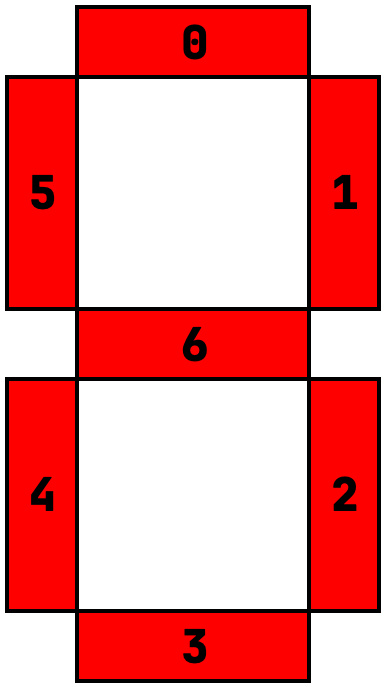
\includegraphics[width=0.3\textwidth]{Figures/Part1-7seg.jpg}
    \figcaption{7-segment display ports}
    \label{fig:T017seg}
\end{figure}

Then solving the boolean algebra I got the following result in table~\ref{tab:T01expression}. Formatting note: \verb|!| before a letter means logical \verb|NOT| and the operation only applies to the first letter directly after \verb|!|, letters beside each other means logical \verb|AND|, and \verb|+| means logical \verb|OR|. The expressions are always structured as SOP (Sum of products). \ref{Code:Part1_TLE.vhd}

% Table generated by Excel2LaTeX from sheet 'Part1'
\begin{table}[htbp]
  \centering
  \caption{Minimized solutions}
    \begin{tabular}{|c|c|}
    \hline
    HEX   & Expression \bigstrut\\
    \hline
    0     & \cellcolor[rgb]{ .71,  .902,  .635}!a!b!cd + b!d \bigstrut\\
    \hline
    1     & \cellcolor[rgb]{ .71,  .902,  .635}b!cd + bc!d \bigstrut\\
    \hline
    2     & \cellcolor[rgb]{ .71,  .902,  .635}!bc!d \bigstrut\\
    \hline
    3     & \cellcolor[rgb]{ .71,  .902,  .635}!b!cd + b!c!d + bcd \bigstrut\\
    \hline
    4     & \cellcolor[rgb]{ .71,  .902,  .635}b!c + d \bigstrut\\
    \hline
    5     & \cellcolor[rgb]{ .71,  .902,  .635}!a!bd + !bc + cd \bigstrut\\
    \hline
    6     & \cellcolor[rgb]{ .71,  .902,  .635}!a!b!c + bcd \bigstrut\\
    \hline
    \end{tabular}%
  \label{tab:T01expression}%
\end{table}%

\clearpage
\subsection{Code}
\writecode[VHDL]{Part1_TLE.vhd}{TLE as described in the task}

\clearpage
\subsection{RTL}
\begin{figure}[h]
    \centering
    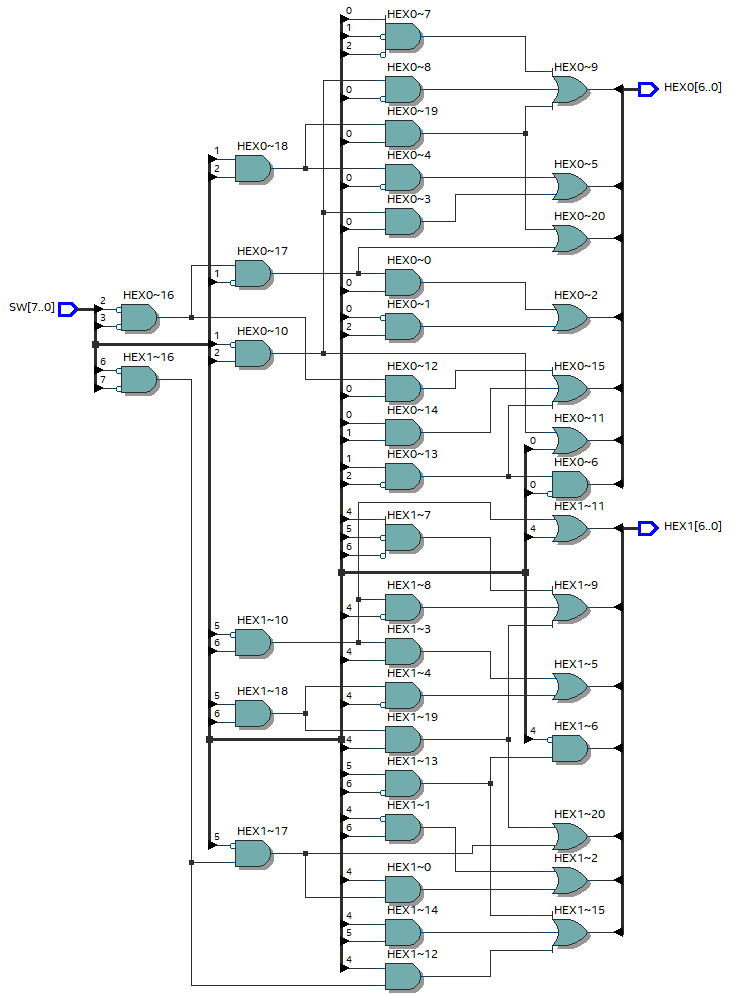
\includegraphics[width=0.85\textwidth]{Figures/Part1-RTL.jpg}
    \figcaption{RTL synthesizing of the TLE}
    \label{fig:T01rtl}
\end{figure}

\clearpage
\subsection{Results}
\begin{figure}[h]
    \centering
    \begin{subfigure}{0.4\textwidth}
        \centering
        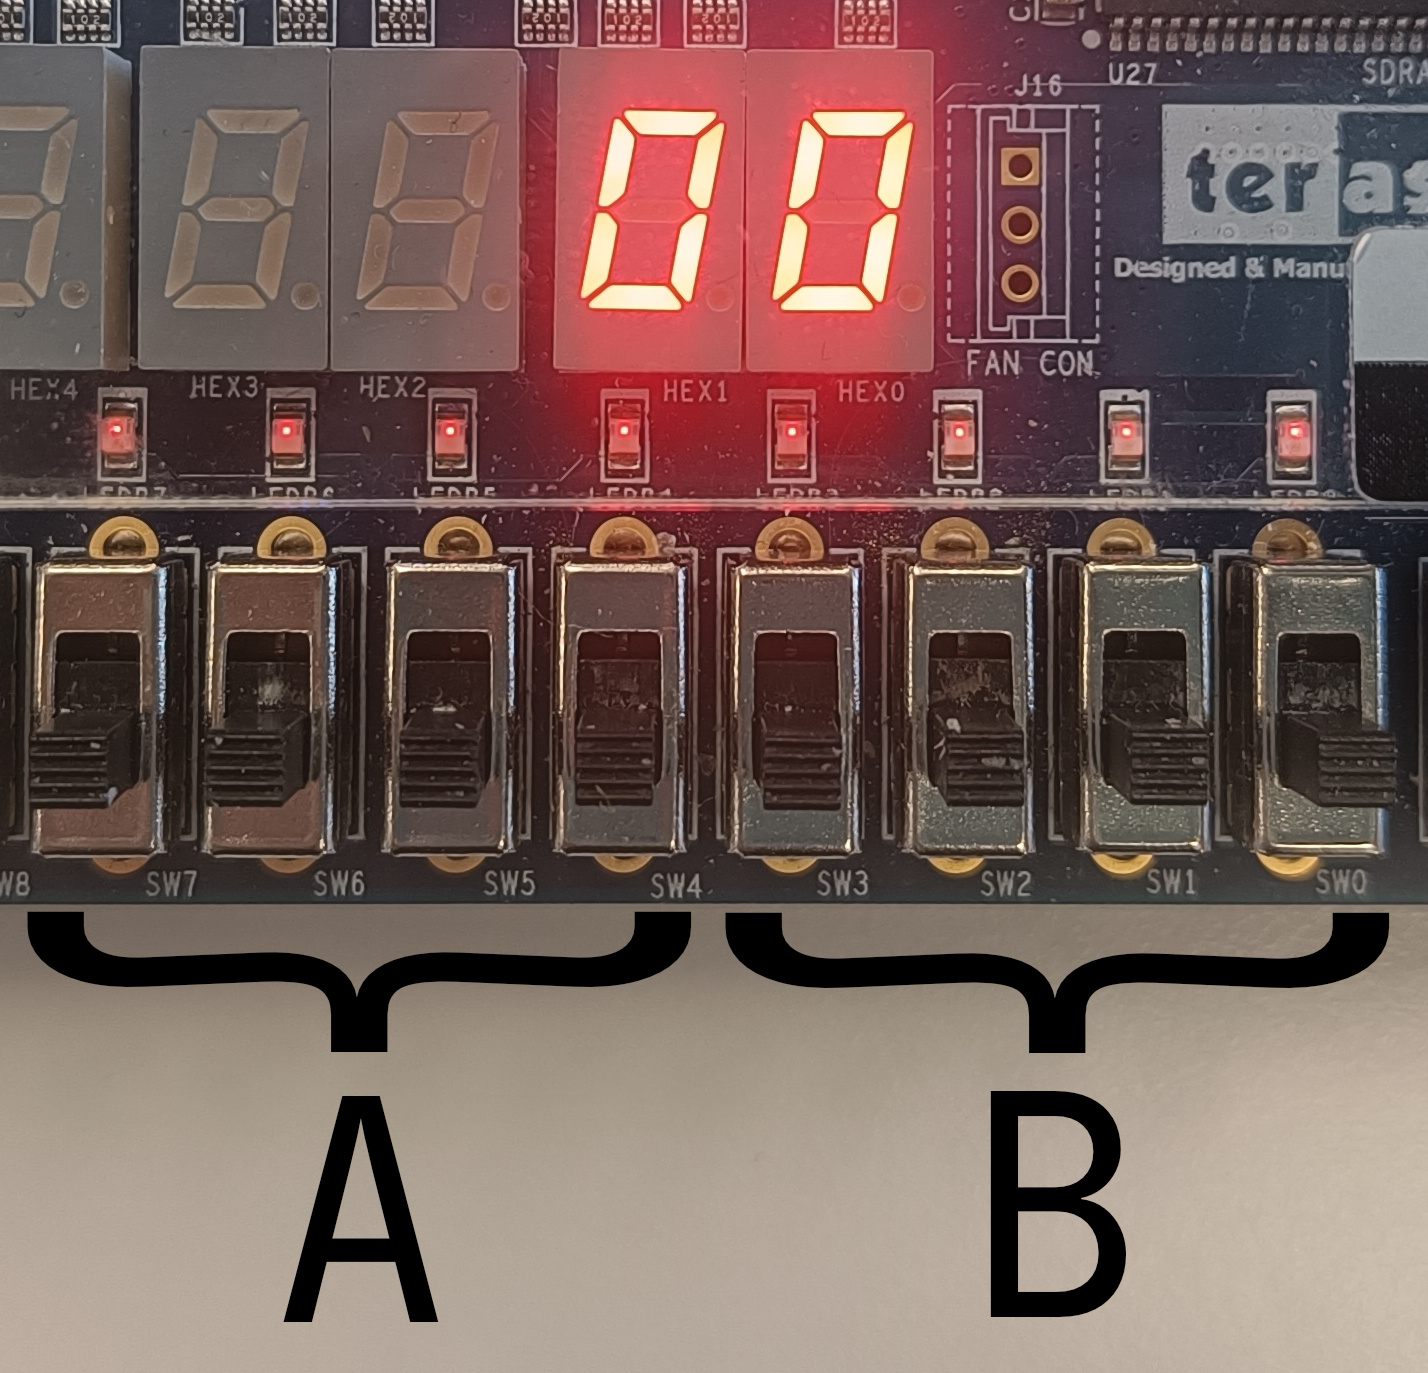
\includegraphics[width=1\textwidth]{Figures/Part1-0_0.jpg}
        \caption{BCD 0 0 as expected}
        \label{fig:T01pic1}
    \end{subfigure}
    \hfill
    \begin{subfigure}{0.4\textwidth}
        \centering
        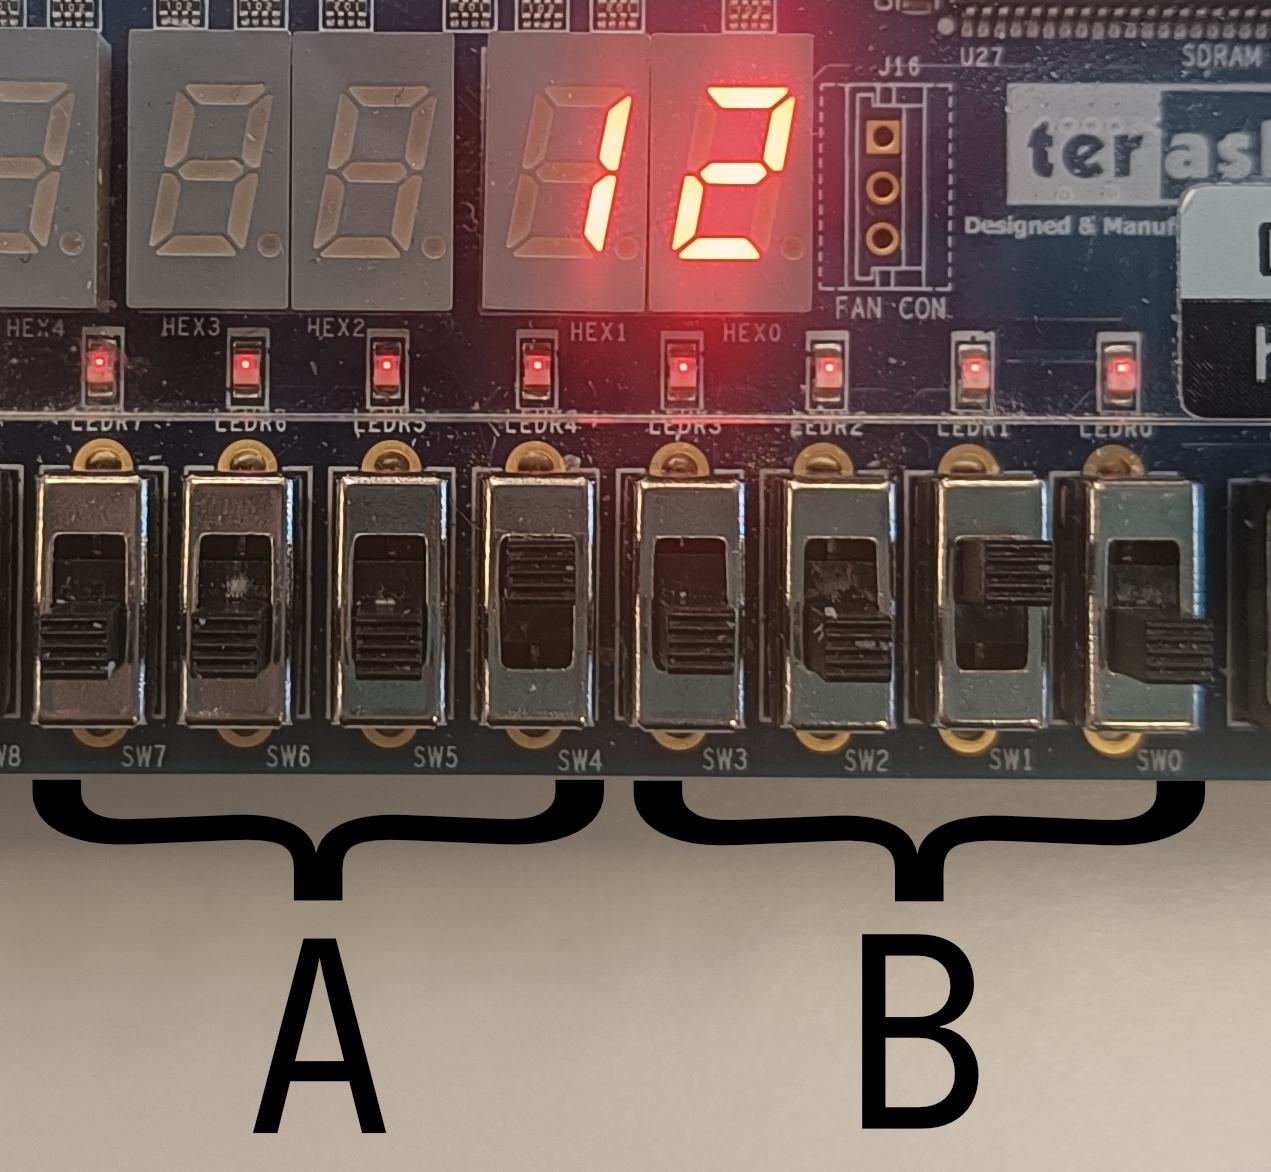
\includegraphics[width=1\textwidth]{Figures/Part1-1_2.jpg}
        \caption{BCD 1 2 as expected}
        \label{fig:T01pic2}
    \end{subfigure}
    \begin{subfigure}{0.4\textwidth}
        \centering
        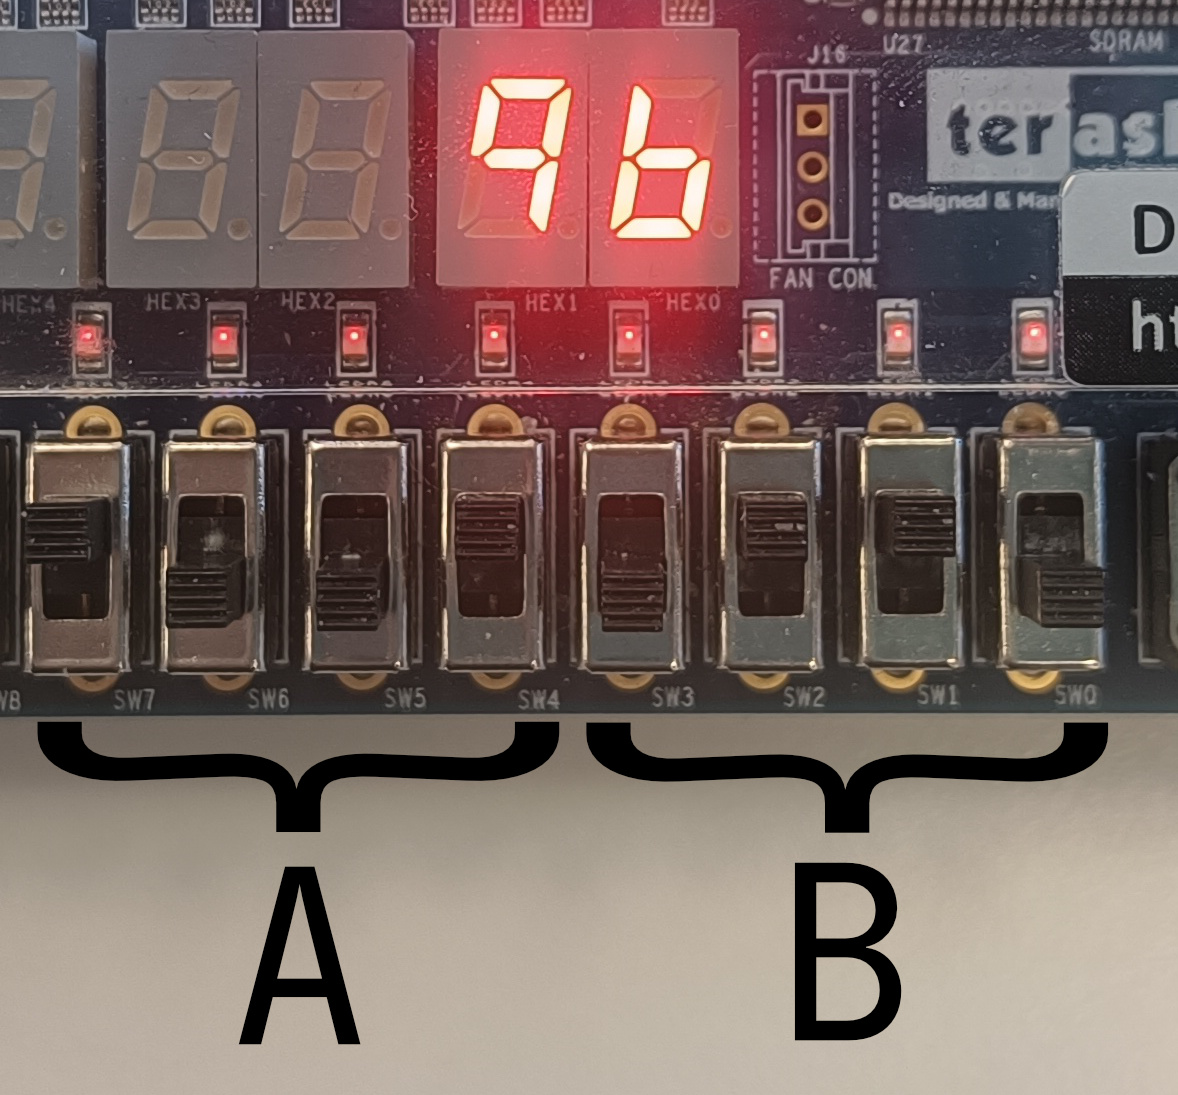
\includegraphics[width=1\textwidth]{Figures/Part1-9_6.jpg}
        \caption{BCD 9 6 as expected}
        \label{fig:T01pic3}
    \end{subfigure}
    \hfill
    \begin{subfigure}{0.4\textwidth}
        \centering
        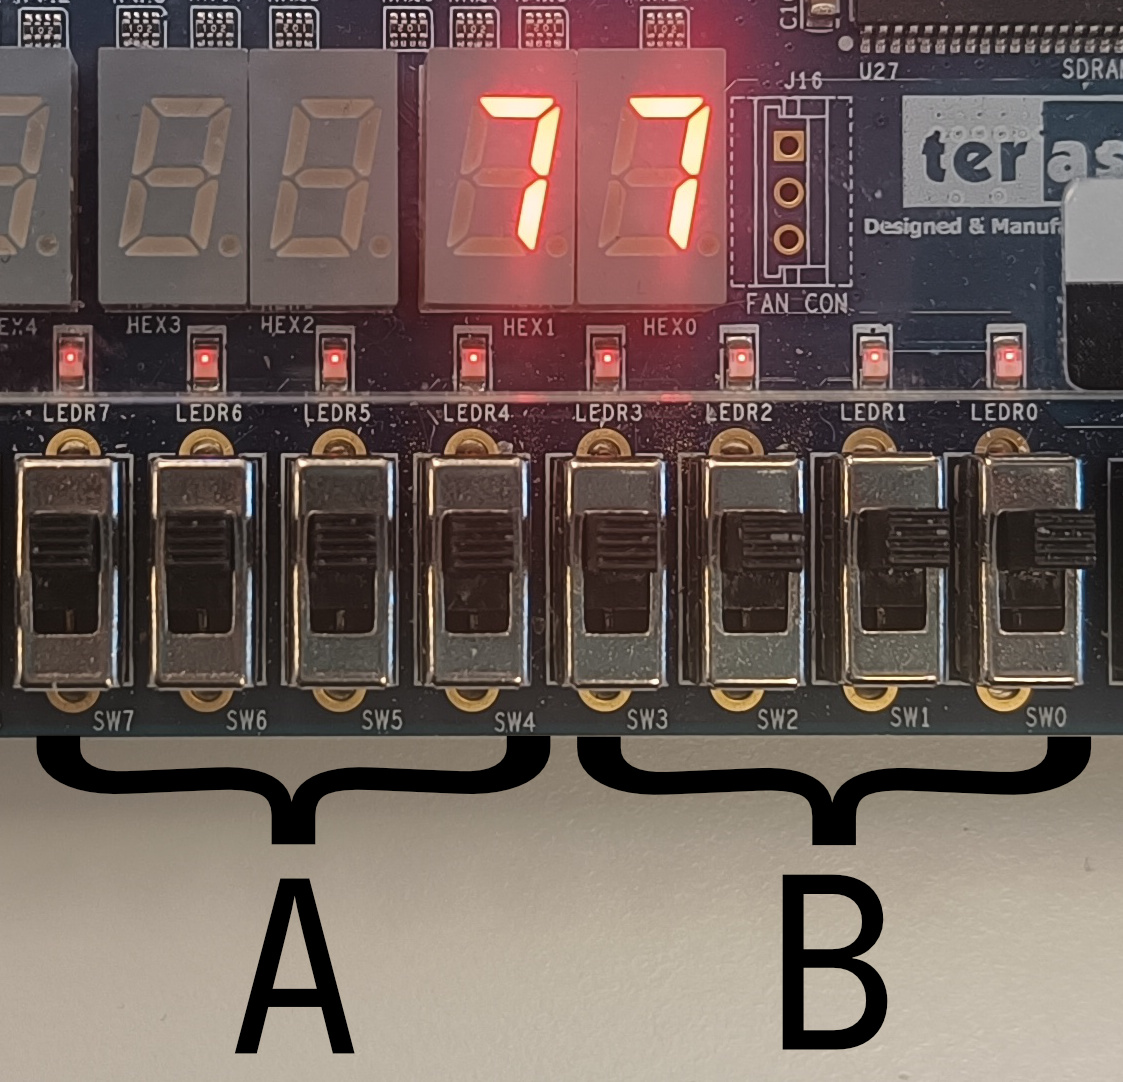
\includegraphics[width=1\textwidth]{Figures/Part1-15_15.jpg}
        \caption{Out of bounds result}
        \label{fig:T01pic4}
    \end{subfigure}
    \figcaption{Test results}
    \label{fig:T01pic}
\end{figure}


%   ############################## Section ##############################
\section{Part 2}
Expanding on the BCD values from part 1, part 2 is about making a 4 bit input BCD number to appear as a two digit decimal number. As the task suggests, this means making a comparator that checks whether above 9 or not and sets the 10´s digit to 1 if above and 0 if not. At the same time this comparator can signify when the 1´s digit should just display the current BCD value and when it should be modified with a multiplexer. When 9 or below, the BCD should be displayed as is, and when above 9 it should modify the input such that it starts from 0 and goes to 5 for the numbers 10 to 15, this is marked circuit A, both in the tasks diagram and in my comment.

\subsection{Solving}
I started with making table~\ref{tab:T02Z} and table~\ref{tab:T02A} using the mapping from table~\ref{tab:T02SW}.

% Table generated by Excel2LaTeX from sheet 'Part2'
\begin{table}[htbp]
  \centering
  \caption{Desired output from Z}
    \begin{tabular}{|c|c|c|c|c|c|c|c|c|}
    \hline
    \multirow{2}[4]{*}{NR} & \multicolumn{4}{c|}{SW}       & \multicolumn{4}{c|}{Z} \bigstrut\\
\cline{2-9}          & a     & b     & c     & d     & 3     & 2     & 1     & 0 \bigstrut\\
    \hline
    0     & \cellcolor[rgb]{ .851,  .851,  .851}0 & \cellcolor[rgb]{ .851,  .851,  .851}0 & \cellcolor[rgb]{ .851,  .851,  .851}0 & \cellcolor[rgb]{ .851,  .851,  .851}0 & \cellcolor[rgb]{ .71,  .902,  .635}0 & \cellcolor[rgb]{ .71,  .902,  .635}0 & \cellcolor[rgb]{ .71,  .902,  .635}0 & \cellcolor[rgb]{ .71,  .902,  .635}0 \bigstrut\\
    \hline
    1     & \cellcolor[rgb]{ .851,  .851,  .851}0 & \cellcolor[rgb]{ .851,  .851,  .851}0 & \cellcolor[rgb]{ .851,  .851,  .851}0 & \cellcolor[rgb]{ .851,  .851,  .851}1 & \cellcolor[rgb]{ .71,  .902,  .635}0 & \cellcolor[rgb]{ .71,  .902,  .635}0 & \cellcolor[rgb]{ .71,  .902,  .635}0 & \cellcolor[rgb]{ .71,  .902,  .635}0 \bigstrut\\
    \hline
    2     & \cellcolor[rgb]{ .851,  .851,  .851}0 & \cellcolor[rgb]{ .851,  .851,  .851}0 & \cellcolor[rgb]{ .851,  .851,  .851}1 & \cellcolor[rgb]{ .851,  .851,  .851}0 & \cellcolor[rgb]{ .71,  .902,  .635}0 & \cellcolor[rgb]{ .71,  .902,  .635}0 & \cellcolor[rgb]{ .71,  .902,  .635}0 & \cellcolor[rgb]{ .71,  .902,  .635}0 \bigstrut\\
    \hline
    3     & \cellcolor[rgb]{ .851,  .851,  .851}0 & \cellcolor[rgb]{ .851,  .851,  .851}0 & \cellcolor[rgb]{ .851,  .851,  .851}1 & \cellcolor[rgb]{ .851,  .851,  .851}1 & \cellcolor[rgb]{ .71,  .902,  .635}0 & \cellcolor[rgb]{ .71,  .902,  .635}0 & \cellcolor[rgb]{ .71,  .902,  .635}0 & \cellcolor[rgb]{ .71,  .902,  .635}0 \bigstrut\\
    \hline
    4     & \cellcolor[rgb]{ .851,  .851,  .851}0 & \cellcolor[rgb]{ .851,  .851,  .851}1 & \cellcolor[rgb]{ .851,  .851,  .851}0 & \cellcolor[rgb]{ .851,  .851,  .851}0 & \cellcolor[rgb]{ .71,  .902,  .635}0 & \cellcolor[rgb]{ .71,  .902,  .635}0 & \cellcolor[rgb]{ .71,  .902,  .635}0 & \cellcolor[rgb]{ .71,  .902,  .635}0 \bigstrut\\
    \hline
    5     & \cellcolor[rgb]{ .851,  .851,  .851}0 & \cellcolor[rgb]{ .851,  .851,  .851}1 & \cellcolor[rgb]{ .851,  .851,  .851}0 & \cellcolor[rgb]{ .851,  .851,  .851}1 & \cellcolor[rgb]{ .71,  .902,  .635}0 & \cellcolor[rgb]{ .71,  .902,  .635}0 & \cellcolor[rgb]{ .71,  .902,  .635}0 & \cellcolor[rgb]{ .71,  .902,  .635}0 \bigstrut\\
    \hline
    6     & \cellcolor[rgb]{ .851,  .851,  .851}0 & \cellcolor[rgb]{ .851,  .851,  .851}1 & \cellcolor[rgb]{ .851,  .851,  .851}1 & \cellcolor[rgb]{ .851,  .851,  .851}0 & \cellcolor[rgb]{ .71,  .902,  .635}0 & \cellcolor[rgb]{ .71,  .902,  .635}0 & \cellcolor[rgb]{ .71,  .902,  .635}0 & \cellcolor[rgb]{ .71,  .902,  .635}0 \bigstrut\\
    \hline
    7     & \cellcolor[rgb]{ .851,  .851,  .851}0 & \cellcolor[rgb]{ .851,  .851,  .851}1 & \cellcolor[rgb]{ .851,  .851,  .851}1 & \cellcolor[rgb]{ .851,  .851,  .851}1 & \cellcolor[rgb]{ .71,  .902,  .635}0 & \cellcolor[rgb]{ .71,  .902,  .635}0 & \cellcolor[rgb]{ .71,  .902,  .635}0 & \cellcolor[rgb]{ .71,  .902,  .635}0 \bigstrut\\
    \hline
    8     & \cellcolor[rgb]{ .851,  .851,  .851}1 & \cellcolor[rgb]{ .851,  .851,  .851}0 & \cellcolor[rgb]{ .851,  .851,  .851}0 & \cellcolor[rgb]{ .851,  .851,  .851}0 & \cellcolor[rgb]{ .71,  .902,  .635}0 & \cellcolor[rgb]{ .71,  .902,  .635}0 & \cellcolor[rgb]{ .71,  .902,  .635}0 & \cellcolor[rgb]{ .71,  .902,  .635}0 \bigstrut\\
    \hline
    9     & \cellcolor[rgb]{ .851,  .851,  .851}1 & \cellcolor[rgb]{ .851,  .851,  .851}0 & \cellcolor[rgb]{ .851,  .851,  .851}0 & \cellcolor[rgb]{ .851,  .851,  .851}1 & \cellcolor[rgb]{ .71,  .902,  .635}0 & \cellcolor[rgb]{ .71,  .902,  .635}0 & \cellcolor[rgb]{ .71,  .902,  .635}0 & \cellcolor[rgb]{ .71,  .902,  .635}0 \bigstrut\\
    \hline
    10    & \cellcolor[rgb]{ .851,  .851,  .851}1 & \cellcolor[rgb]{ .851,  .851,  .851}0 & \cellcolor[rgb]{ .851,  .851,  .851}1 & \cellcolor[rgb]{ .851,  .851,  .851}0 & \cellcolor[rgb]{ .71,  .902,  .635}0 & \cellcolor[rgb]{ .71,  .902,  .635}0 & \cellcolor[rgb]{ .71,  .902,  .635}0 & \cellcolor[rgb]{ .71,  .902,  .635}1 \bigstrut\\
    \hline
    11    & \cellcolor[rgb]{ .851,  .851,  .851}1 & \cellcolor[rgb]{ .851,  .851,  .851}0 & \cellcolor[rgb]{ .851,  .851,  .851}1 & \cellcolor[rgb]{ .851,  .851,  .851}1 & \cellcolor[rgb]{ .71,  .902,  .635}0 & \cellcolor[rgb]{ .71,  .902,  .635}0 & \cellcolor[rgb]{ .71,  .902,  .635}0 & \cellcolor[rgb]{ .71,  .902,  .635}1 \bigstrut\\
    \hline
    12    & \cellcolor[rgb]{ .851,  .851,  .851}1 & \cellcolor[rgb]{ .851,  .851,  .851}1 & \cellcolor[rgb]{ .851,  .851,  .851}0 & \cellcolor[rgb]{ .851,  .851,  .851}0 & \cellcolor[rgb]{ .71,  .902,  .635}0 & \cellcolor[rgb]{ .71,  .902,  .635}0 & \cellcolor[rgb]{ .71,  .902,  .635}0 & \cellcolor[rgb]{ .71,  .902,  .635}1 \bigstrut\\
    \hline
    13    & \cellcolor[rgb]{ .851,  .851,  .851}1 & \cellcolor[rgb]{ .851,  .851,  .851}1 & \cellcolor[rgb]{ .851,  .851,  .851}0 & \cellcolor[rgb]{ .851,  .851,  .851}1 & \cellcolor[rgb]{ .71,  .902,  .635}0 & \cellcolor[rgb]{ .71,  .902,  .635}0 & \cellcolor[rgb]{ .71,  .902,  .635}0 & \cellcolor[rgb]{ .71,  .902,  .635}1 \bigstrut\\
    \hline
    14    & \cellcolor[rgb]{ .851,  .851,  .851}1 & \cellcolor[rgb]{ .851,  .851,  .851}1 & \cellcolor[rgb]{ .851,  .851,  .851}1 & \cellcolor[rgb]{ .851,  .851,  .851}0 & \cellcolor[rgb]{ .71,  .902,  .635}0 & \cellcolor[rgb]{ .71,  .902,  .635}0 & \cellcolor[rgb]{ .71,  .902,  .635}0 & \cellcolor[rgb]{ .71,  .902,  .635}1 \bigstrut\\
    \hline
    15    & \cellcolor[rgb]{ .851,  .851,  .851}1 & \cellcolor[rgb]{ .851,  .851,  .851}1 & \cellcolor[rgb]{ .851,  .851,  .851}1 & \cellcolor[rgb]{ .851,  .851,  .851}1 & \cellcolor[rgb]{ .71,  .902,  .635}0 & \cellcolor[rgb]{ .71,  .902,  .635}0 & \cellcolor[rgb]{ .71,  .902,  .635}0 & \cellcolor[rgb]{ .71,  .902,  .635}1 \bigstrut\\
    \hline
    \end{tabular}%
  \label{tab:T02Z}%
\end{table}%

\clearpage
% Table generated by Excel2LaTeX from sheet 'Part2'
\begin{table}[htbp]
  \centering
  \caption{Desired output from A}
    \begin{tabular}{|c|c|c|c|c|c|c|c|c|}
    \hline
    \multirow{2}[4]{*}{NR} & \multicolumn{4}{c|}{SW}       & \multicolumn{4}{c|}{A} \bigstrut\\
\cline{2-9}          & a     & b     & c     & d     & 3     & 2     & 1     & 0 \bigstrut\\
    \hline
    0     & \cellcolor[rgb]{ .851,  .851,  .851}0 & \cellcolor[rgb]{ .851,  .851,  .851}0 & \cellcolor[rgb]{ .851,  .851,  .851}0 & \cellcolor[rgb]{ .851,  .851,  .851}0 & \cellcolor[rgb]{ .969,  .78,  .675}* & \cellcolor[rgb]{ .969,  .78,  .675}* & \cellcolor[rgb]{ .969,  .78,  .675}* & \cellcolor[rgb]{ .969,  .78,  .675}* \bigstrut\\
    \hline
    1     & \cellcolor[rgb]{ .851,  .851,  .851}0 & \cellcolor[rgb]{ .851,  .851,  .851}0 & \cellcolor[rgb]{ .851,  .851,  .851}0 & \cellcolor[rgb]{ .851,  .851,  .851}1 & \cellcolor[rgb]{ .969,  .78,  .675}* & \cellcolor[rgb]{ .969,  .78,  .675}* & \cellcolor[rgb]{ .969,  .78,  .675}* & \cellcolor[rgb]{ .969,  .78,  .675}* \bigstrut\\
    \hline
    2     & \cellcolor[rgb]{ .851,  .851,  .851}0 & \cellcolor[rgb]{ .851,  .851,  .851}0 & \cellcolor[rgb]{ .851,  .851,  .851}1 & \cellcolor[rgb]{ .851,  .851,  .851}0 & \cellcolor[rgb]{ .969,  .78,  .675}* & \cellcolor[rgb]{ .969,  .78,  .675}* & \cellcolor[rgb]{ .969,  .78,  .675}* & \cellcolor[rgb]{ .969,  .78,  .675}* \bigstrut\\
    \hline
    3     & \cellcolor[rgb]{ .851,  .851,  .851}0 & \cellcolor[rgb]{ .851,  .851,  .851}0 & \cellcolor[rgb]{ .851,  .851,  .851}1 & \cellcolor[rgb]{ .851,  .851,  .851}1 & \cellcolor[rgb]{ .969,  .78,  .675}* & \cellcolor[rgb]{ .969,  .78,  .675}* & \cellcolor[rgb]{ .969,  .78,  .675}* & \cellcolor[rgb]{ .969,  .78,  .675}* \bigstrut\\
    \hline
    4     & \cellcolor[rgb]{ .851,  .851,  .851}0 & \cellcolor[rgb]{ .851,  .851,  .851}1 & \cellcolor[rgb]{ .851,  .851,  .851}0 & \cellcolor[rgb]{ .851,  .851,  .851}0 & \cellcolor[rgb]{ .969,  .78,  .675}* & \cellcolor[rgb]{ .969,  .78,  .675}* & \cellcolor[rgb]{ .969,  .78,  .675}* & \cellcolor[rgb]{ .969,  .78,  .675}* \bigstrut\\
    \hline
    5     & \cellcolor[rgb]{ .851,  .851,  .851}0 & \cellcolor[rgb]{ .851,  .851,  .851}1 & \cellcolor[rgb]{ .851,  .851,  .851}0 & \cellcolor[rgb]{ .851,  .851,  .851}1 & \cellcolor[rgb]{ .969,  .78,  .675}* & \cellcolor[rgb]{ .969,  .78,  .675}* & \cellcolor[rgb]{ .969,  .78,  .675}* & \cellcolor[rgb]{ .969,  .78,  .675}* \bigstrut\\
    \hline
    6     & \cellcolor[rgb]{ .851,  .851,  .851}0 & \cellcolor[rgb]{ .851,  .851,  .851}1 & \cellcolor[rgb]{ .851,  .851,  .851}1 & \cellcolor[rgb]{ .851,  .851,  .851}0 & \cellcolor[rgb]{ .969,  .78,  .675}* & \cellcolor[rgb]{ .969,  .78,  .675}* & \cellcolor[rgb]{ .969,  .78,  .675}* & \cellcolor[rgb]{ .969,  .78,  .675}* \bigstrut\\
    \hline
    7     & \cellcolor[rgb]{ .851,  .851,  .851}0 & \cellcolor[rgb]{ .851,  .851,  .851}1 & \cellcolor[rgb]{ .851,  .851,  .851}1 & \cellcolor[rgb]{ .851,  .851,  .851}1 & \cellcolor[rgb]{ .969,  .78,  .675}* & \cellcolor[rgb]{ .969,  .78,  .675}* & \cellcolor[rgb]{ .969,  .78,  .675}* & \cellcolor[rgb]{ .969,  .78,  .675}* \bigstrut\\
    \hline
    8     & \cellcolor[rgb]{ .851,  .851,  .851}1 & \cellcolor[rgb]{ .851,  .851,  .851}0 & \cellcolor[rgb]{ .851,  .851,  .851}0 & \cellcolor[rgb]{ .851,  .851,  .851}0 & \cellcolor[rgb]{ .969,  .78,  .675}* & \cellcolor[rgb]{ .969,  .78,  .675}* & \cellcolor[rgb]{ .969,  .78,  .675}* & \cellcolor[rgb]{ .969,  .78,  .675}* \bigstrut\\
    \hline
    9     & \cellcolor[rgb]{ .851,  .851,  .851}1 & \cellcolor[rgb]{ .851,  .851,  .851}0 & \cellcolor[rgb]{ .851,  .851,  .851}0 & \cellcolor[rgb]{ .851,  .851,  .851}1 & \cellcolor[rgb]{ .969,  .78,  .675}* & \cellcolor[rgb]{ .969,  .78,  .675}* & \cellcolor[rgb]{ .969,  .78,  .675}* & \cellcolor[rgb]{ .969,  .78,  .675}* \bigstrut\\
    \hline
    10    & \cellcolor[rgb]{ .851,  .851,  .851}1 & \cellcolor[rgb]{ .851,  .851,  .851}0 & \cellcolor[rgb]{ .851,  .851,  .851}1 & \cellcolor[rgb]{ .851,  .851,  .851}0 & \cellcolor[rgb]{ .71,  .902,  .635}0 & \cellcolor[rgb]{ .71,  .902,  .635}0 & \cellcolor[rgb]{ .71,  .902,  .635}0 & \cellcolor[rgb]{ .71,  .902,  .635}0 \bigstrut\\
    \hline
    11    & \cellcolor[rgb]{ .851,  .851,  .851}1 & \cellcolor[rgb]{ .851,  .851,  .851}0 & \cellcolor[rgb]{ .851,  .851,  .851}1 & \cellcolor[rgb]{ .851,  .851,  .851}1 & \cellcolor[rgb]{ .71,  .902,  .635}0 & \cellcolor[rgb]{ .71,  .902,  .635}0 & \cellcolor[rgb]{ .71,  .902,  .635}0 & \cellcolor[rgb]{ .71,  .902,  .635}1 \bigstrut\\
    \hline
    12    & \cellcolor[rgb]{ .851,  .851,  .851}1 & \cellcolor[rgb]{ .851,  .851,  .851}1 & \cellcolor[rgb]{ .851,  .851,  .851}0 & \cellcolor[rgb]{ .851,  .851,  .851}0 & \cellcolor[rgb]{ .71,  .902,  .635}0 & \cellcolor[rgb]{ .71,  .902,  .635}0 & \cellcolor[rgb]{ .71,  .902,  .635}1 & \cellcolor[rgb]{ .71,  .902,  .635}0 \bigstrut\\
    \hline
    13    & \cellcolor[rgb]{ .851,  .851,  .851}1 & \cellcolor[rgb]{ .851,  .851,  .851}1 & \cellcolor[rgb]{ .851,  .851,  .851}0 & \cellcolor[rgb]{ .851,  .851,  .851}1 & \cellcolor[rgb]{ .71,  .902,  .635}0 & \cellcolor[rgb]{ .71,  .902,  .635}0 & \cellcolor[rgb]{ .71,  .902,  .635}1 & \cellcolor[rgb]{ .71,  .902,  .635}1 \bigstrut\\
    \hline
    14    & \cellcolor[rgb]{ .851,  .851,  .851}1 & \cellcolor[rgb]{ .851,  .851,  .851}1 & \cellcolor[rgb]{ .851,  .851,  .851}1 & \cellcolor[rgb]{ .851,  .851,  .851}0 & \cellcolor[rgb]{ .71,  .902,  .635}0 & \cellcolor[rgb]{ .71,  .902,  .635}1 & \cellcolor[rgb]{ .71,  .902,  .635}0 & \cellcolor[rgb]{ .71,  .902,  .635}0 \bigstrut\\
    \hline
    15    & \cellcolor[rgb]{ .851,  .851,  .851}1 & \cellcolor[rgb]{ .851,  .851,  .851}1 & \cellcolor[rgb]{ .851,  .851,  .851}1 & \cellcolor[rgb]{ .851,  .851,  .851}1 & \cellcolor[rgb]{ .71,  .902,  .635}0 & \cellcolor[rgb]{ .71,  .902,  .635}1 & \cellcolor[rgb]{ .71,  .902,  .635}0 & \cellcolor[rgb]{ .71,  .902,  .635}1 \bigstrut\\
    \hline
    \end{tabular}%
  \label{tab:T02A}%
\end{table}%

% Table generated by Excel2LaTeX from sheet 'Part2'
\begin{table}[htbp]
  \centering
  \caption{Switch mapping}
    \begin{tabular}{|c|c|}
    \hline
    a     & SW(3) \bigstrut\\
    \hline
    b     & SW(2) \bigstrut\\
    \hline
    c     & SW(1) \bigstrut\\
    \hline
    d     & SW(0) \bigstrut\\
    \hline
    \end{tabular}%
  \label{tab:T02SW}%
\end{table}%

\clearpage
Solving the boolean algebra, I found the following expressions.

% Table generated by Excel2LaTeX from sheet 'Part2'
\begin{table}[htbp]
  \centering
  \caption{Minimized solutions for Z}
    \begin{tabular}{|c|c|}
    \hline
    Z     & Expression \bigstrut\\
    \hline
    0     & \cellcolor[rgb]{ .71,  .902,  .635}ac + ab \bigstrut\\
    \hline
    1     & \cellcolor[rgb]{ .71,  .902,  .635}0 \bigstrut\\
    \hline
    2     & \cellcolor[rgb]{ .71,  .902,  .635}0 \bigstrut\\
    \hline
    3     & \cellcolor[rgb]{ .71,  .902,  .635}0 \bigstrut\\
    \hline
    \end{tabular}%
  \label{tab:T02Zexpressions}%
\end{table}%

% Table generated by Excel2LaTeX from sheet 'Part2'
\begin{table}[htbp]
  \centering
  \caption{Minimized solutions for A}
    \begin{tabular}{|c|c|}
    \hline
    A     & Expression \bigstrut\\
    \hline
    0     & \cellcolor[rgb]{ .71,  .902,  .635}d \bigstrut\\
    \hline
    1     & \cellcolor[rgb]{ .71,  .902,  .635}!c \bigstrut\\
    \hline
    2     & \cellcolor[rgb]{ .71,  .902,  .635}bc \bigstrut\\
    \hline
    3     & \cellcolor[rgb]{ .71,  .902,  .635}0 \bigstrut\\
    \hline
    \end{tabular}%
  \label{tab:T02Aexpressions}%
\end{table}%

\clearpage
\subsection{Code}
\writecode[VHDL]{Part2_TLE.vhd}{TLE as described in the task}
\clearpage
\writecode[VHDL]{Part2_mux.vhd}{Multiplexer used in TLE}
\clearpage
\writecode[VHDL]{Part2_decoder.vhd}{7-seg decoder used in TLE}

\clearpage
\subsection{RTL}
\begin{figure}[h]
    \centering
    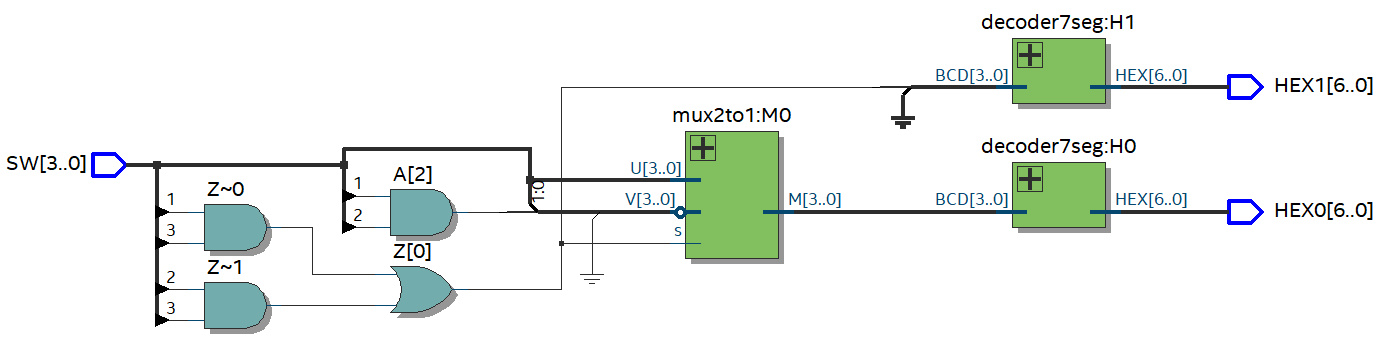
\includegraphics[width=1\textwidth]{Figures/Part2-RTL_TLE.jpg}
    \figcaption{RTL synthesizing of the TLE}
    \label{fig:T02rtl_tle}
\end{figure}
\begin{figure}[h]
    \centering
    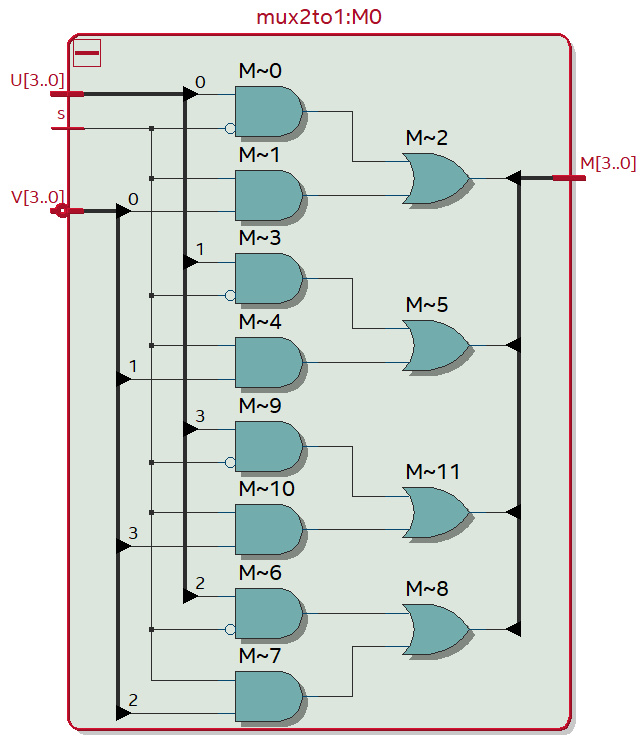
\includegraphics[width=0.6\textwidth]{Figures/Part2-RTL_mux.jpg}
    \figcaption{RTL synthesizing of the multiplexer}
    \label{fig:T02rtl_mux}
\end{figure}
\clearpage
\begin{figure}[h]
    \centering
    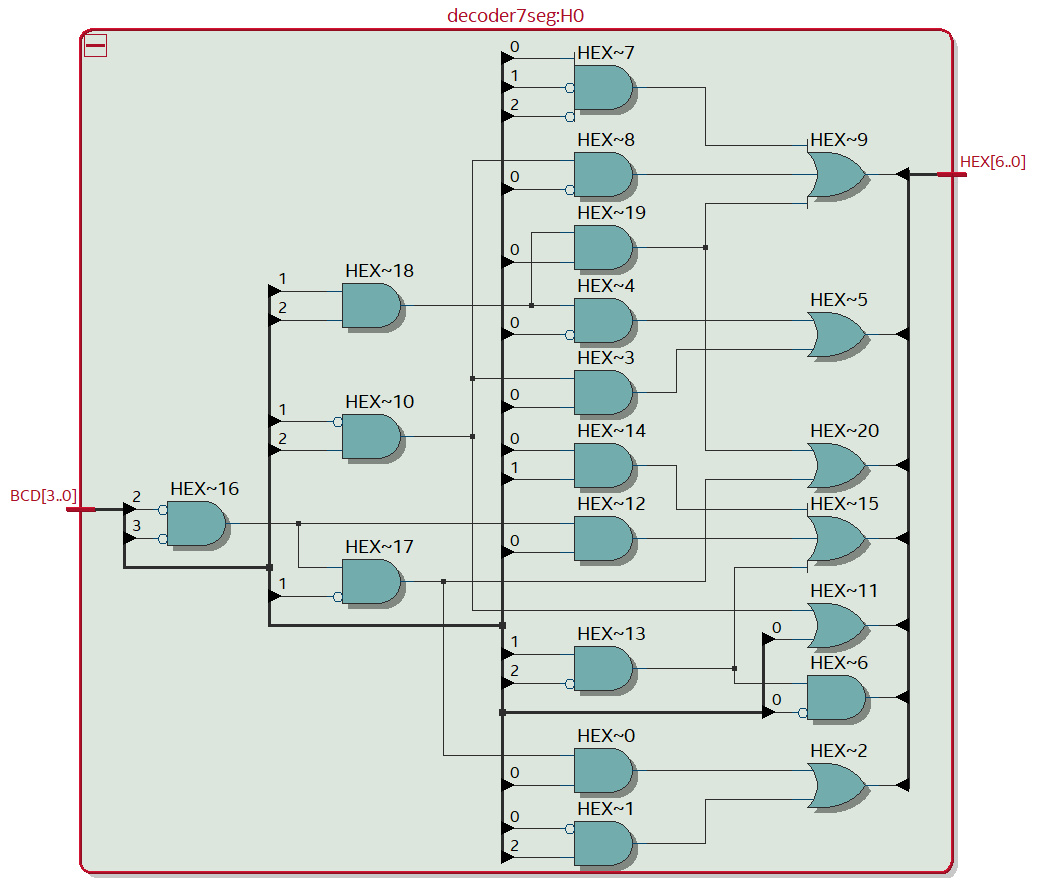
\includegraphics[width=1\textwidth]{Figures/Part2-RTL_decoder.jpg}
    \figcaption{RTL synthesizing of the 7-seg decoder}
    \label{fig:T02rtl_decoder}
\end{figure}

\clearpage
\subsection{Results}
\begin{figure}[h]
    \centering
    \begin{subfigure}{0.4\textwidth}
        \centering
        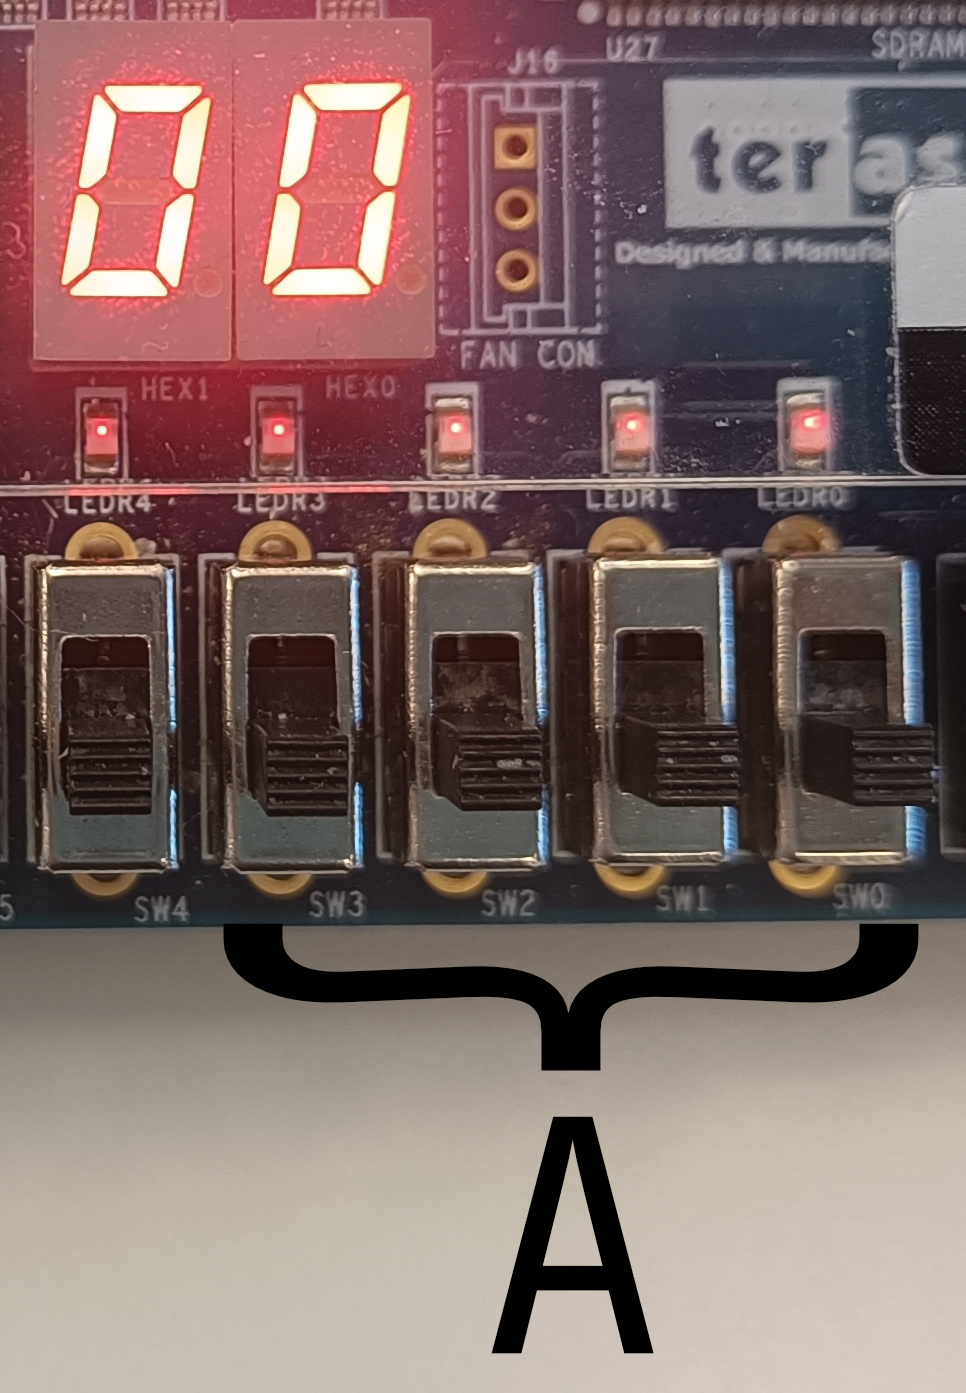
\includegraphics[width=0.8\textwidth]{Figures/Part2-0.jpg}
        \caption{BCD 0 as expected}
        \label{fig:T02pic1}
    \end{subfigure}
    \hfill
    \begin{subfigure}{0.4\textwidth}
        \centering
        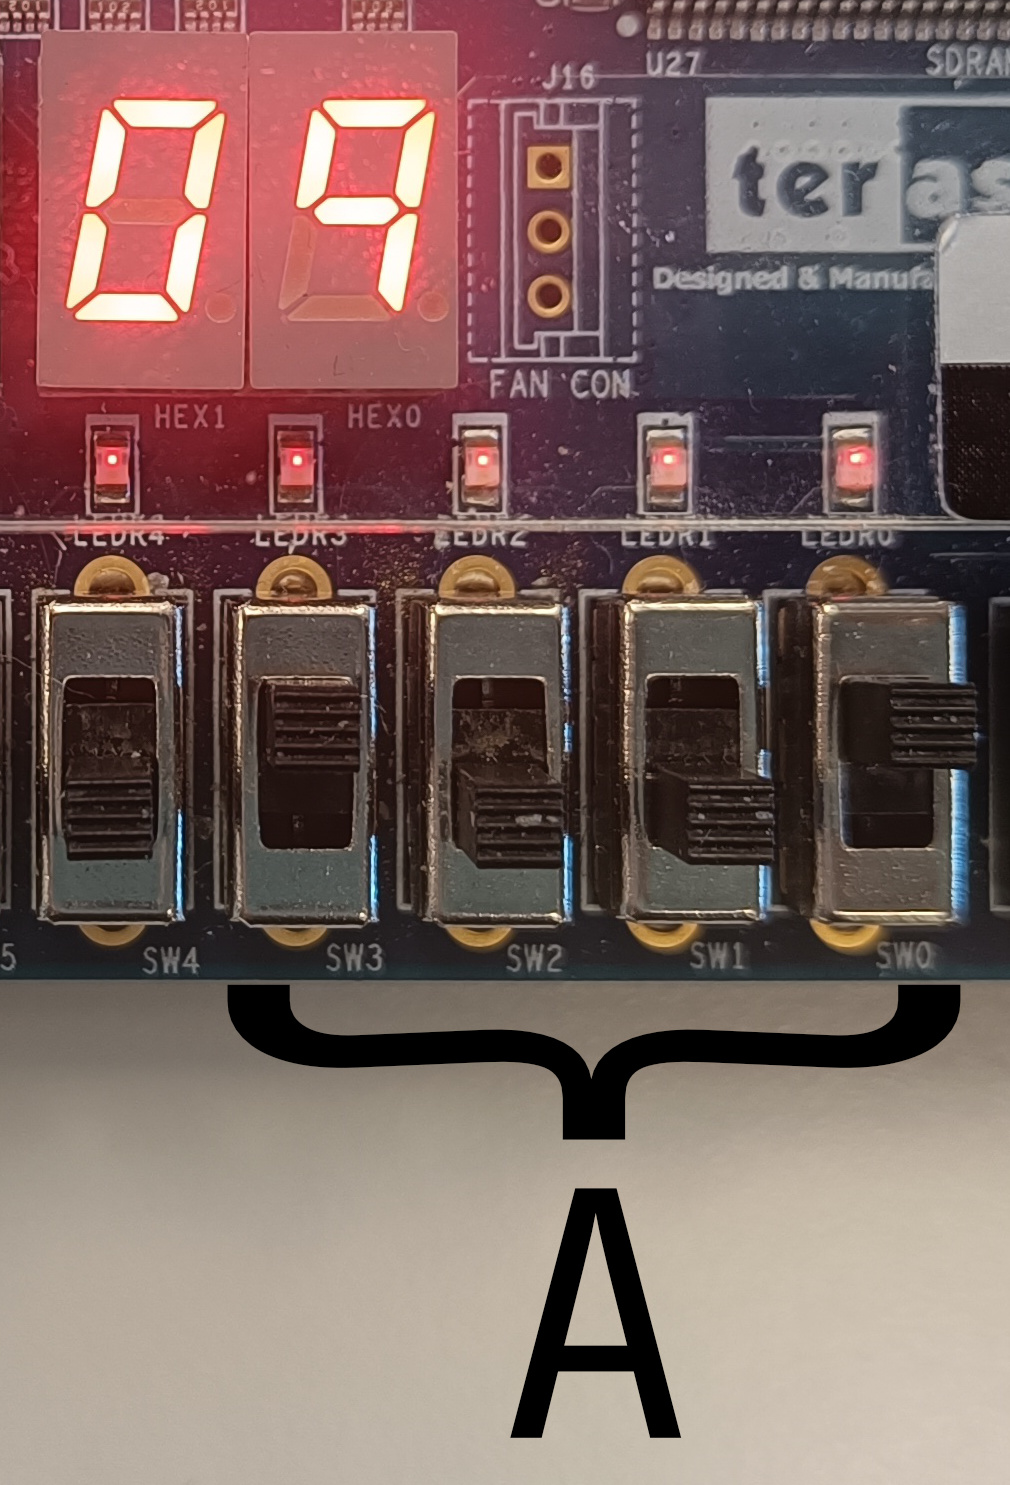
\includegraphics[width=0.8\textwidth]{Figures/Part2-9.jpg}
        \caption{BCD 9 as expected}
        \label{fig:T02pic2}
    \end{subfigure}
    \begin{subfigure}{0.4\textwidth}
        \centering
        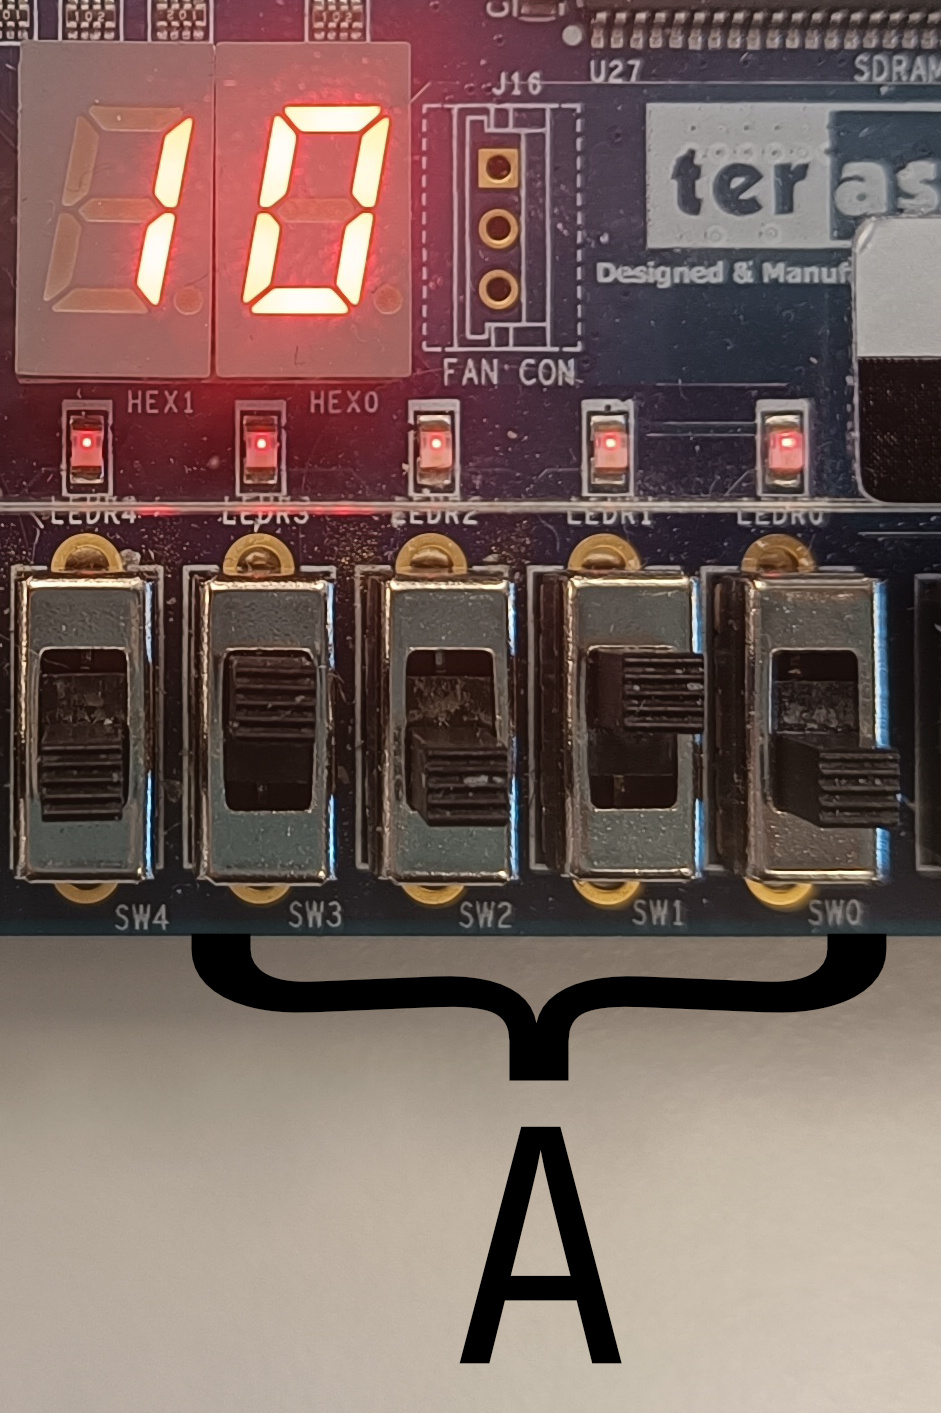
\includegraphics[width=0.8\textwidth]{Figures/Part2-10.jpg}
        \caption{BCD 10 as expected}
        \label{fig:T02pic3}
    \end{subfigure}
    \hfill
    \begin{subfigure}{0.4\textwidth}
        \centering
        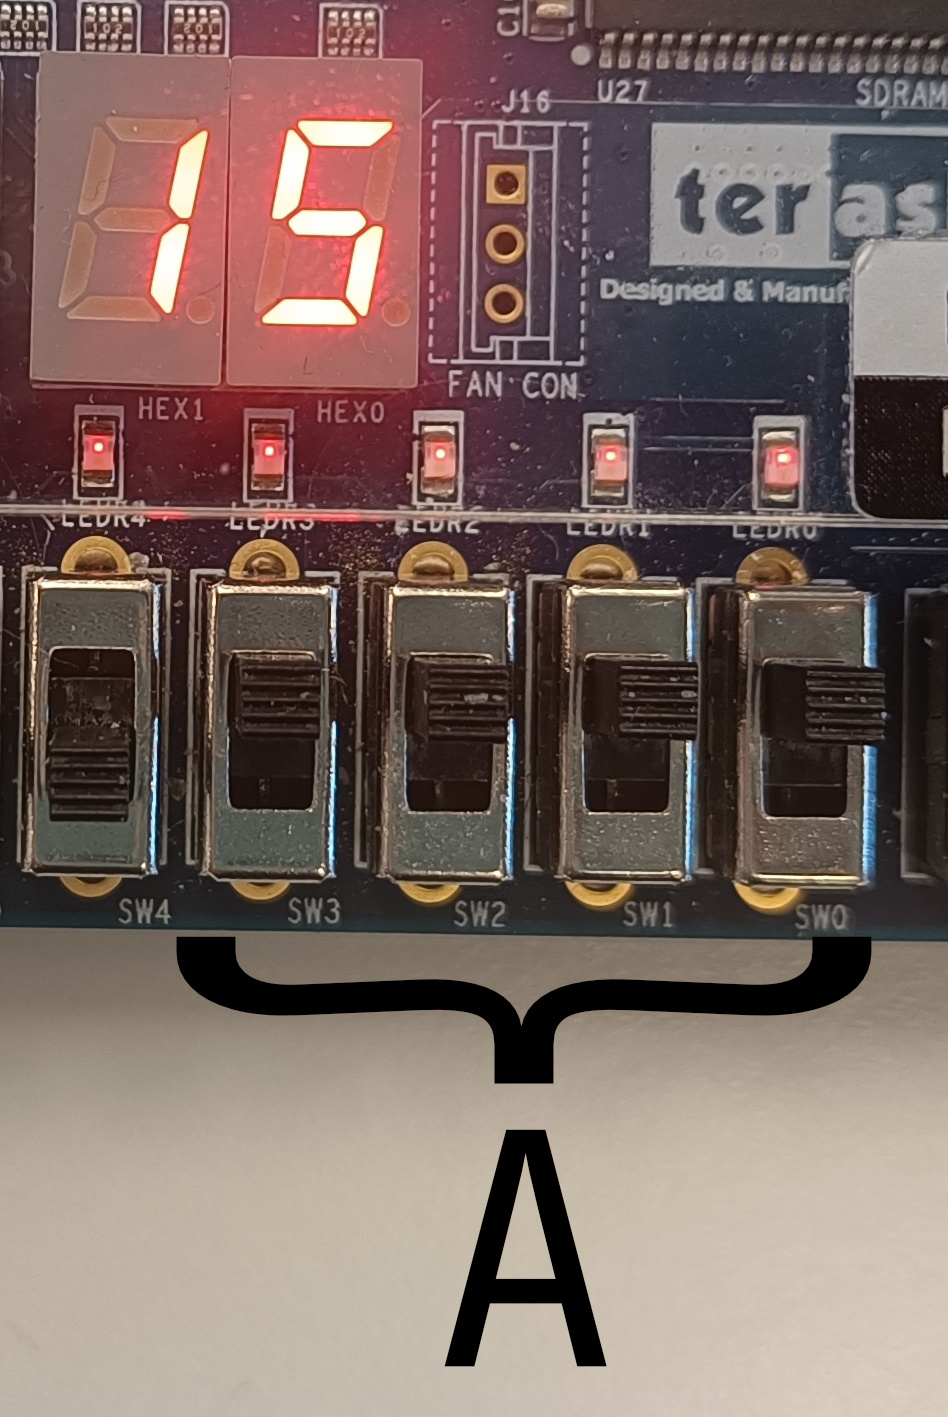
\includegraphics[width=0.8\textwidth]{Figures/Part2-15.jpg}
        \caption{BCD 15 as expected}
        \label{fig:T02pic4}
    \end{subfigure}
    \figcaption{Test results}
    \label{fig:T02pic}
\end{figure}


%   ############################## Section ##############################
\section{Part 3}
This parts is currently unrelated to the two previous parts as here we are making a 4-bit adder using 4 instances of a single bit adder. This task was probably designed to teach the use of multiple instances and how to import other code snippets using components. As I already have done that multiple times for readability and reusability this was a very simple task.

\subsection{Solving}
As opposed to the previous tasks, this time I used the provided table~\ref{tab:T03addertruthtable} for the single bit adder and found the expressions shown in table~\ref{tab:T03expression}.

% Table generated by Excel2LaTeX from sheet 'Part3'
\begin{table}[htbp]
  \centering
  \caption{Provided table for adder}
    \begin{tabular}{|c|c|c|c|c|}
    \hline
    \multicolumn{3}{|c|}{In} & \multicolumn{2}{c|}{Out} \bigstrut\\
    \hline
    Ci    & B     & A     & Co    & S \bigstrut\\
    \hline
    \rowcolor[rgb]{ .851,  .851,  .851} 0     & 0     & 0     & \cellcolor[rgb]{ .71,  .902,  .635}0 & \cellcolor[rgb]{ .71,  .902,  .635}0 \bigstrut\\
    \hline
    \rowcolor[rgb]{ .851,  .851,  .851} 0     & 0     & 1     & \cellcolor[rgb]{ .71,  .902,  .635}0 & \cellcolor[rgb]{ .71,  .902,  .635}1 \bigstrut\\
    \hline
    \rowcolor[rgb]{ .851,  .851,  .851} 0     & 1     & 0     & \cellcolor[rgb]{ .71,  .902,  .635}0 & \cellcolor[rgb]{ .71,  .902,  .635}1 \bigstrut\\
    \hline
    \rowcolor[rgb]{ .851,  .851,  .851} 0     & 1     & 1     & \cellcolor[rgb]{ .71,  .902,  .635}1 & \cellcolor[rgb]{ .71,  .902,  .635}0 \bigstrut\\
    \hline
    \rowcolor[rgb]{ .851,  .851,  .851} 1     & 0     & 0     & \cellcolor[rgb]{ .71,  .902,  .635}0 & \cellcolor[rgb]{ .71,  .902,  .635}1 \bigstrut\\
    \hline
    \rowcolor[rgb]{ .851,  .851,  .851} 1     & 0     & 1     & \cellcolor[rgb]{ .71,  .902,  .635}1 & \cellcolor[rgb]{ .71,  .902,  .635}0 \bigstrut\\
    \hline
    \rowcolor[rgb]{ .851,  .851,  .851} 1     & 1     & 0     & \cellcolor[rgb]{ .71,  .902,  .635}1 & \cellcolor[rgb]{ .71,  .902,  .635}0 \bigstrut\\
    \hline
    \rowcolor[rgb]{ .851,  .851,  .851} 1     & 1     & 1     & \cellcolor[rgb]{ .71,  .902,  .635}1 & \cellcolor[rgb]{ .71,  .902,  .635}1 \bigstrut\\
    \hline
    \end{tabular}%
  \label{tab:T03addertruthtable}%
\end{table}%

% Table generated by Excel2LaTeX from sheet 'Part3'
\begin{table}[htbp]
  \centering
  \caption{Minimized solutions}
    \begin{tabular}{|c|c|}
    \hline
    Out   & Expression \bigstrut\\
    \hline
    S     & \cellcolor[rgb]{ .71,  .902,  .635}!Ci!BA + !CiB!A + Ci!B!A + CiBA \bigstrut\\
    \hline
    Co    & \cellcolor[rgb]{ .71,  .902,  .635}BA + CiA + CiB \bigstrut\\
    \hline
    \end{tabular}%
  \label{tab:T03expression}%
\end{table}%

\clearpage
\subsection{Code}
\writecode[VHDL]{Part3_TLE.vhd}{TLE as described in the task}
\writecode[VHDL]{Part3_adder.vhd}{Single bit adder used in TLE}

\clearpage
\subsection{RTL}
\begin{figure}[h]
    \centering
    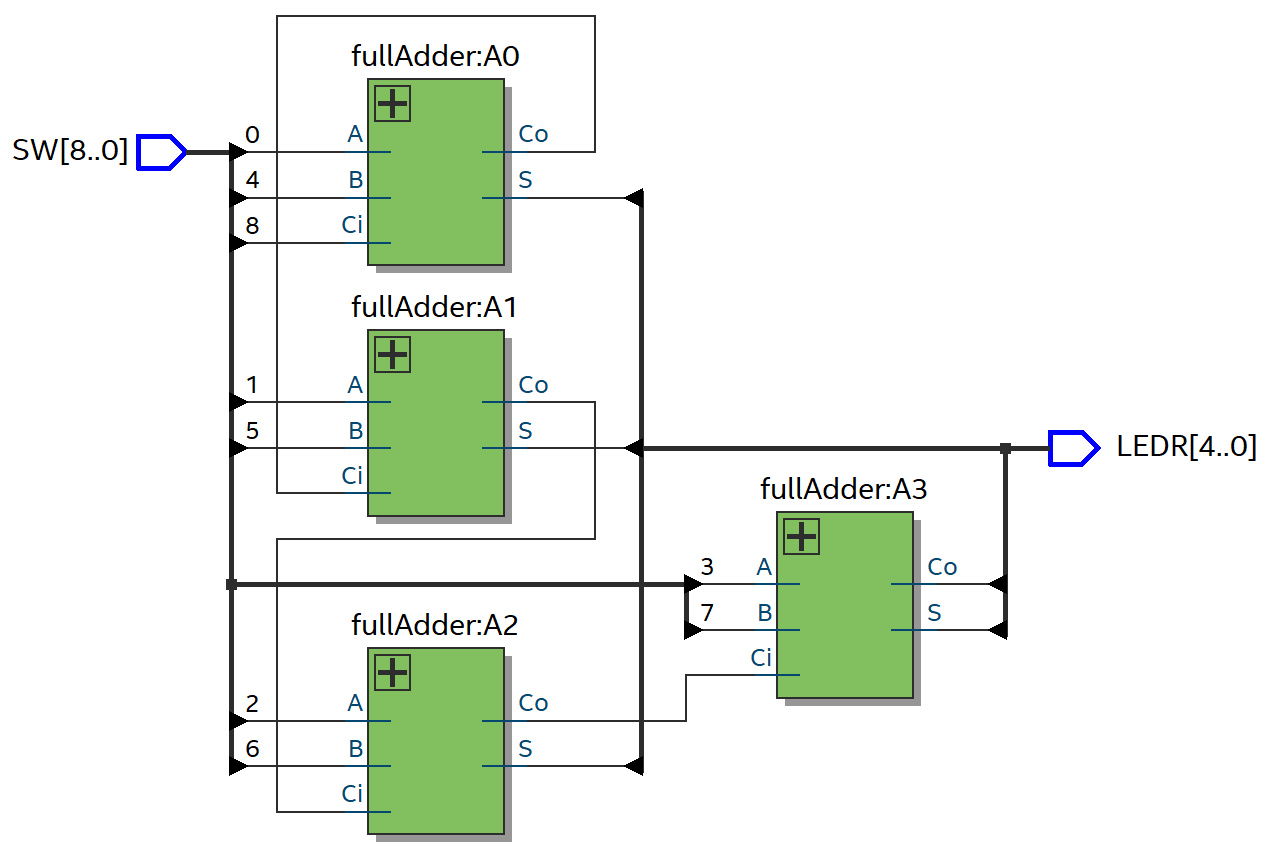
\includegraphics[width=1\textwidth]{Figures/Part3-RTL_TLE.jpg}
    \figcaption{RTL synthesizing of the TLE}
    \label{fig:T03rtl_tle}
\end{figure}
\clearpage
\begin{figure}[h]
    \centering
    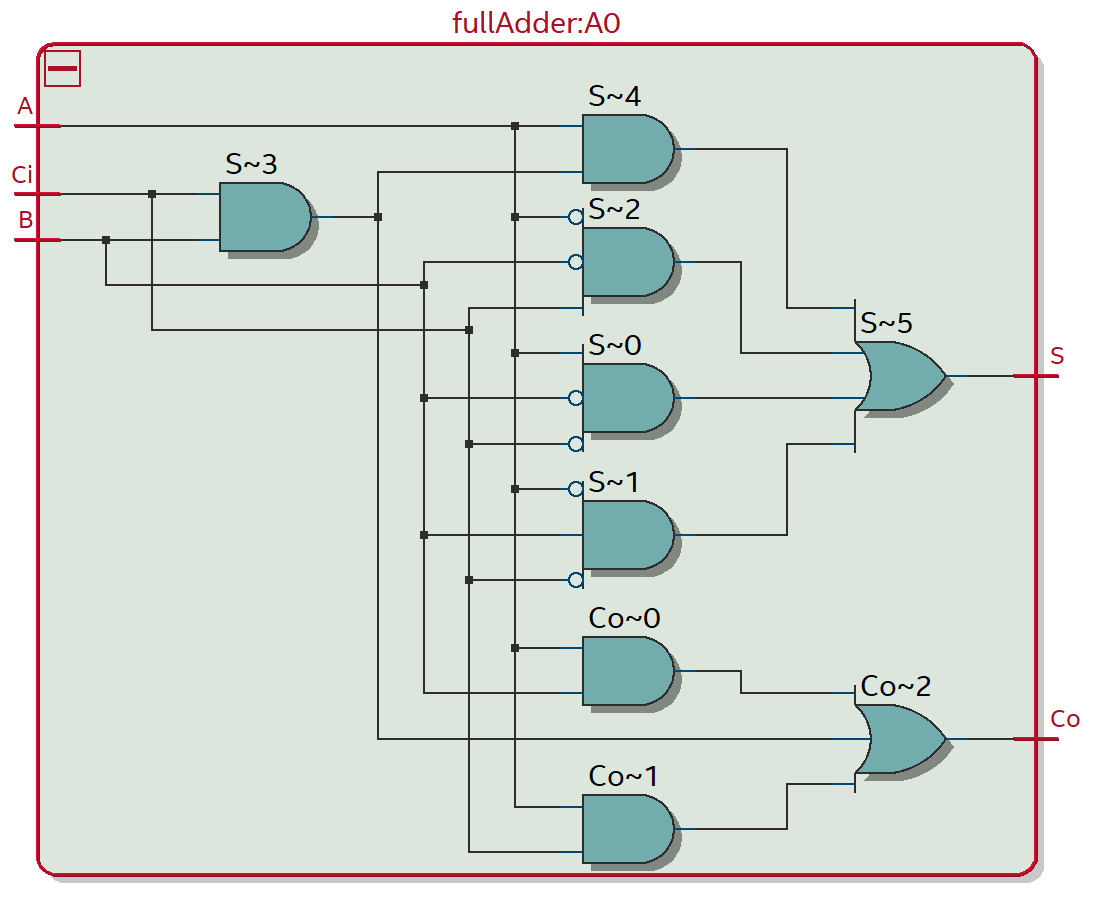
\includegraphics[width=1\textwidth]{Figures/Part3-RTL_adder.jpg}
    \figcaption{RTL synthesizing of a single bit adder instance}
    \label{fig:T03rtl_adder}
\end{figure}

\clearpage
\subsection{Results}
\begin{figure}[h]
    \centering
    \begin{subfigure}{0.4\textwidth}
        \centering
        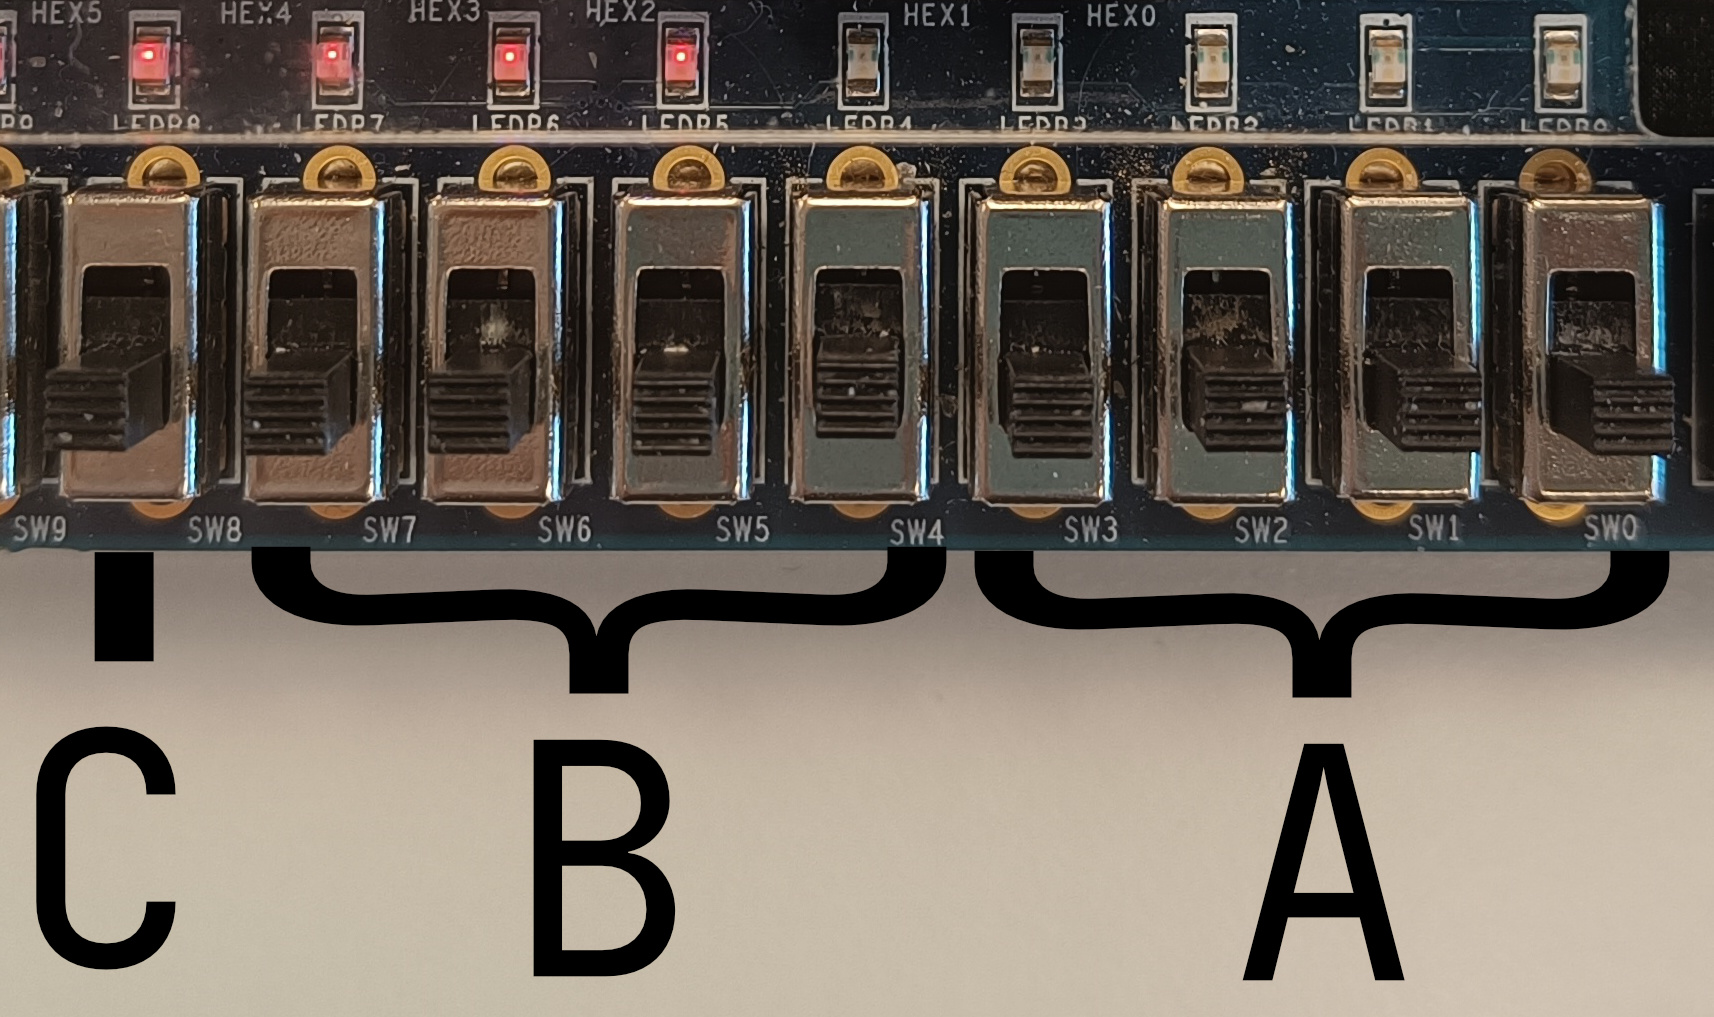
\includegraphics[width=1\textwidth]{Figures/Part3-0_0_0.jpg}
        \caption{0 + 0 + 0 = 0}
        \label{fig:T03pic1}
    \end{subfigure}
    \hfill
    \begin{subfigure}{0.4\textwidth}
        \centering
        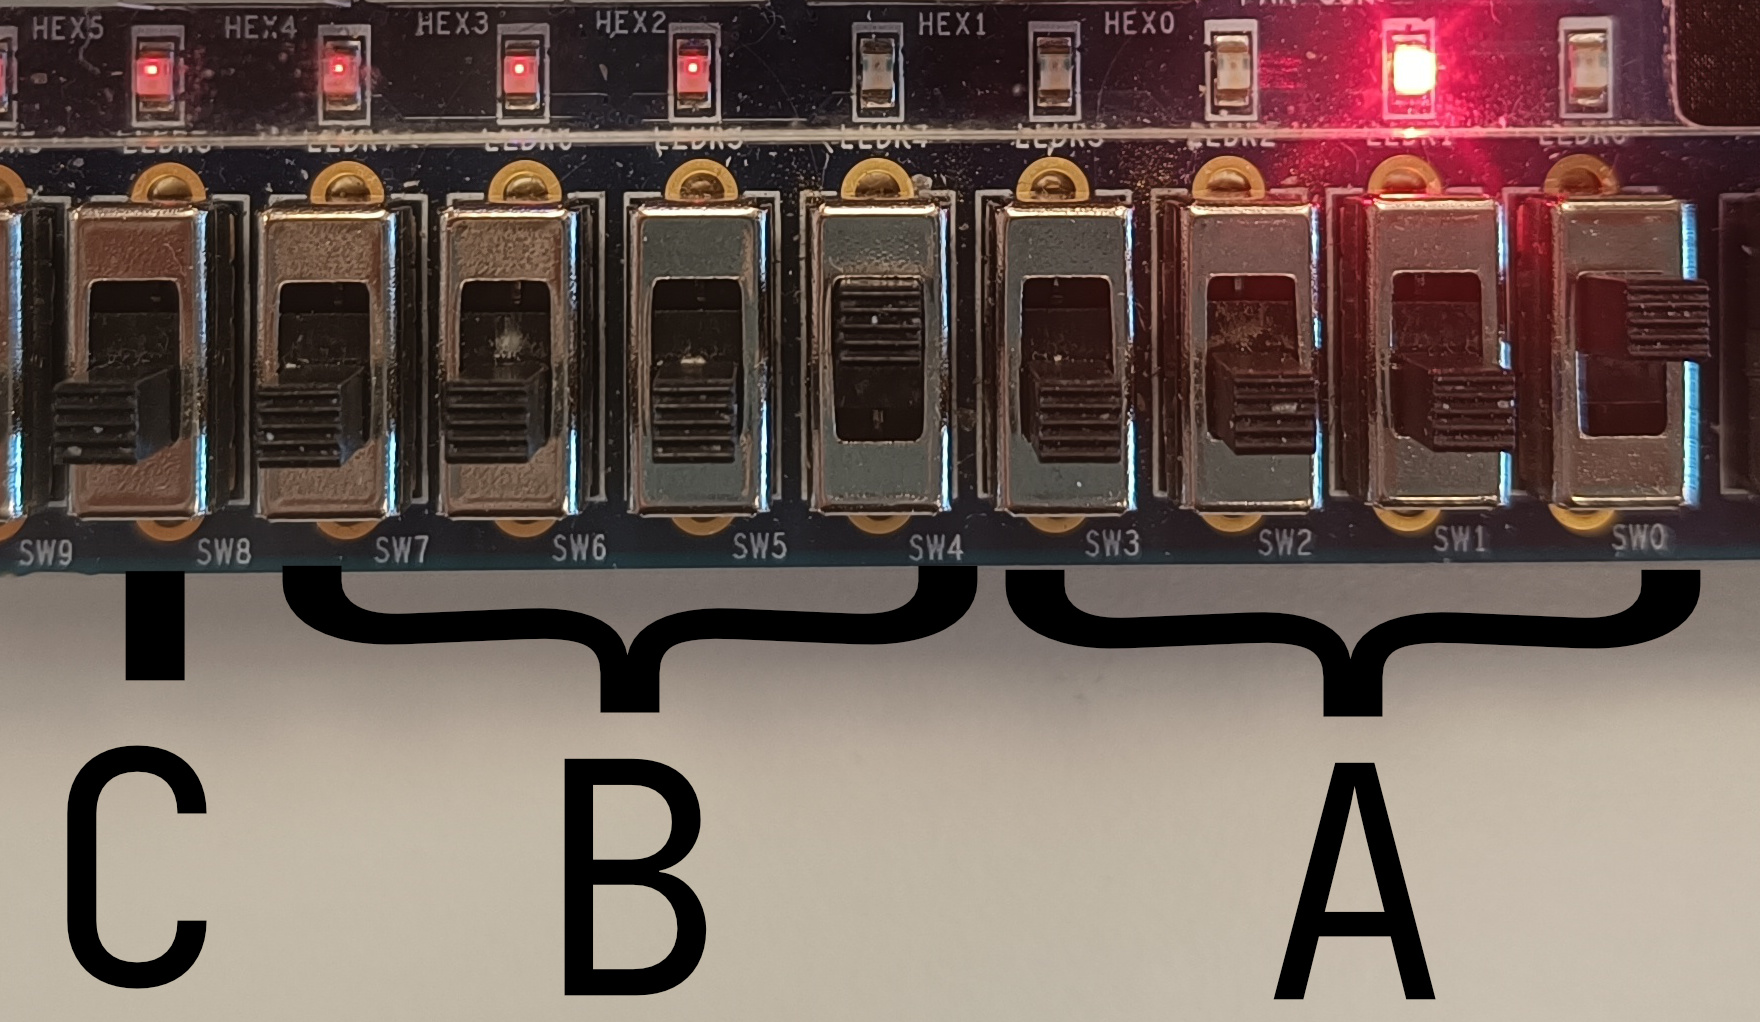
\includegraphics[width=1\textwidth]{Figures/Part3-0_1_1.jpg}
        \caption{0 + 1 + 1 = 2}
        \label{fig:T03pic2}
    \end{subfigure}
    \begin{subfigure}{0.4\textwidth}
        \centering
        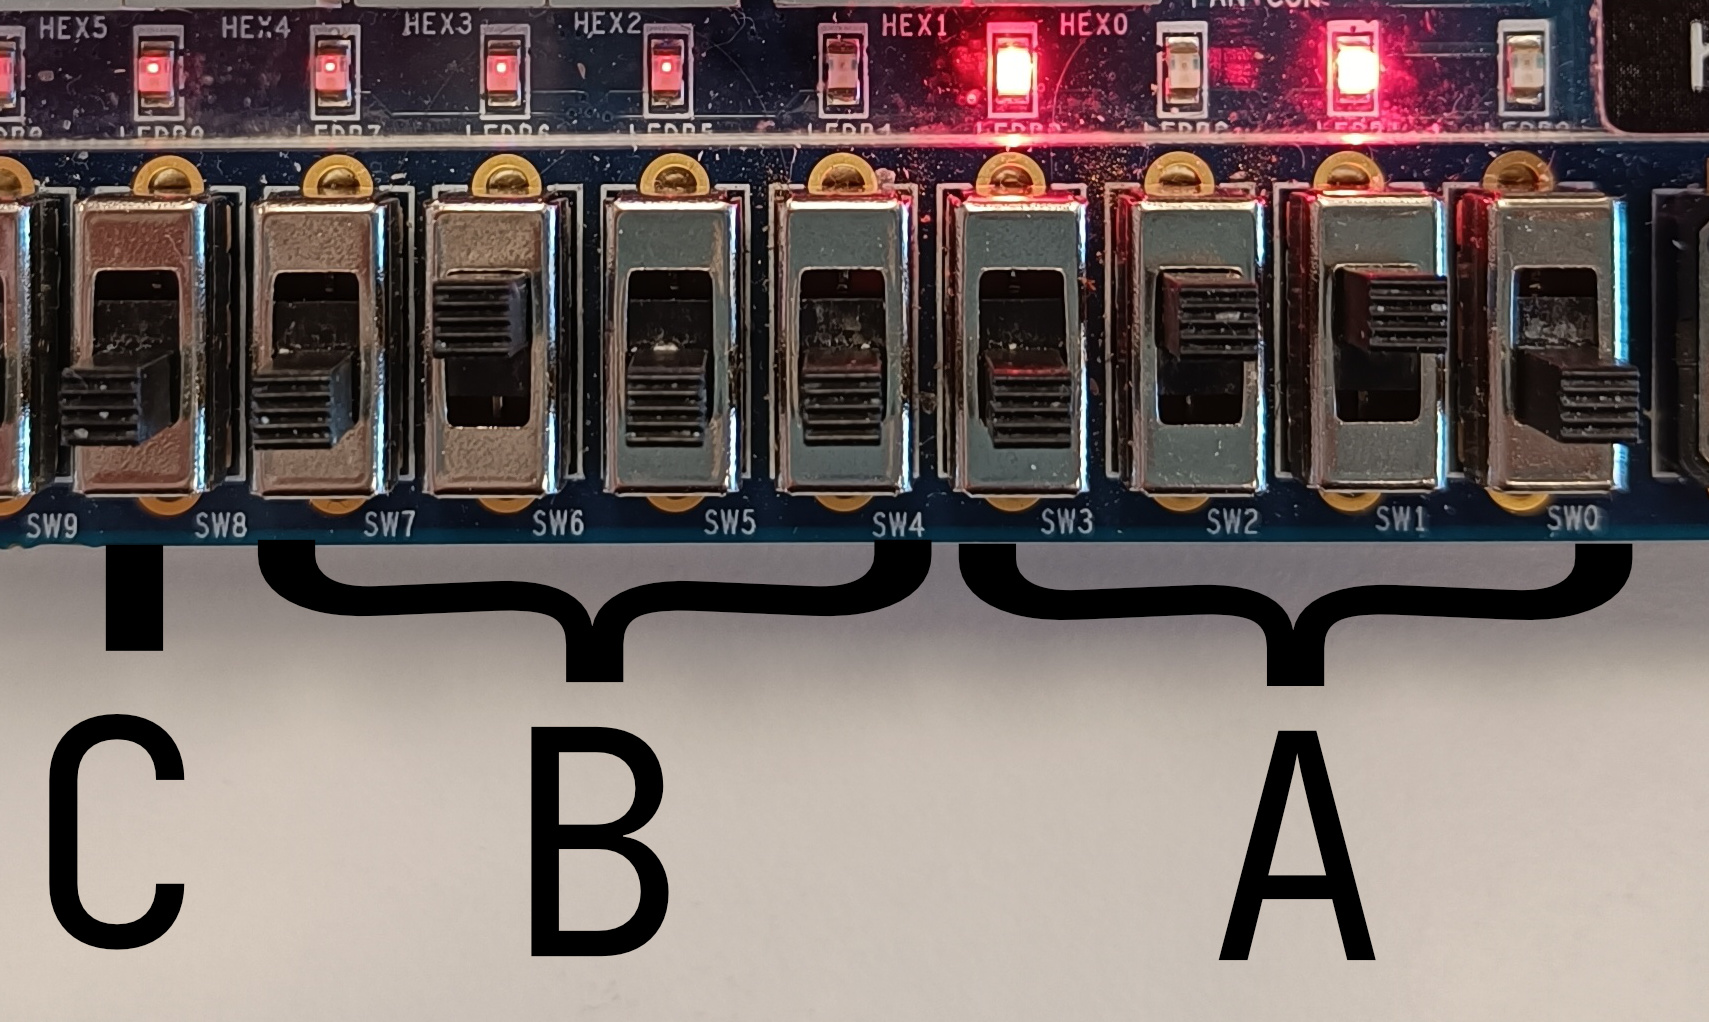
\includegraphics[width=1\textwidth]{Figures/Part3-0_4_6.jpg}
        \caption{0 + 4 + 6 = 10}
        \label{fig:T03pic6}
    \end{subfigure}
    \hfill
    \begin{subfigure}{0.4\textwidth}
        \centering
        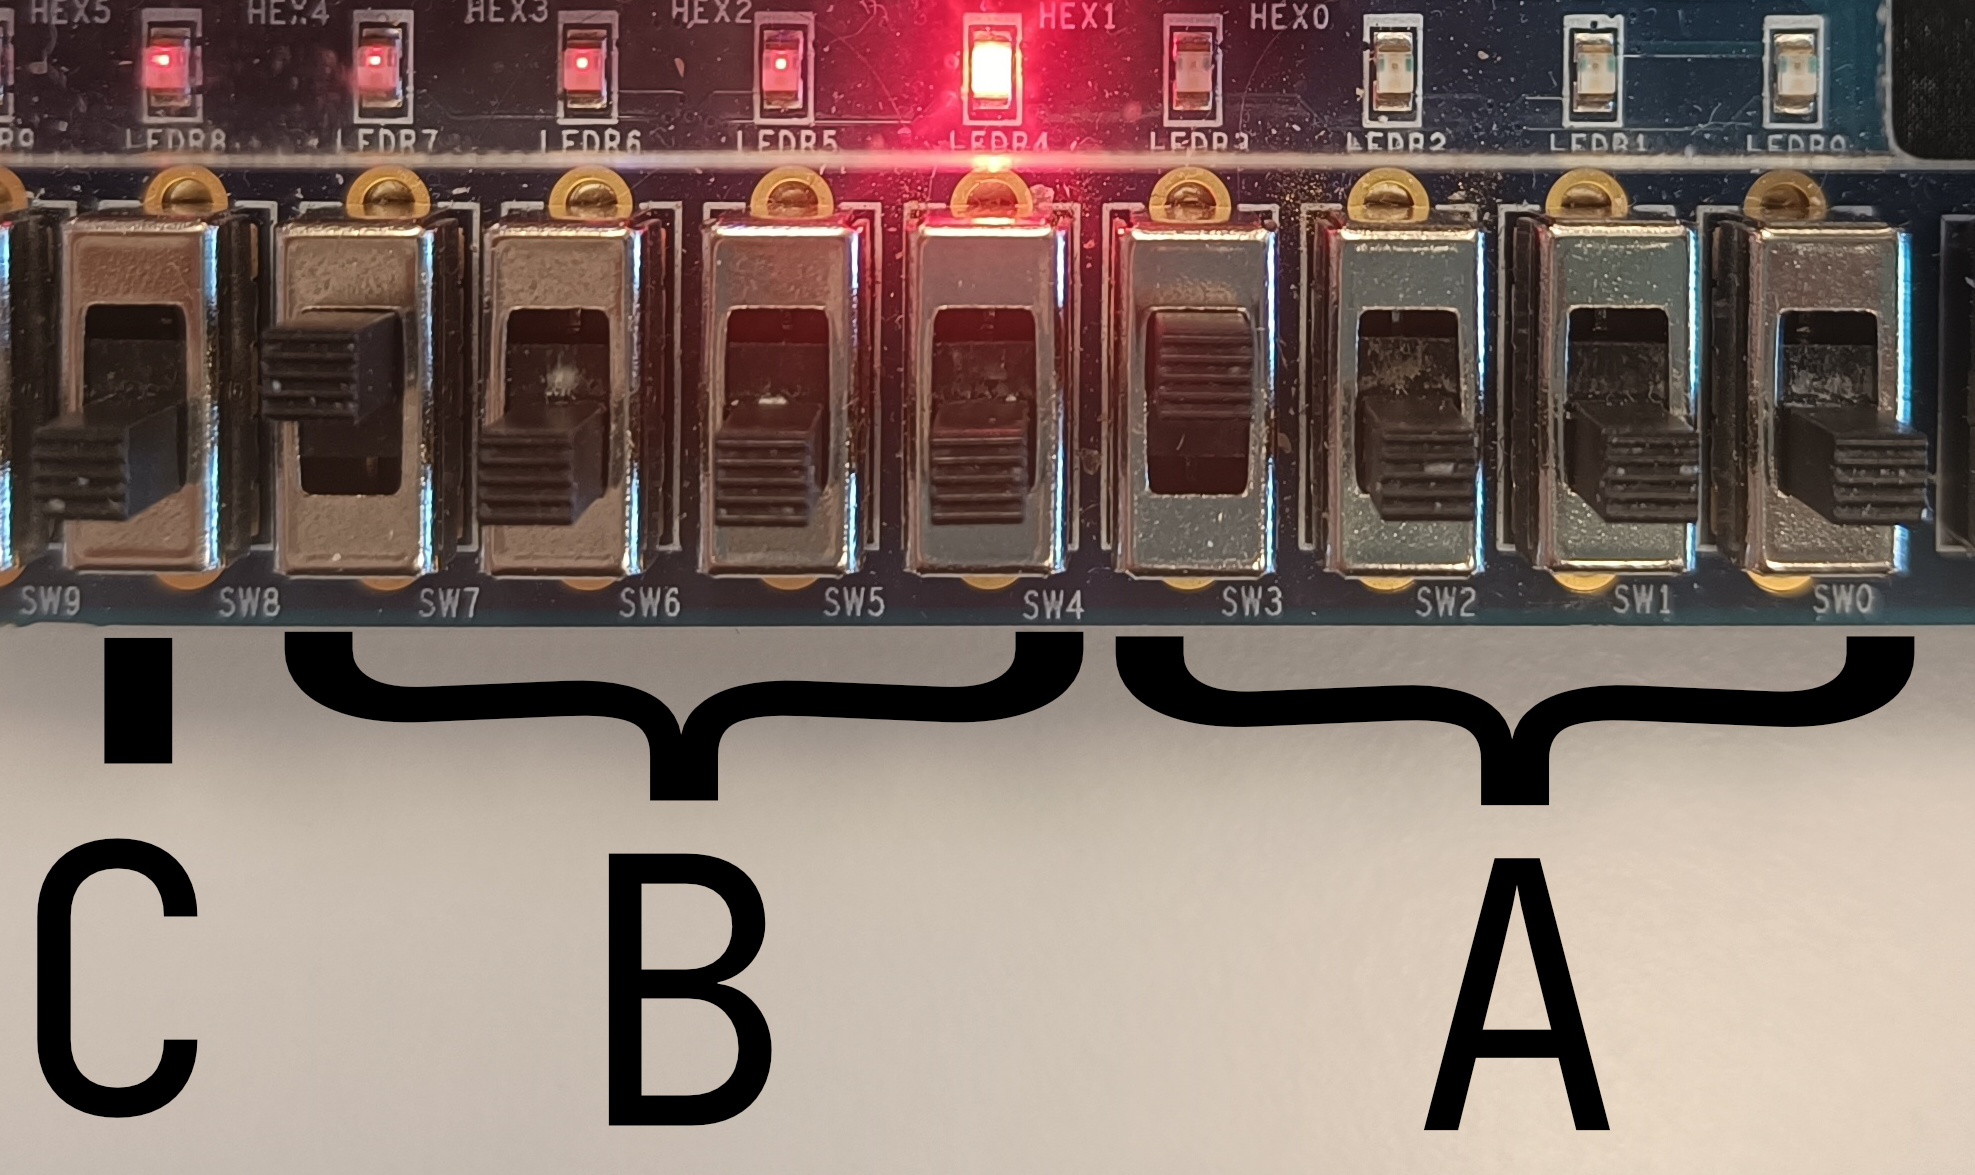
\includegraphics[width=1\textwidth]{Figures/Part3-0_8_8.jpg}
        \caption{0 + 8 + 8 = 16}
        \label{fig:T03pic3}
    \end{subfigure}
    \begin{subfigure}{0.4\textwidth}
        \centering
        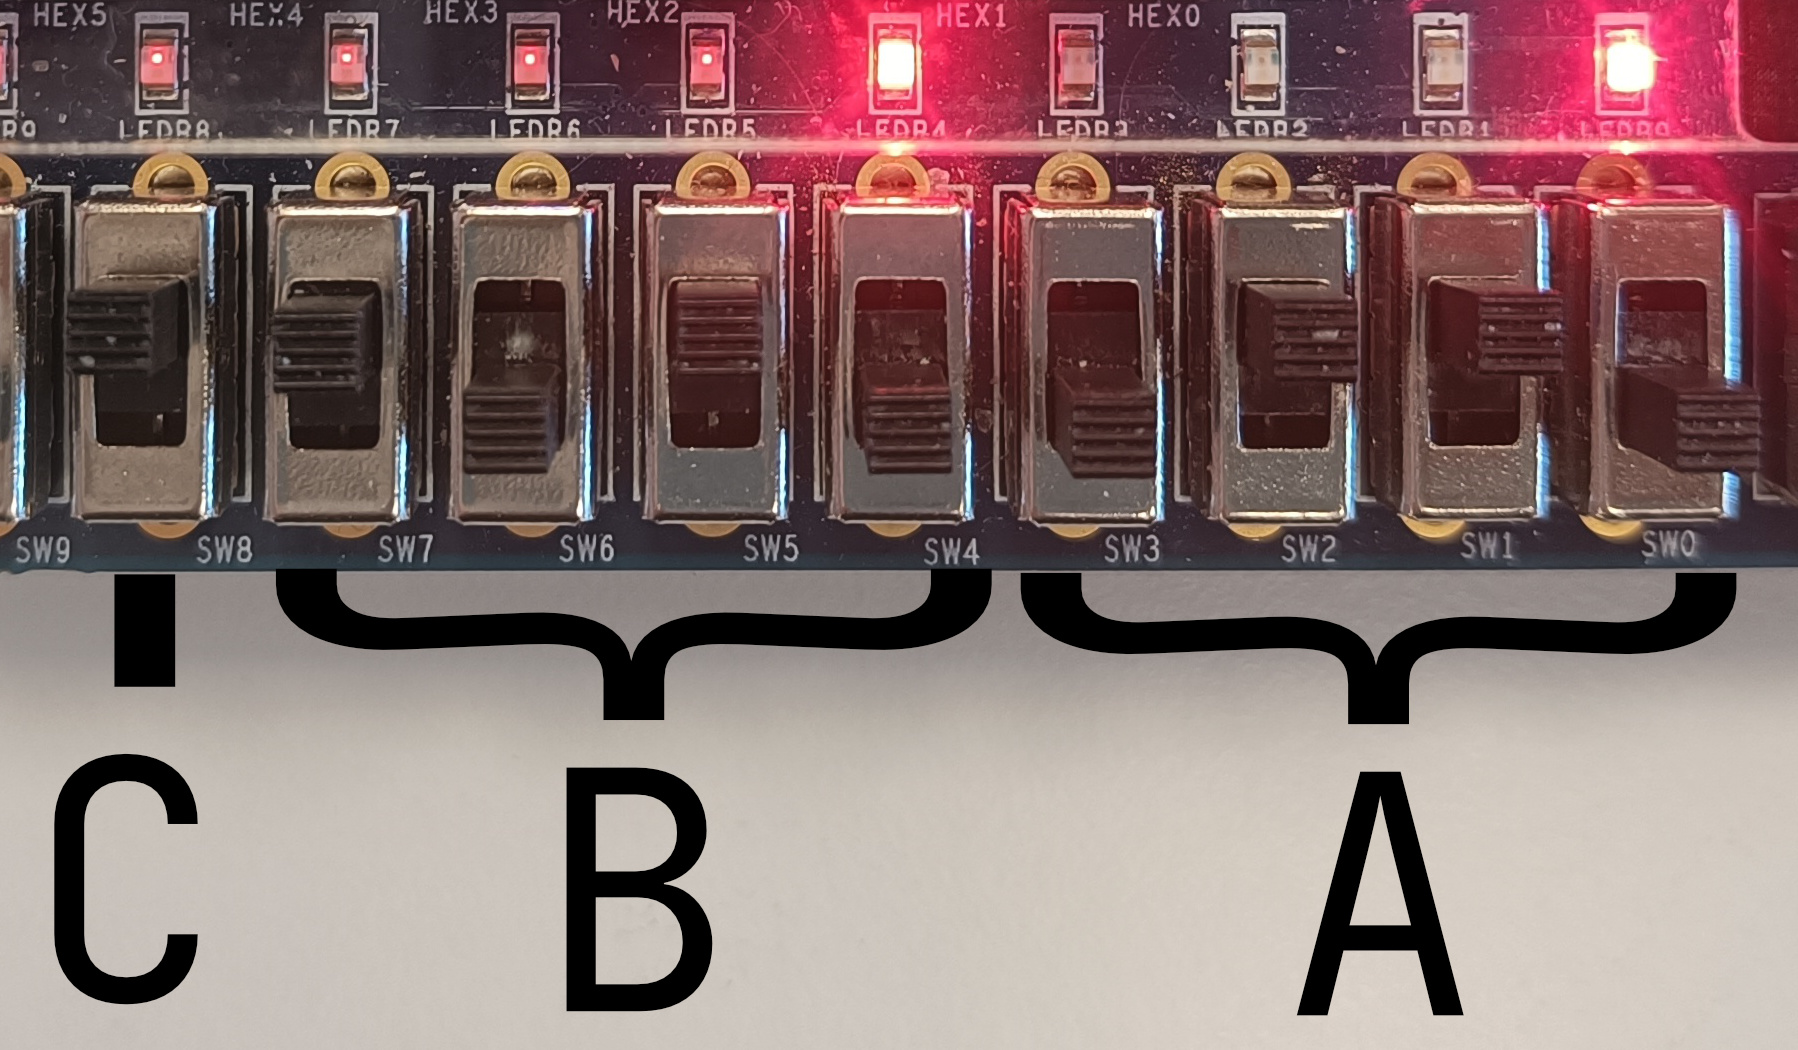
\includegraphics[width=1\textwidth]{Figures/Part3-1_10_6.jpg}
        \caption{1 + 10 + 6 = 17}
        \label{fig:T03pic4}
    \end{subfigure}
    \hfill
    \begin{subfigure}{0.4\textwidth}
        \centering
        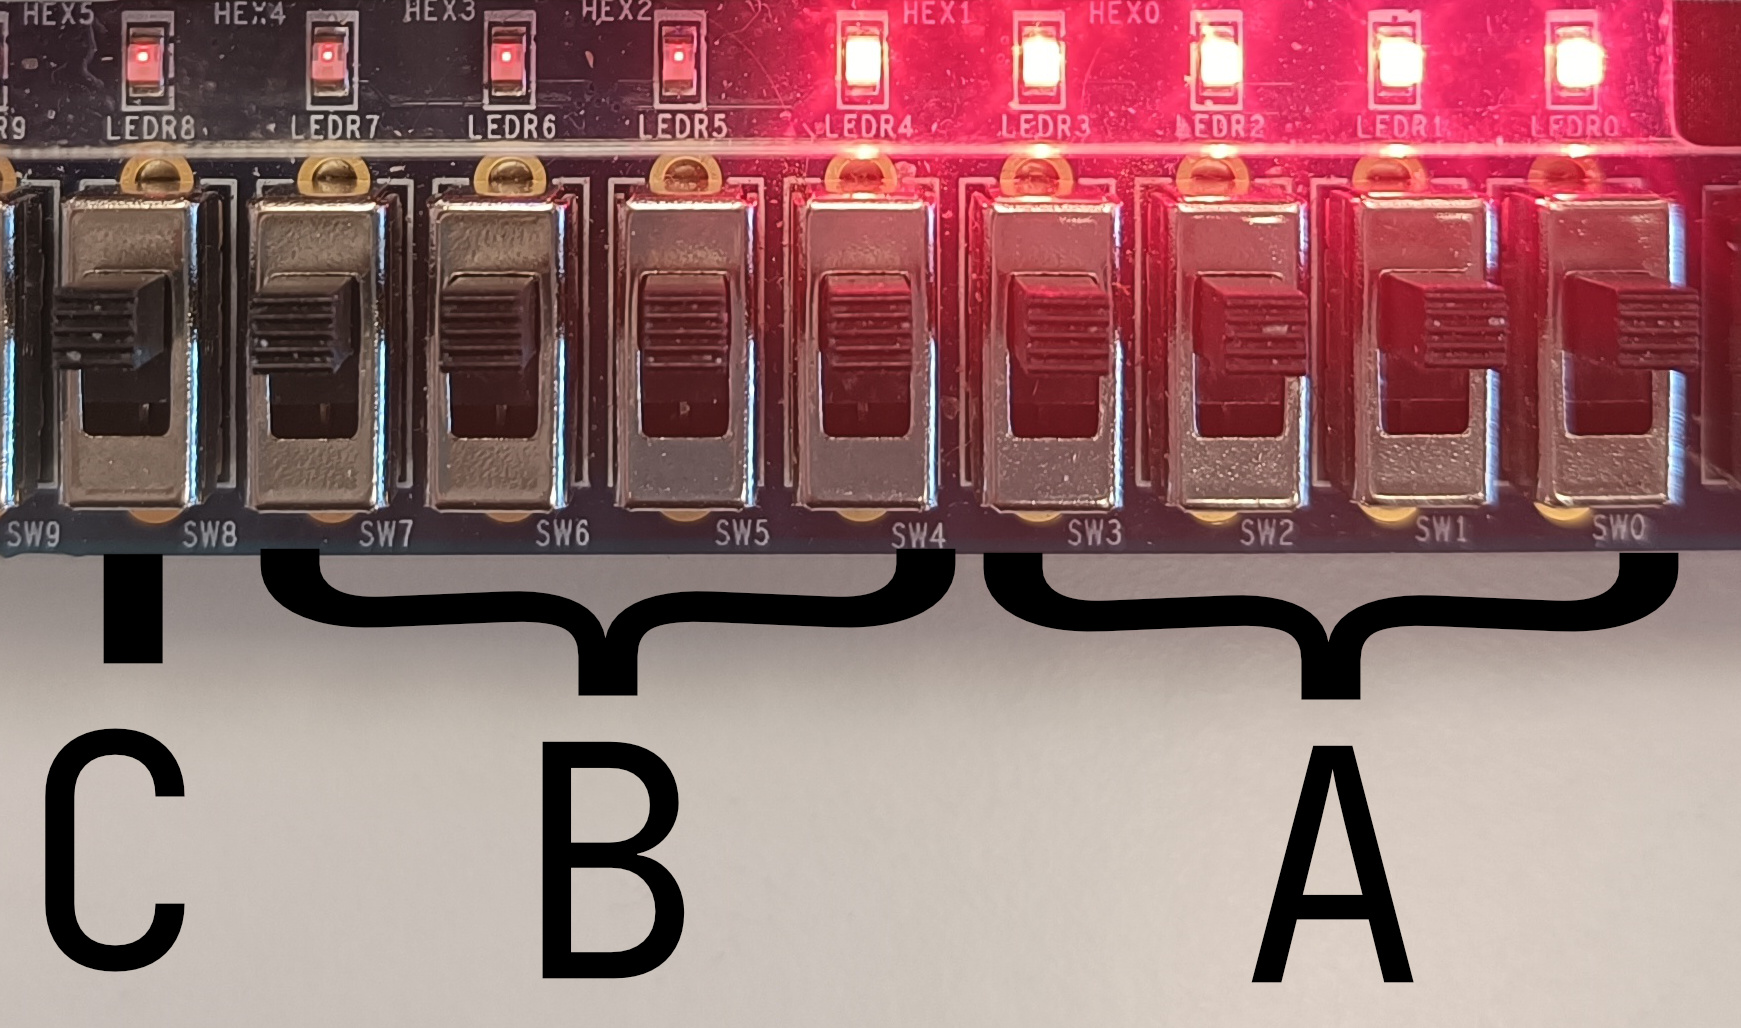
\includegraphics[width=1\textwidth]{Figures/Part3-1_15_15.jpg}
        \caption{1 + 15 + 15 = 31}
        \label{fig:T03pic5}
    \end{subfigure}
    \figcaption{Test results}
    \label{fig:T03pic}
\end{figure}


%   ############################## Section ##############################
\section{Part 4}
This part sort of combines part 2 and 3 with two 4 bit inputs and carry in and displays the result as a two digit decimal number. I used the same comparator method as in task 2, but extended for number up to 19 to check wether number is above 9. Then I modified the A circuit, renaming it T for transform to not mix up with the adder inputs and modifying it to convert 10-19 to 0-9.

\subsection{Code}

\writecode[VHDL]{Part4_TLE.vhd}{TLE as described in the task}
\clearpage
\writecode[VHDL]{Part4_4bitAdder.vhd}{4-bit adder used in TLE}
\clearpage
\writecode[VHDL]{Part4_adder.vhd}{Single bit adder used in 4-bit adder}
\writecode[VHDL]{Part4_mux.vhd}{Multiplexer used in TLE}
\clearpage
\writecode[VHDL]{Part4_decoder.vhd}{7-seg decoder used in TLE}

\clearpage
\subsection{RTL}
\begin{figure}[h]
    \centering
    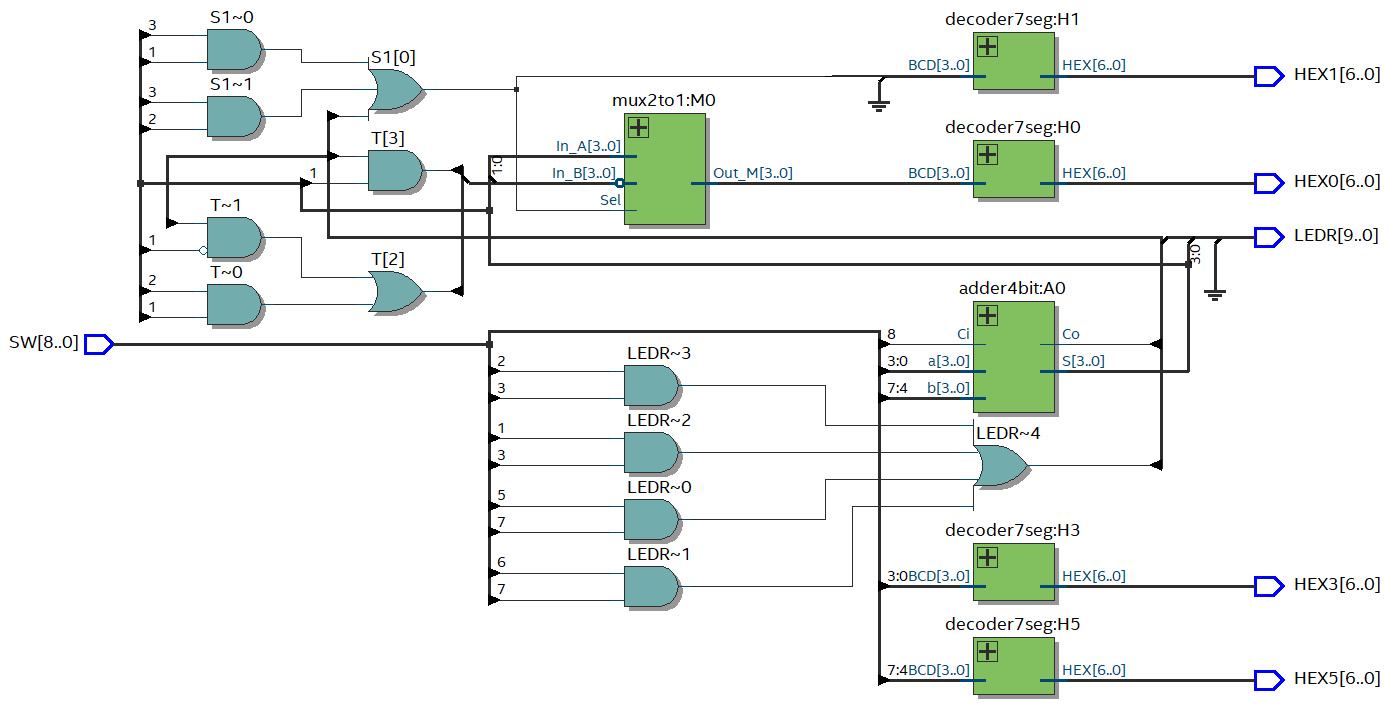
\includegraphics[width=1\textwidth]{Figures/Part4-RTL_TLE.jpg}
    \figcaption{RTL synthesizing of the TLE}
    \label{fig:T04rtl_tle}
\end{figure}
\begin{figure}[h]
    \centering
    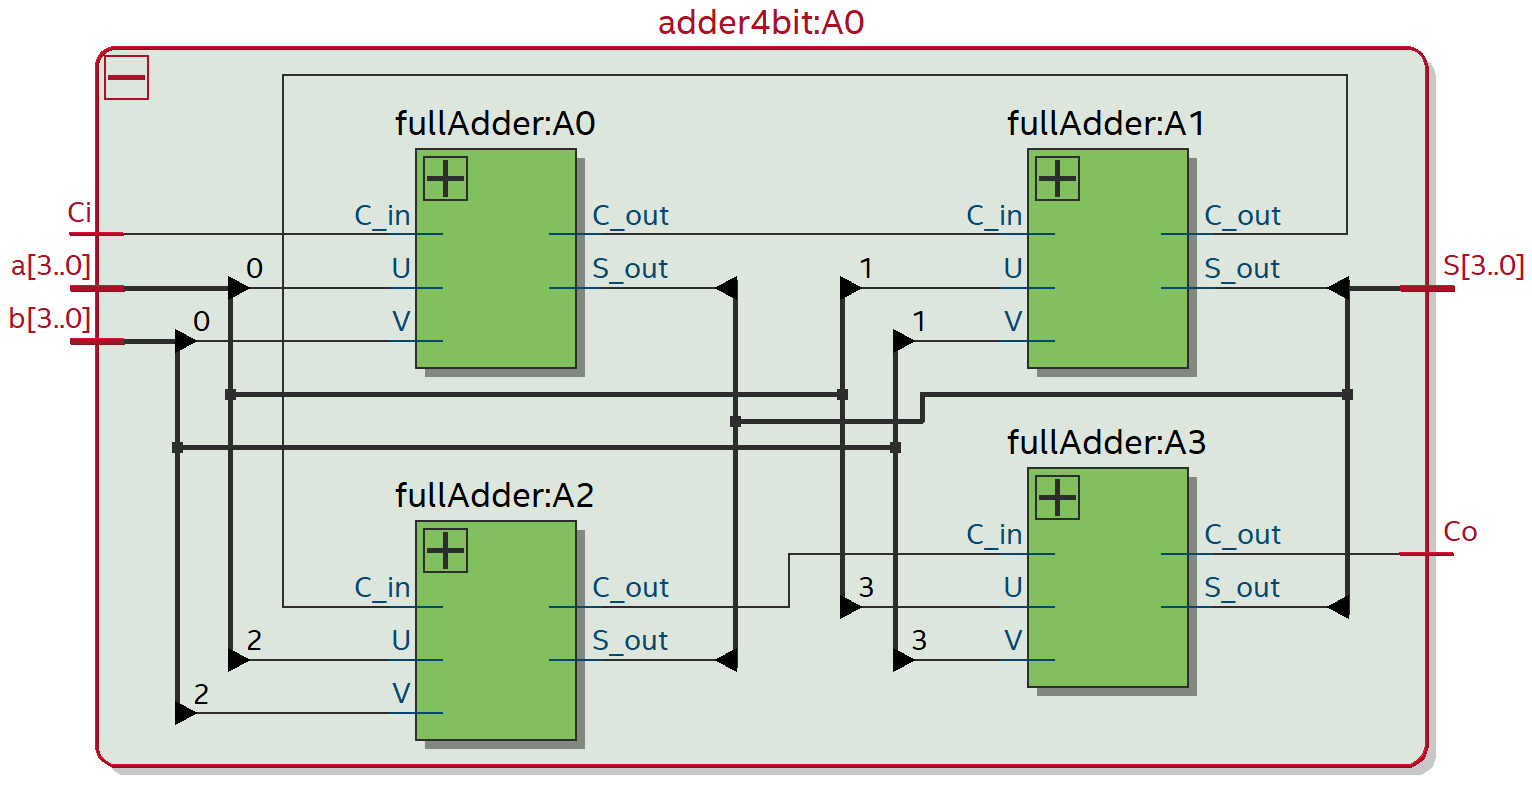
\includegraphics[width=1\textwidth]{Figures/Part4-RTL_adder4.jpg}
    \figcaption{RTL synthesizing of the 4 bit adder}
    \label{fig:T04rtl_adder4}
\end{figure}
\clearpage
\begin{figure}[h]
    \centering
    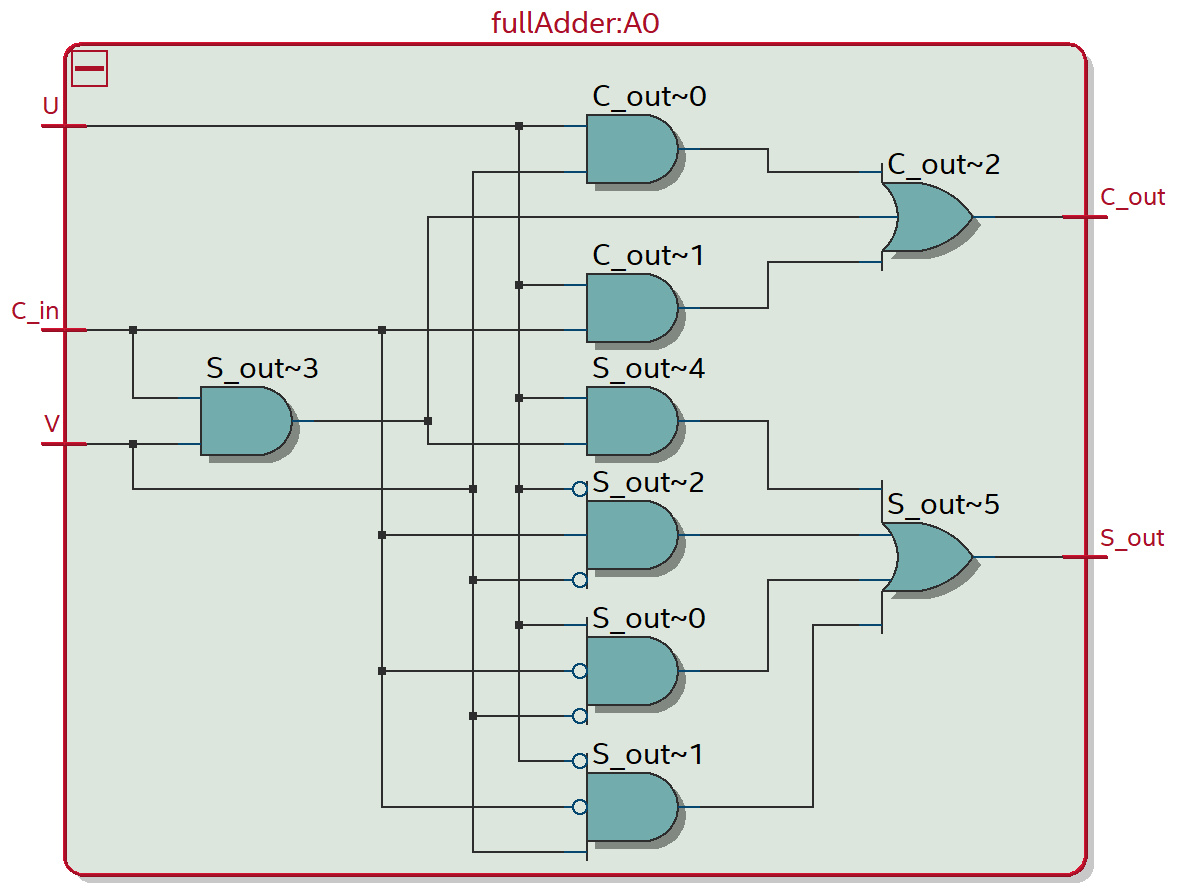
\includegraphics[width=1\textwidth]{Figures/Part4-RTL_adder1.jpg}
    \figcaption{RTL synthesizing of a single bit adder instance}
    \label{fig:T04rtl_adder1}
\end{figure}
\clearpage
\begin{figure}[h]
    \centering
    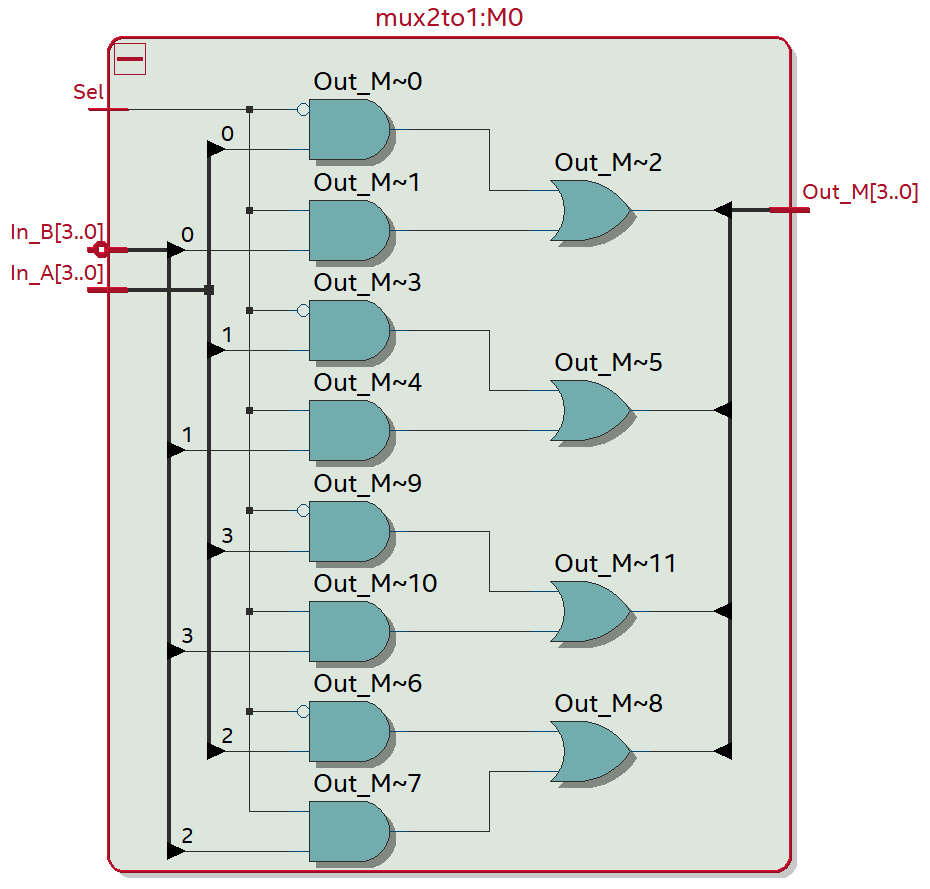
\includegraphics[width=1\textwidth]{Figures/Part4-RTL_mux.jpg}
    \figcaption{RTL synthesizing of the multiplexer}
    \label{fig:T04rtl_mux}
\end{figure}
\clearpage
\begin{figure}[h]
    \centering
    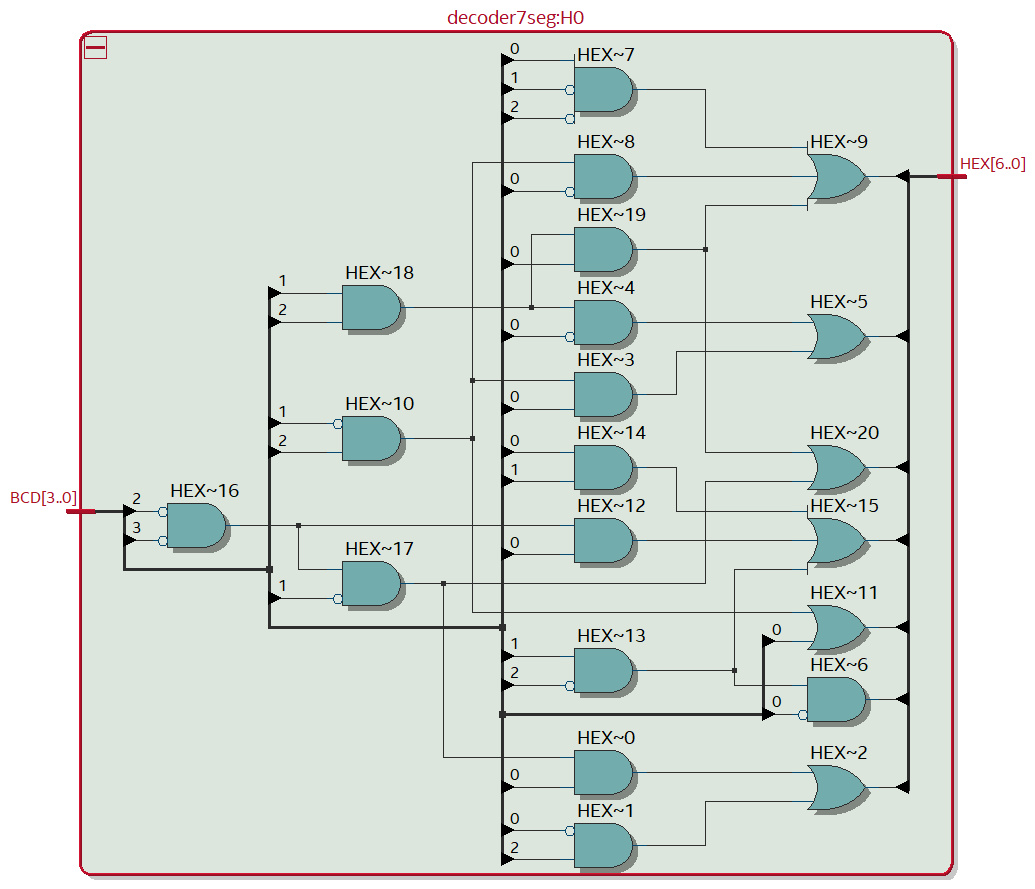
\includegraphics[width=1\textwidth]{Figures/Part4-RTL_decoder.jpg}
    \figcaption{RTL synthesizing of a 7-segment decoder instance}
    \label{fig:T04rtl_decoder}
\end{figure}

\clearpage
\subsection{Results}
\begin{figure}[h]
    \centering
    \begin{subfigure}{0.4\textwidth}
        \centering
        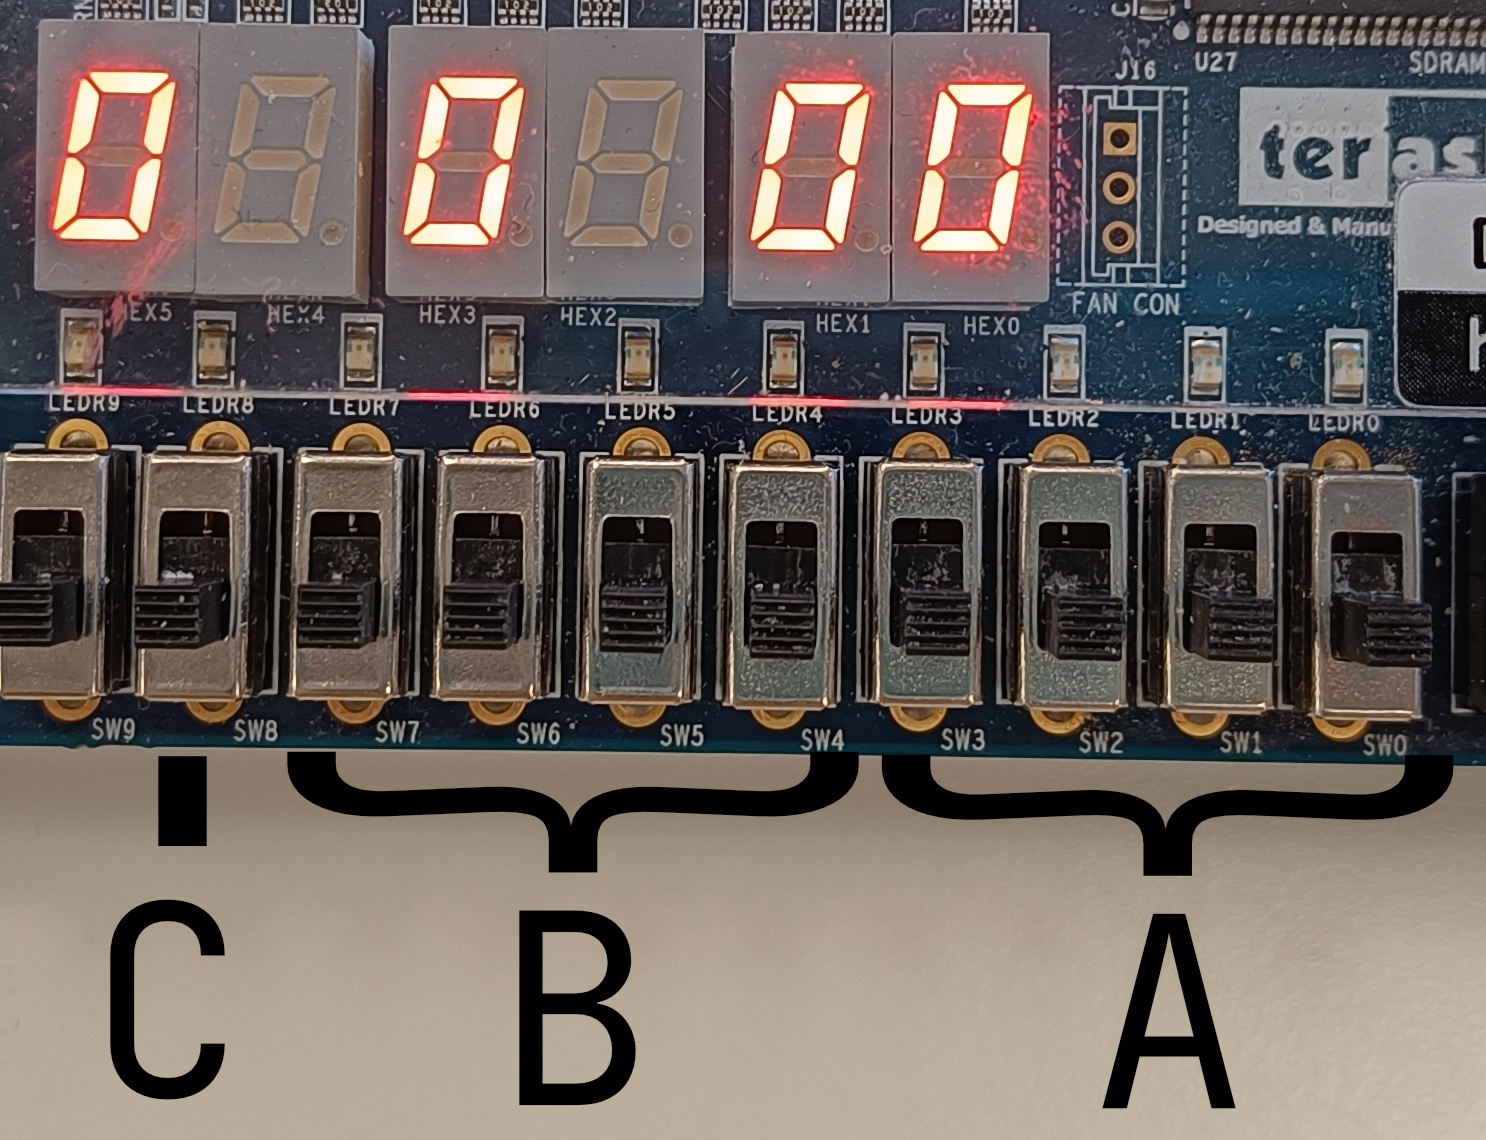
\includegraphics[width=1\textwidth]{Figures/Part4-0_0_0.jpg}
        \caption{0 + 0 + 0 = 0}
        \label{fig:T04pic1}
    \end{subfigure}
    \hfill
    \begin{subfigure}{0.4\textwidth}
        \centering
        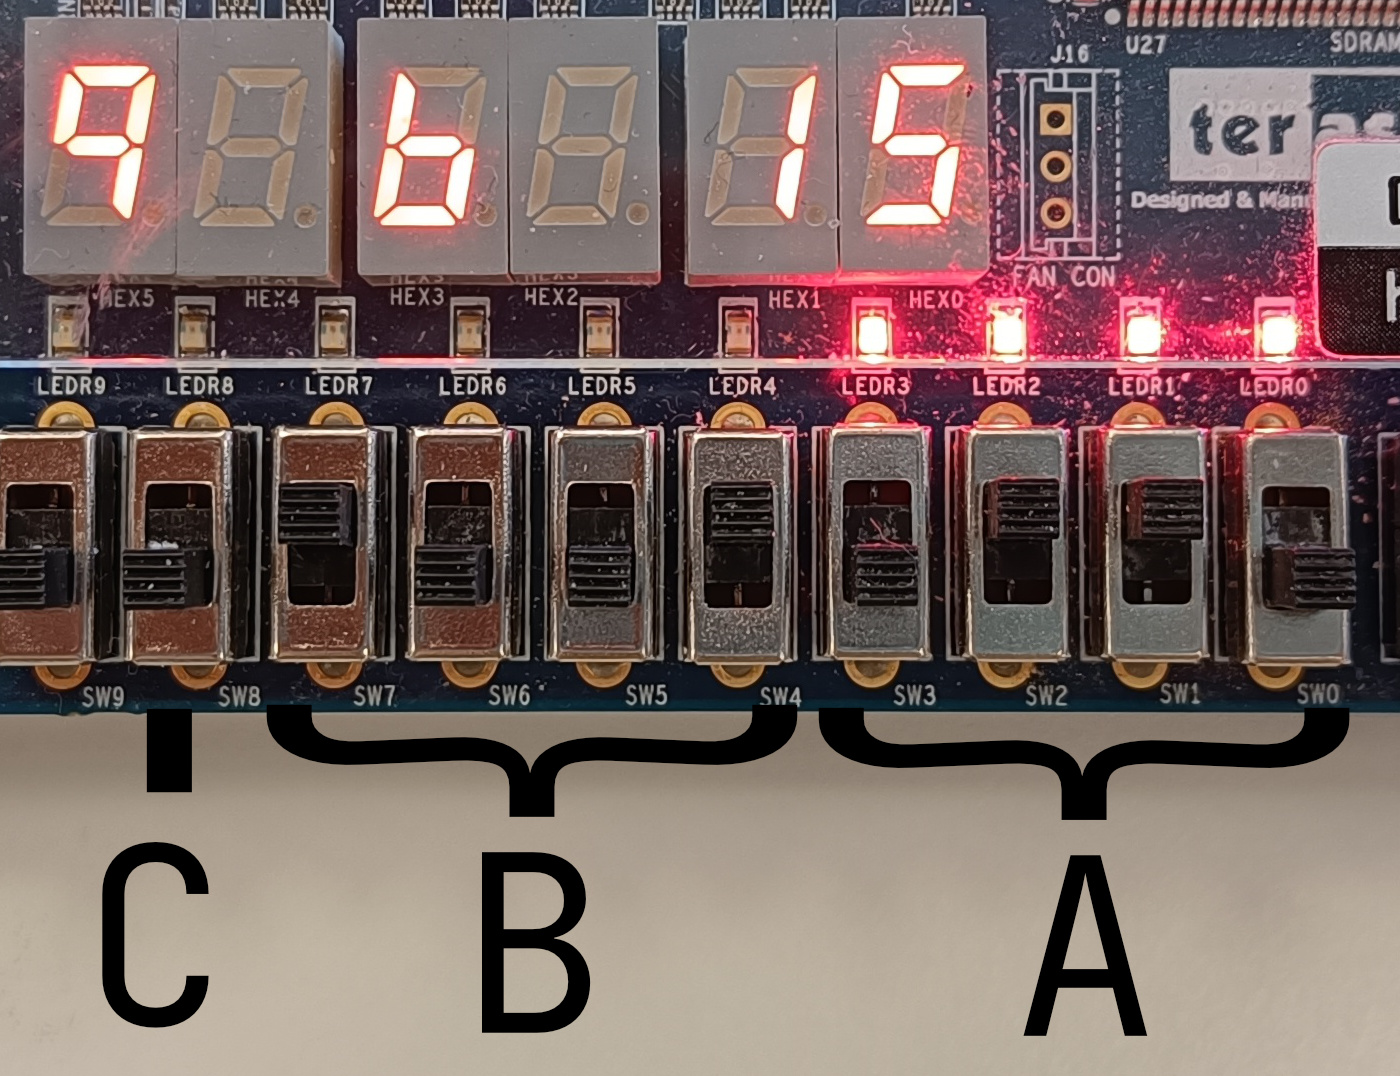
\includegraphics[width=1\textwidth]{Figures/Part4-0_9_6.jpg}
        \caption{0 + 9 + 6 = 15}
        \label{fig:T04pic2}
    \end{subfigure}
    \begin{subfigure}{0.4\textwidth}
        \centering
        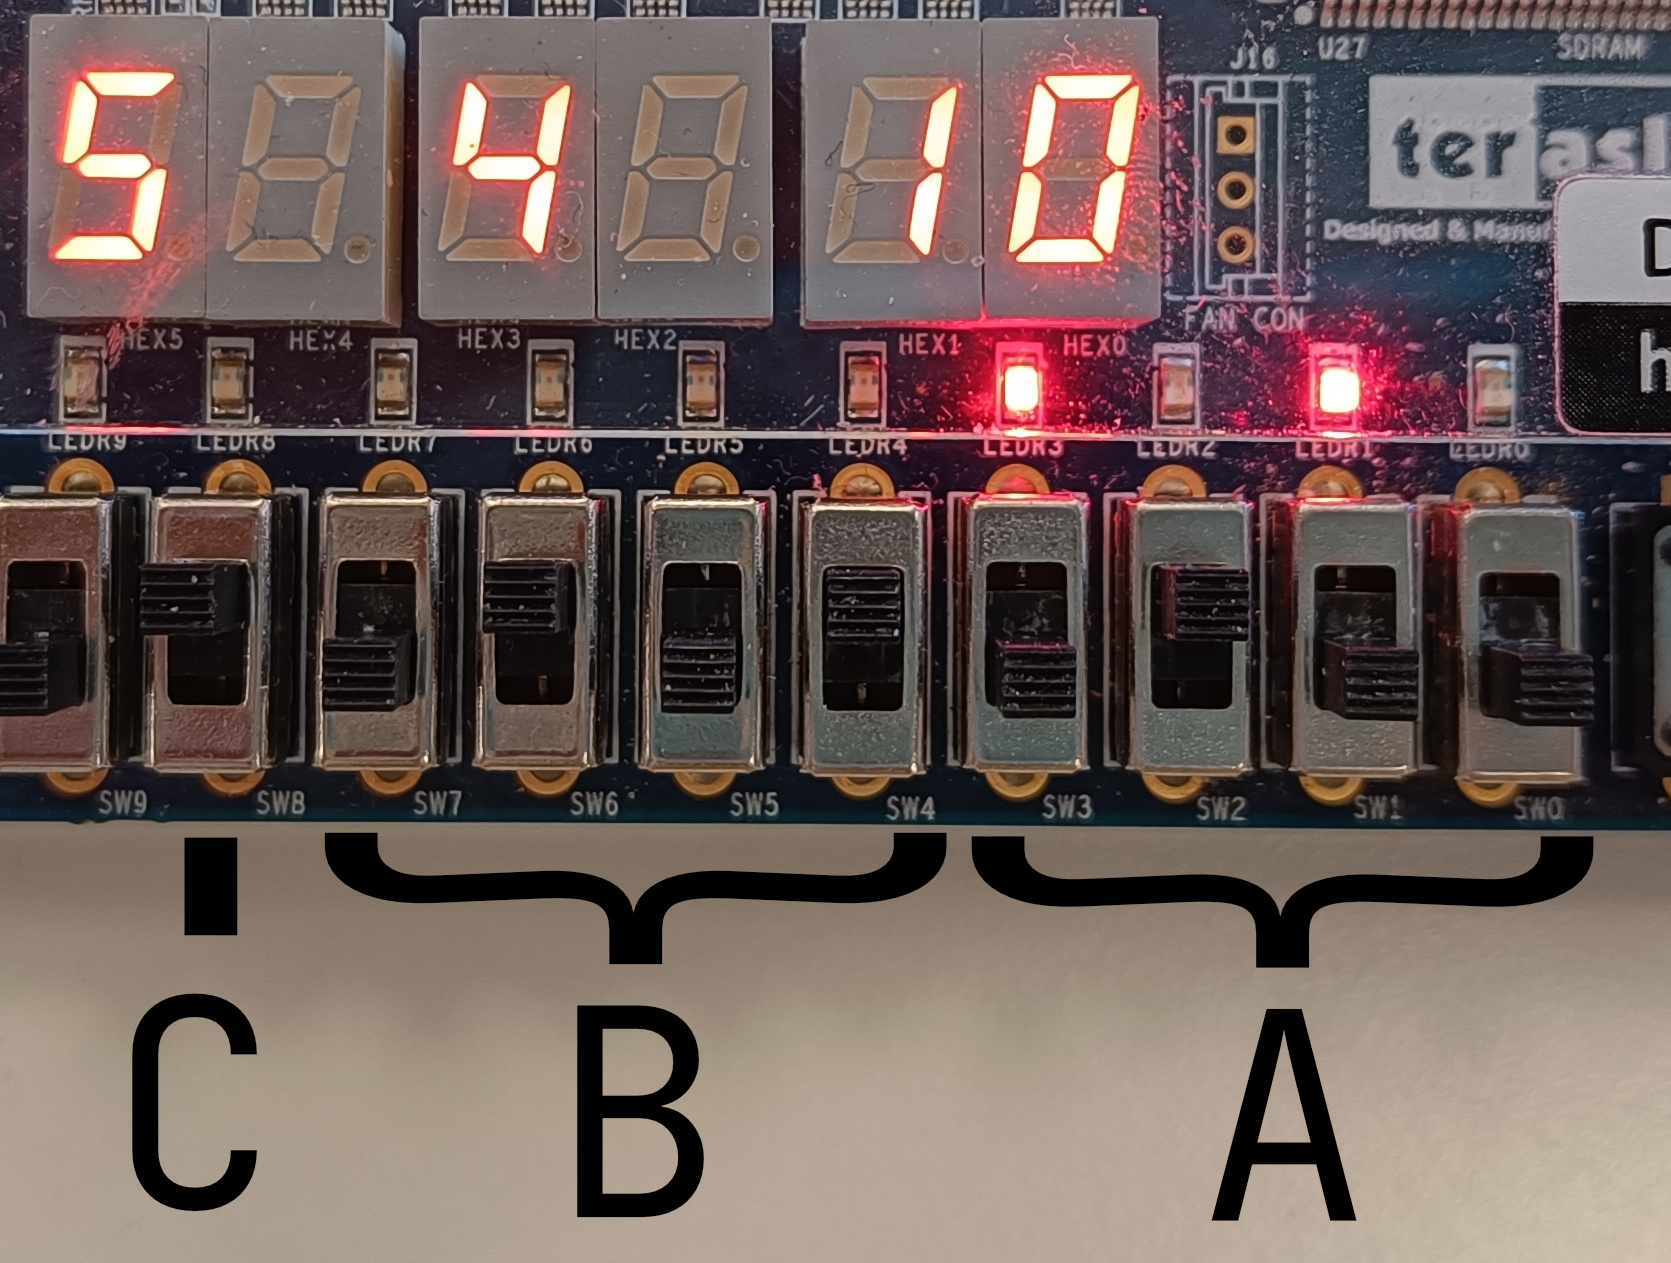
\includegraphics[width=1\textwidth]{Figures/Part4-1_5_4.jpg}
        \caption{1 + 5 + 4 = 10}
        \label{fig:T04pic3}
    \end{subfigure}
    \hfill
    \begin{subfigure}{0.4\textwidth}
        \centering
        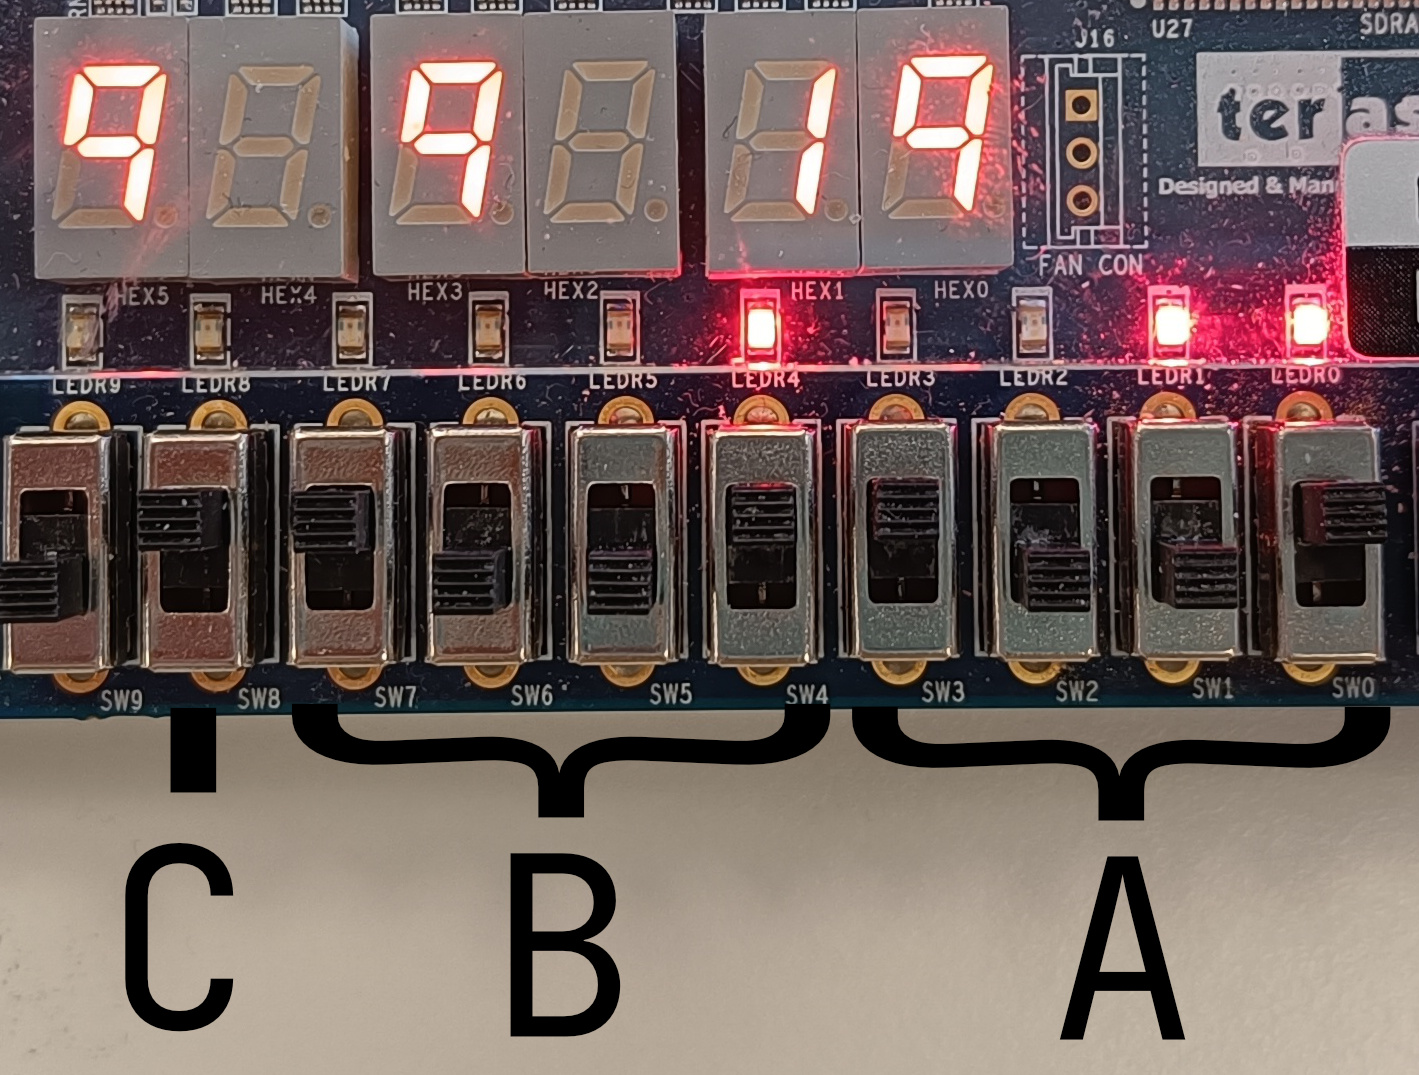
\includegraphics[width=1\textwidth]{Figures/Part4-1_9_9.jpg}
        \caption{1 + 9 + 9 = 19}
        \label{fig:T04pic4}
    \end{subfigure}
    \begin{subfigure}{0.4\textwidth}
        \centering
        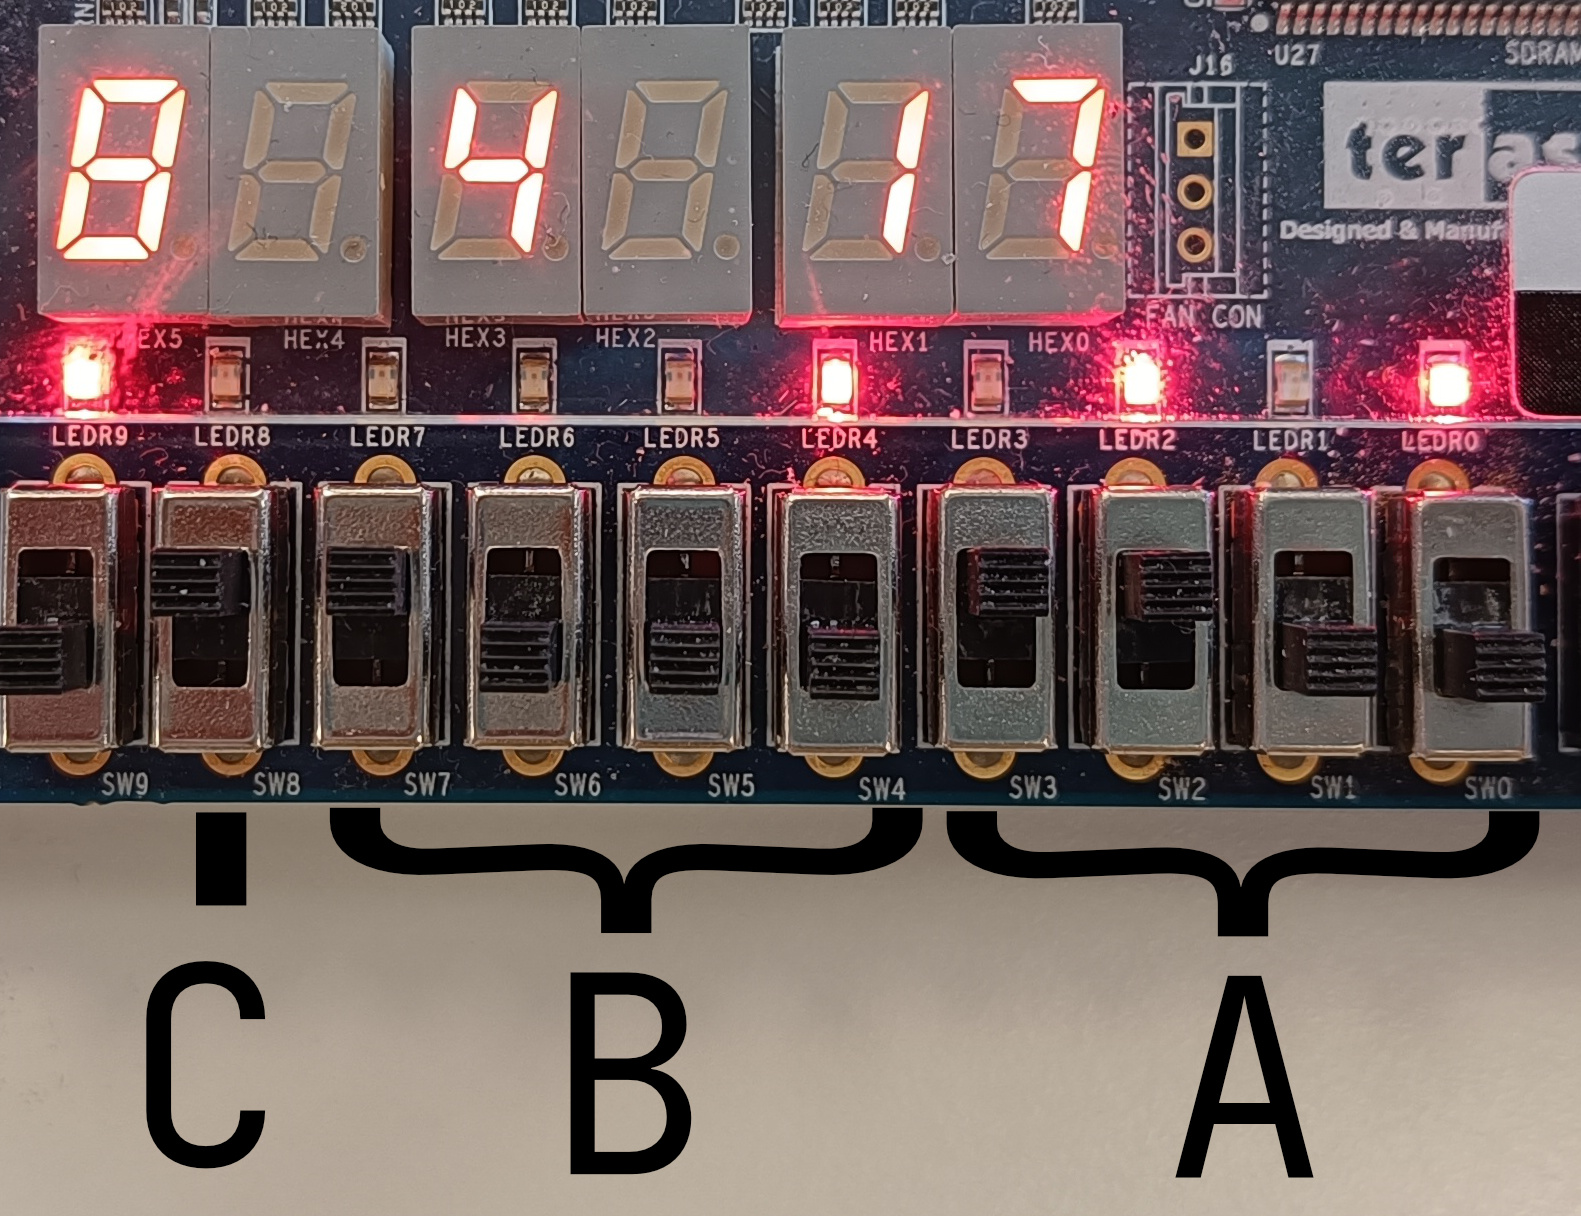
\includegraphics[width=1\textwidth]{Figures/Part4-1_8_12.jpg}
        \caption{Out of bounds}
        \label{fig:T04pic5}
    \end{subfigure}
    \hfill
    \begin{subfigure}{0.4\textwidth}
        \centering
        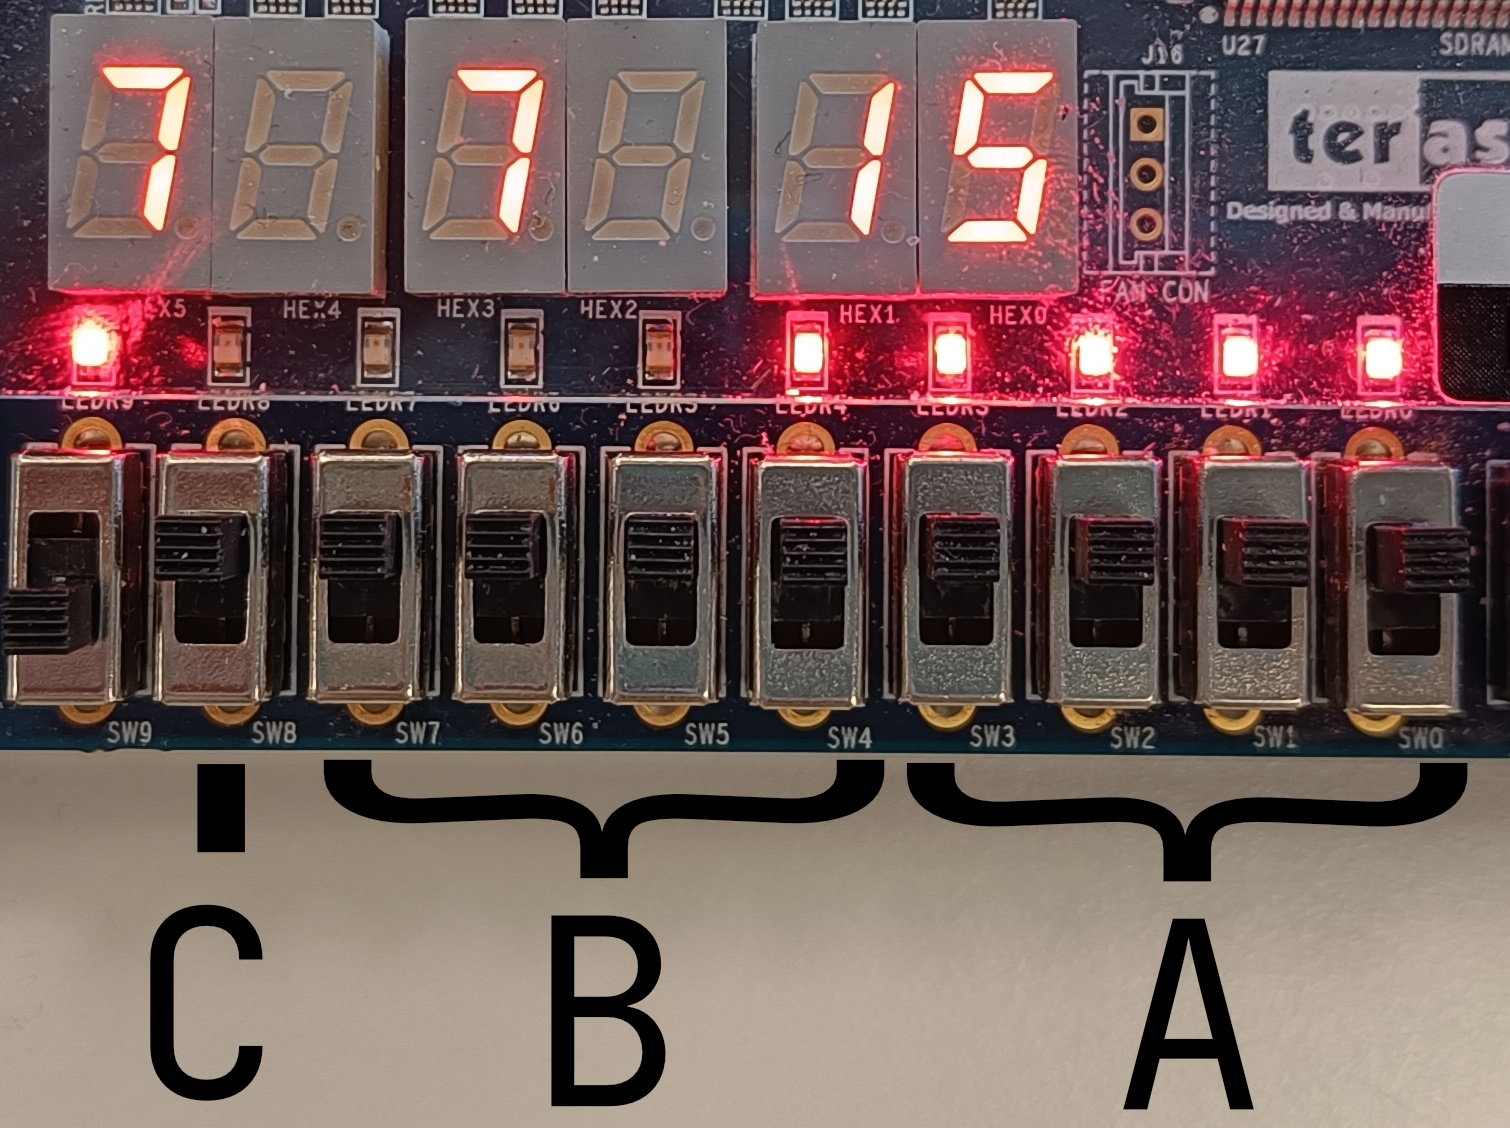
\includegraphics[width=1\textwidth]{Figures/Part4-1_15_15.jpg}
        \caption{Out of bounds}
        \label{fig:T04pic6}
    \end{subfigure}
    \figcaption{Test results}
    \label{fig:T04pic}
\end{figure}


%   ############################## Section ##############################
\section{Part 5}

\subsection{Code}

\writecode[VHDL]{Part5_TLE.vhd}{TLE as described in the task}
\writecode[VHDL]{Part5_decoder.vhd}{7-seg decoder used in TLE}

\clearpage
\subsection{RTL}
\begin{figure}[h]
    \centering
    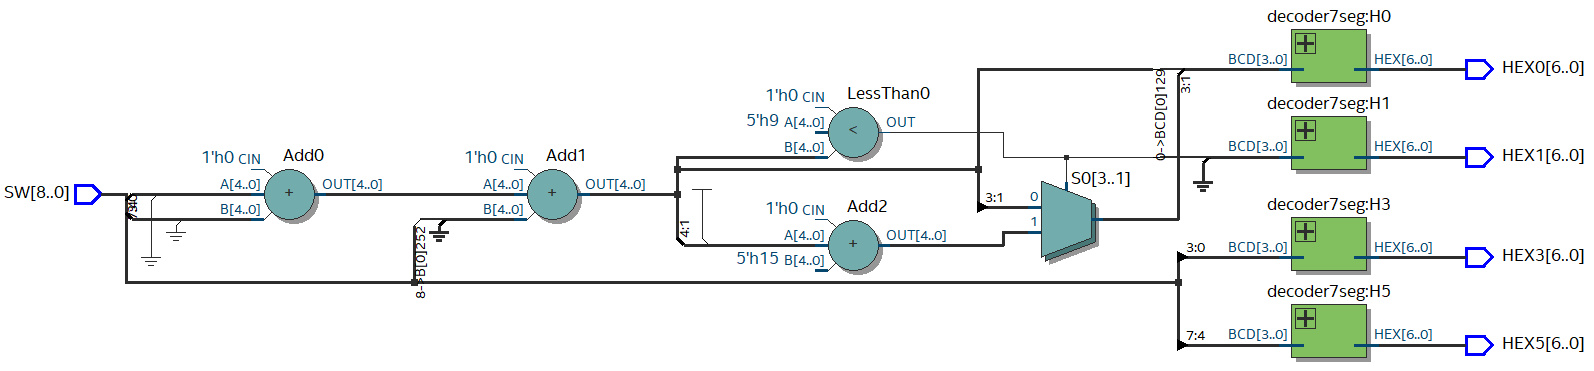
\includegraphics[width=1\textwidth]{Figures/Part5-RTL_TLE.jpg}
    \figcaption{RTL synthesizing of the TLE}
    \label{fig:T05rtl_tle}
\end{figure}
\begin{figure}[h]
    \centering
    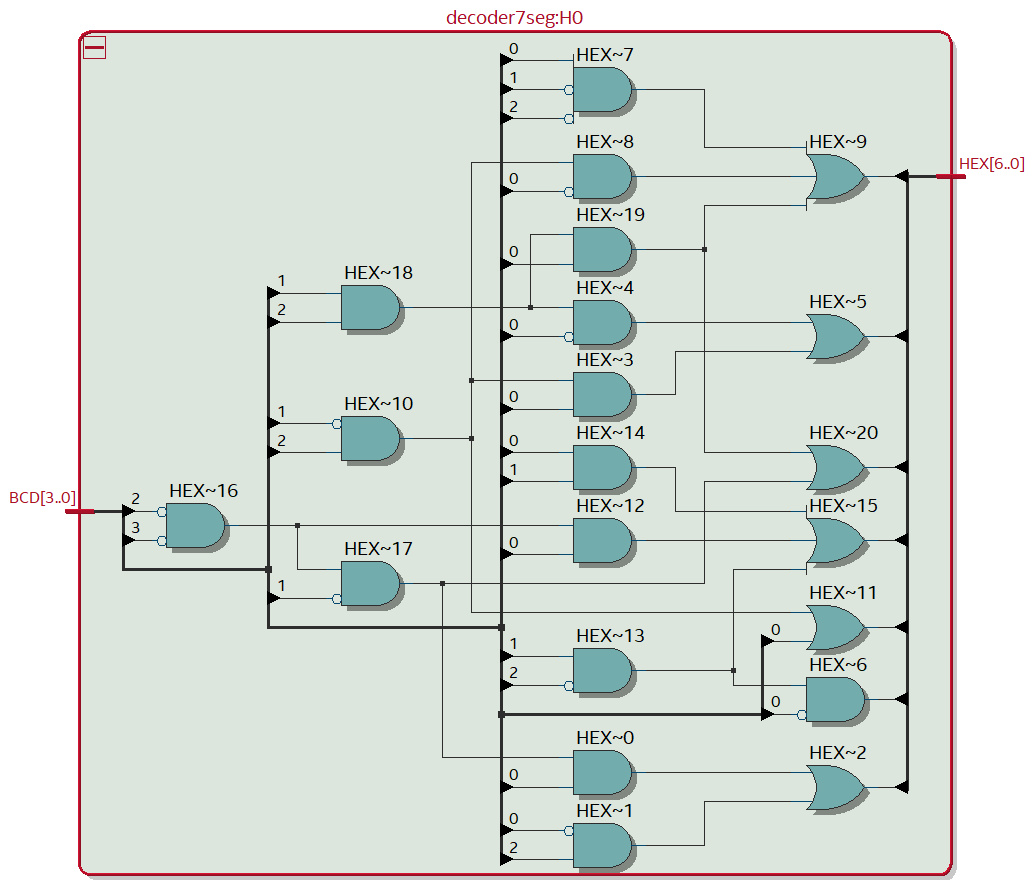
\includegraphics[width=0.95\textwidth]{Figures/Part5-RTL_decoder.jpg}
    \figcaption{RTL synthesizing of the 7-segment decoder}
    \label{fig:T04rtl_decoder}
\end{figure}

\clearpage
\subsection{Results}
\begin{figure}[h]
    \centering
    \begin{subfigure}{0.4\textwidth}
        \centering
        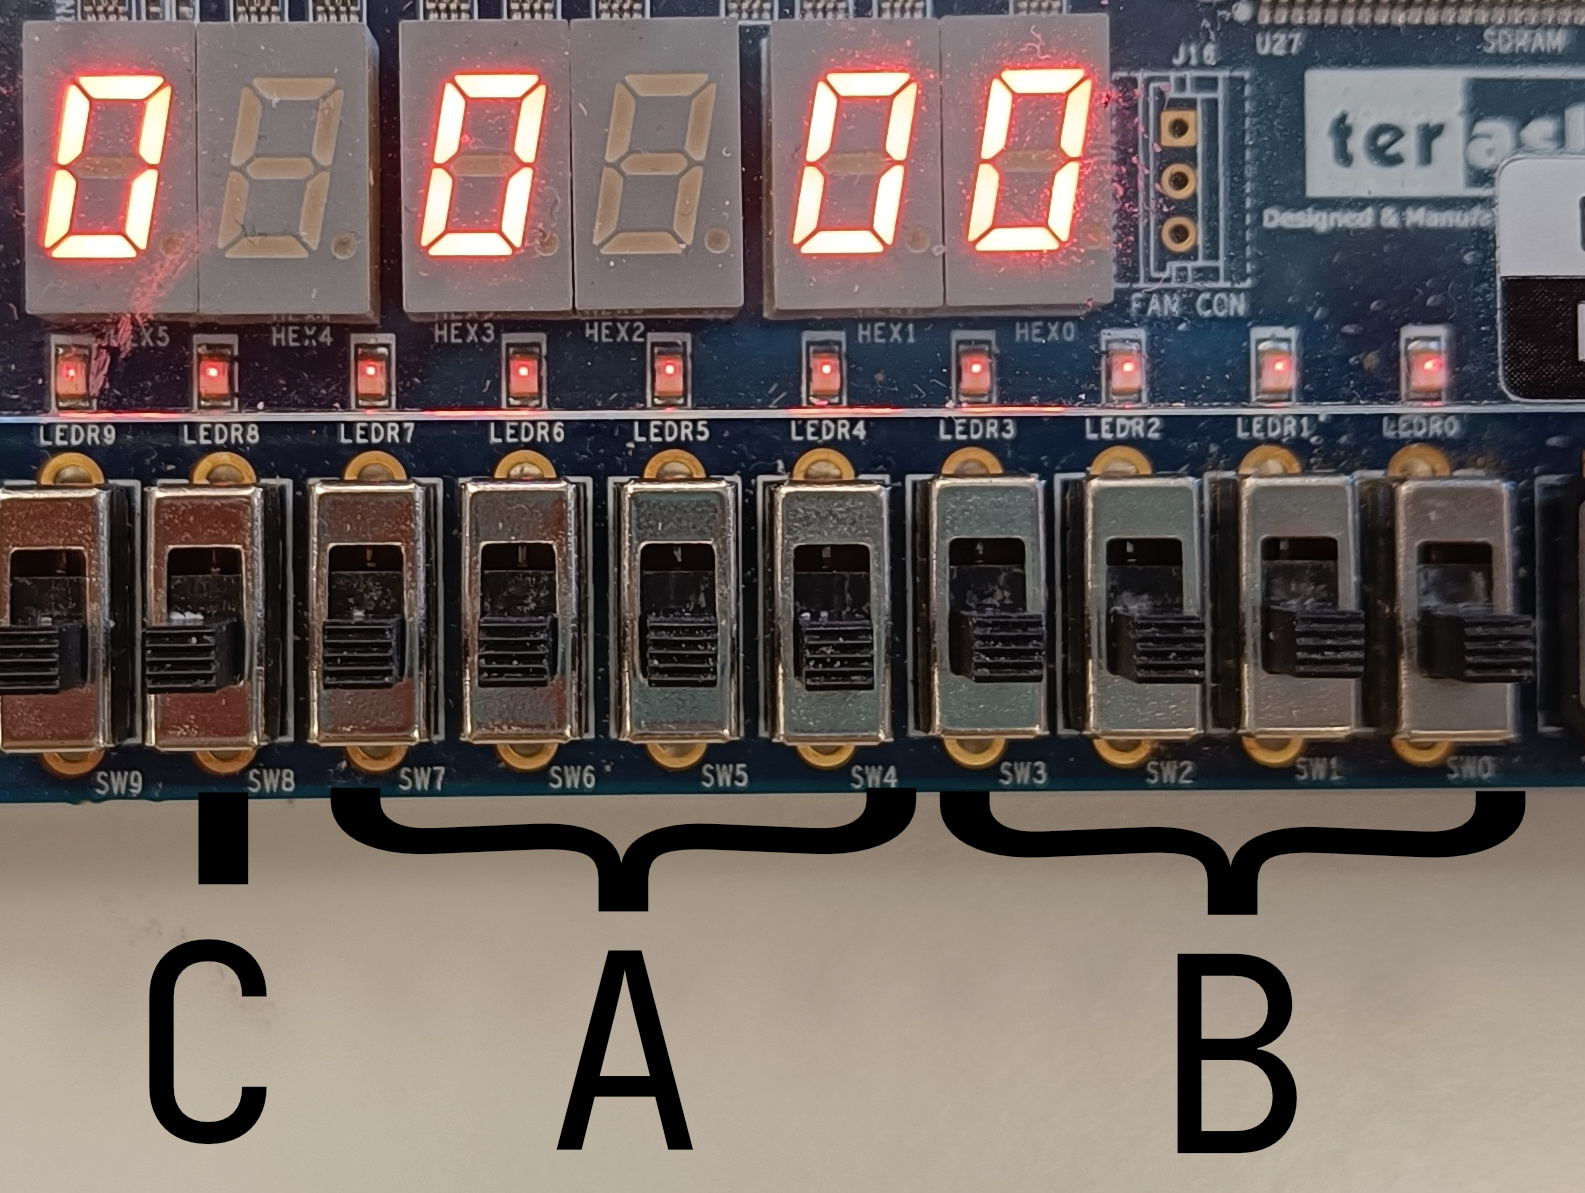
\includegraphics[width=1\textwidth]{Figures/Part5-0_0_0.jpg}
        \caption{0 + 0 + 0 = 0}
        \label{fig:T05pic1}
    \end{subfigure}
    \hfill
    \begin{subfigure}{0.4\textwidth}
        \centering
        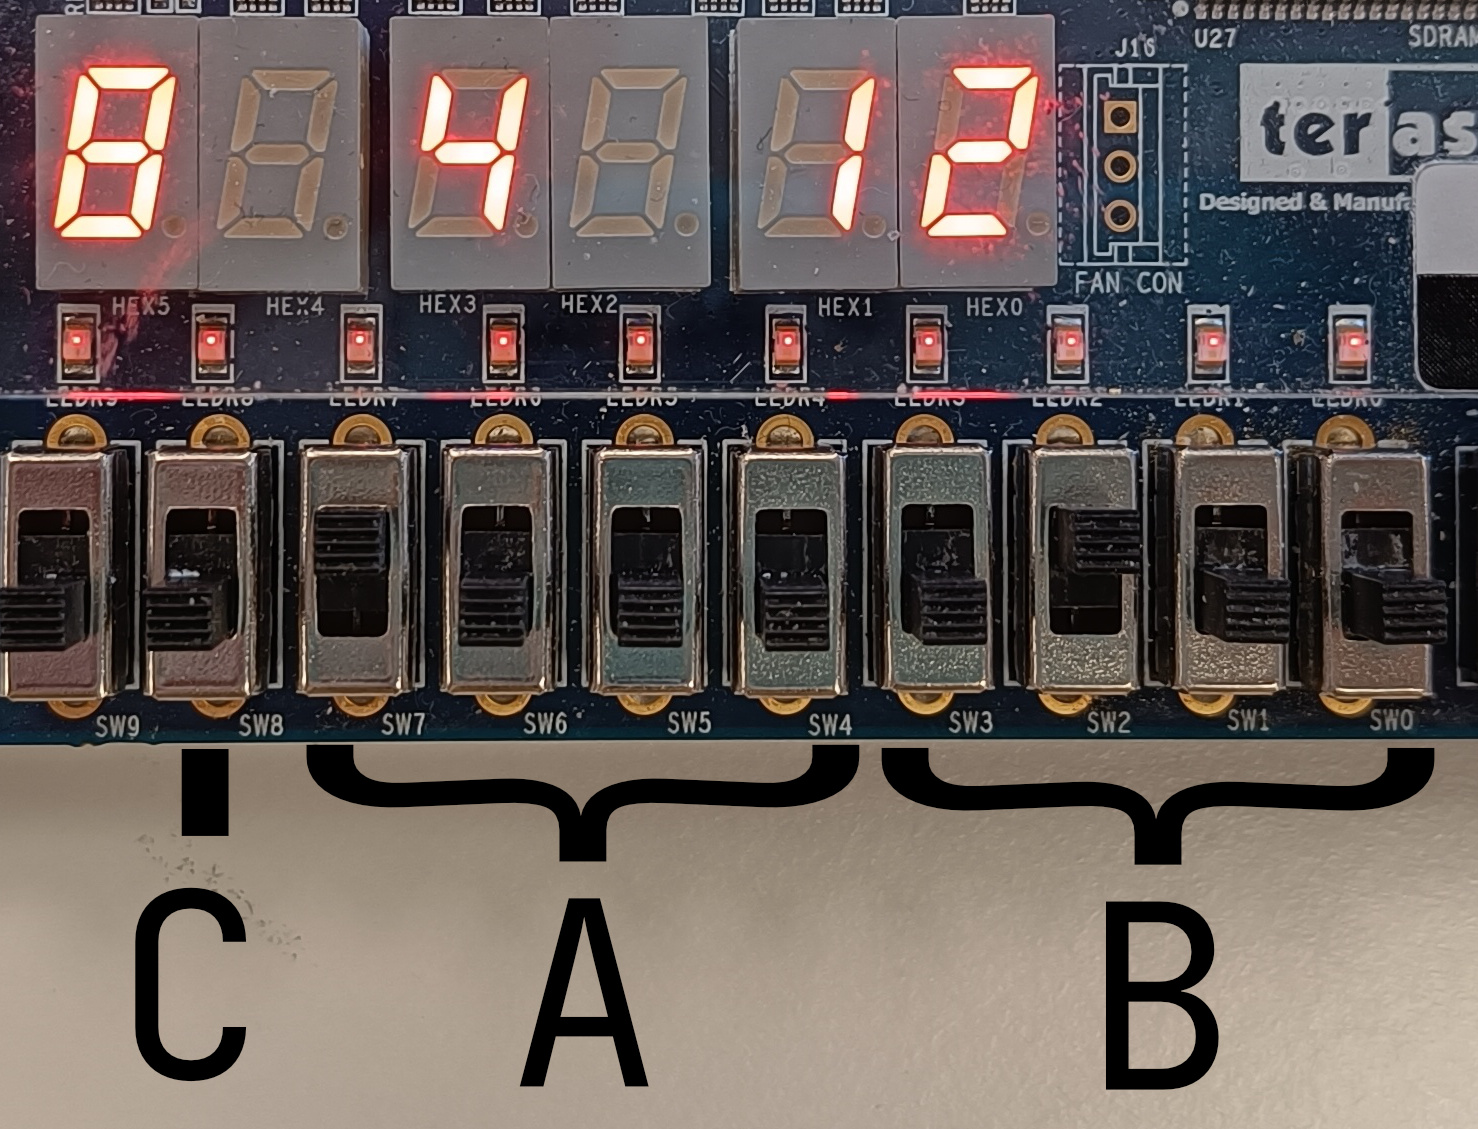
\includegraphics[width=1\textwidth]{Figures/Part5-0_8_4.jpg}
        \caption{0 + 8 + 4 = 12}
        \label{fig:T05pic2}
    \end{subfigure}
    \begin{subfigure}{0.4\textwidth}
        \centering
        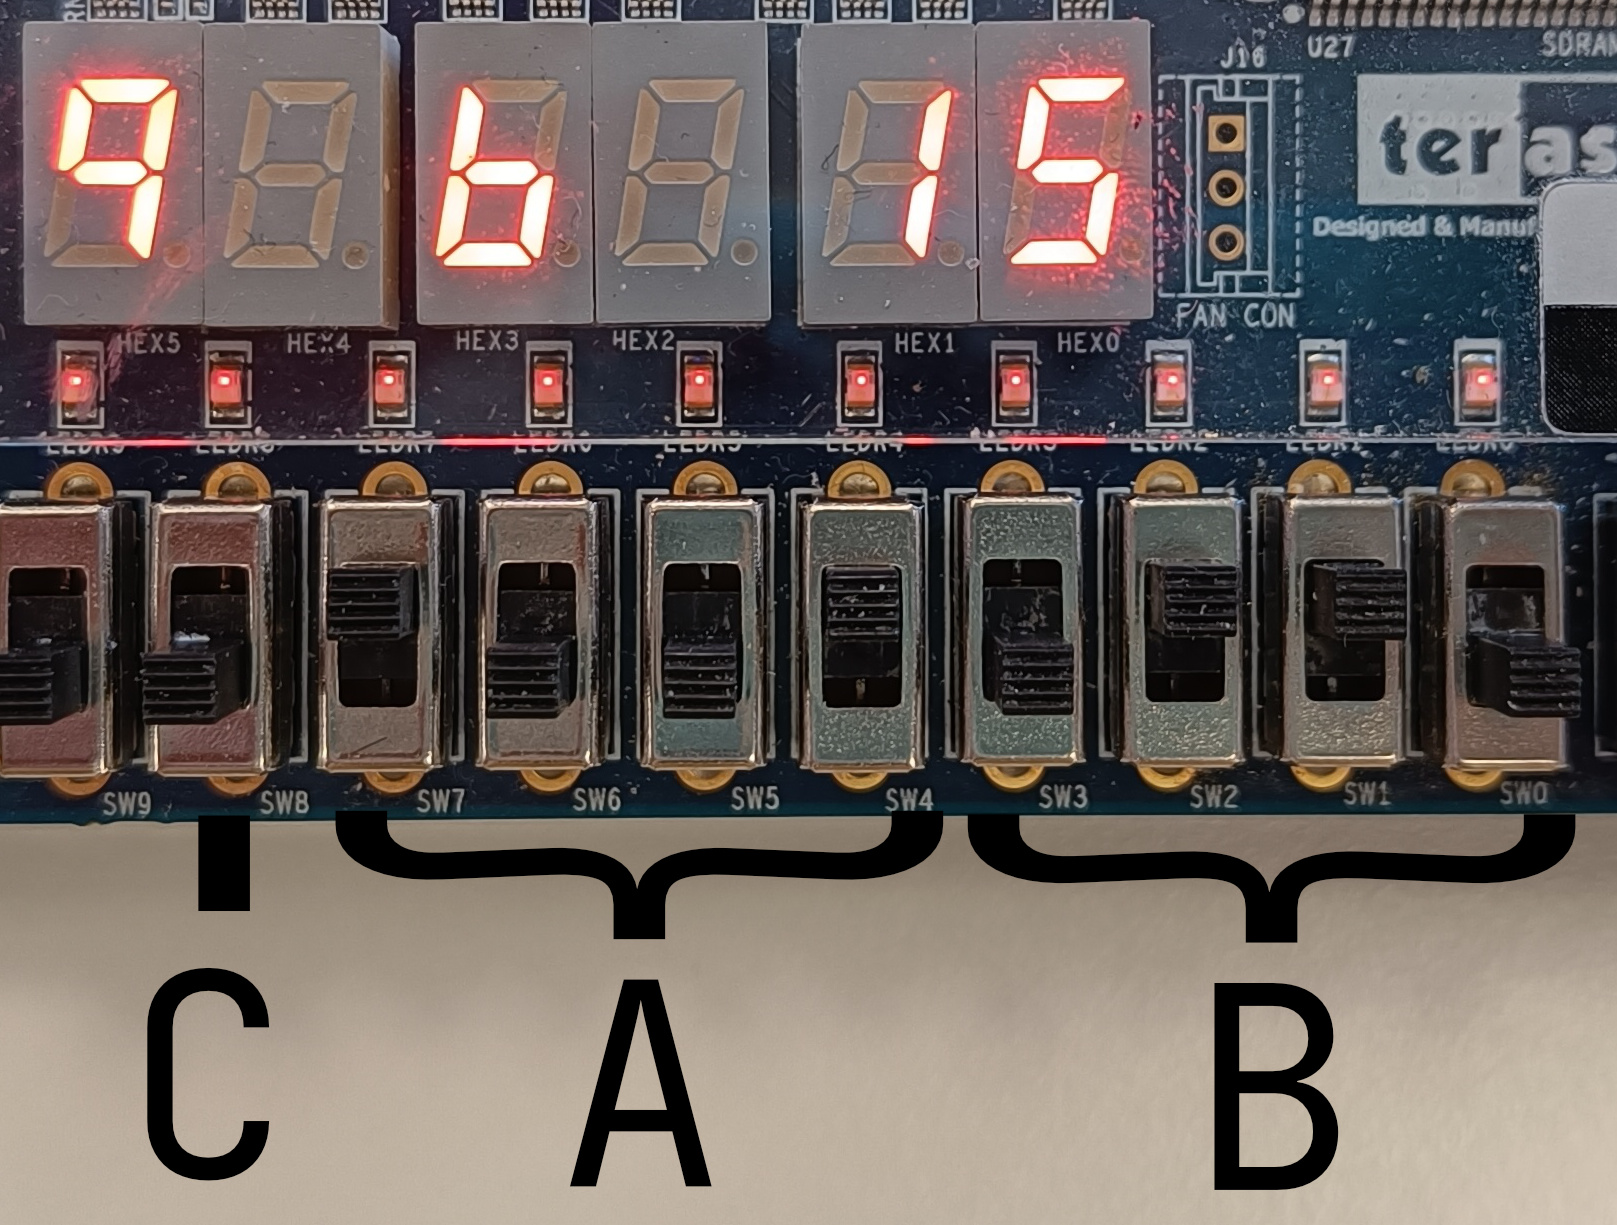
\includegraphics[width=1\textwidth]{Figures/Part5-0_9_6.jpg}
        \caption{0 + 9 + 6 = 15}
        \label{fig:T05pic3}
    \end{subfigure}
    \hfill
    \begin{subfigure}{0.4\textwidth}
        \centering
        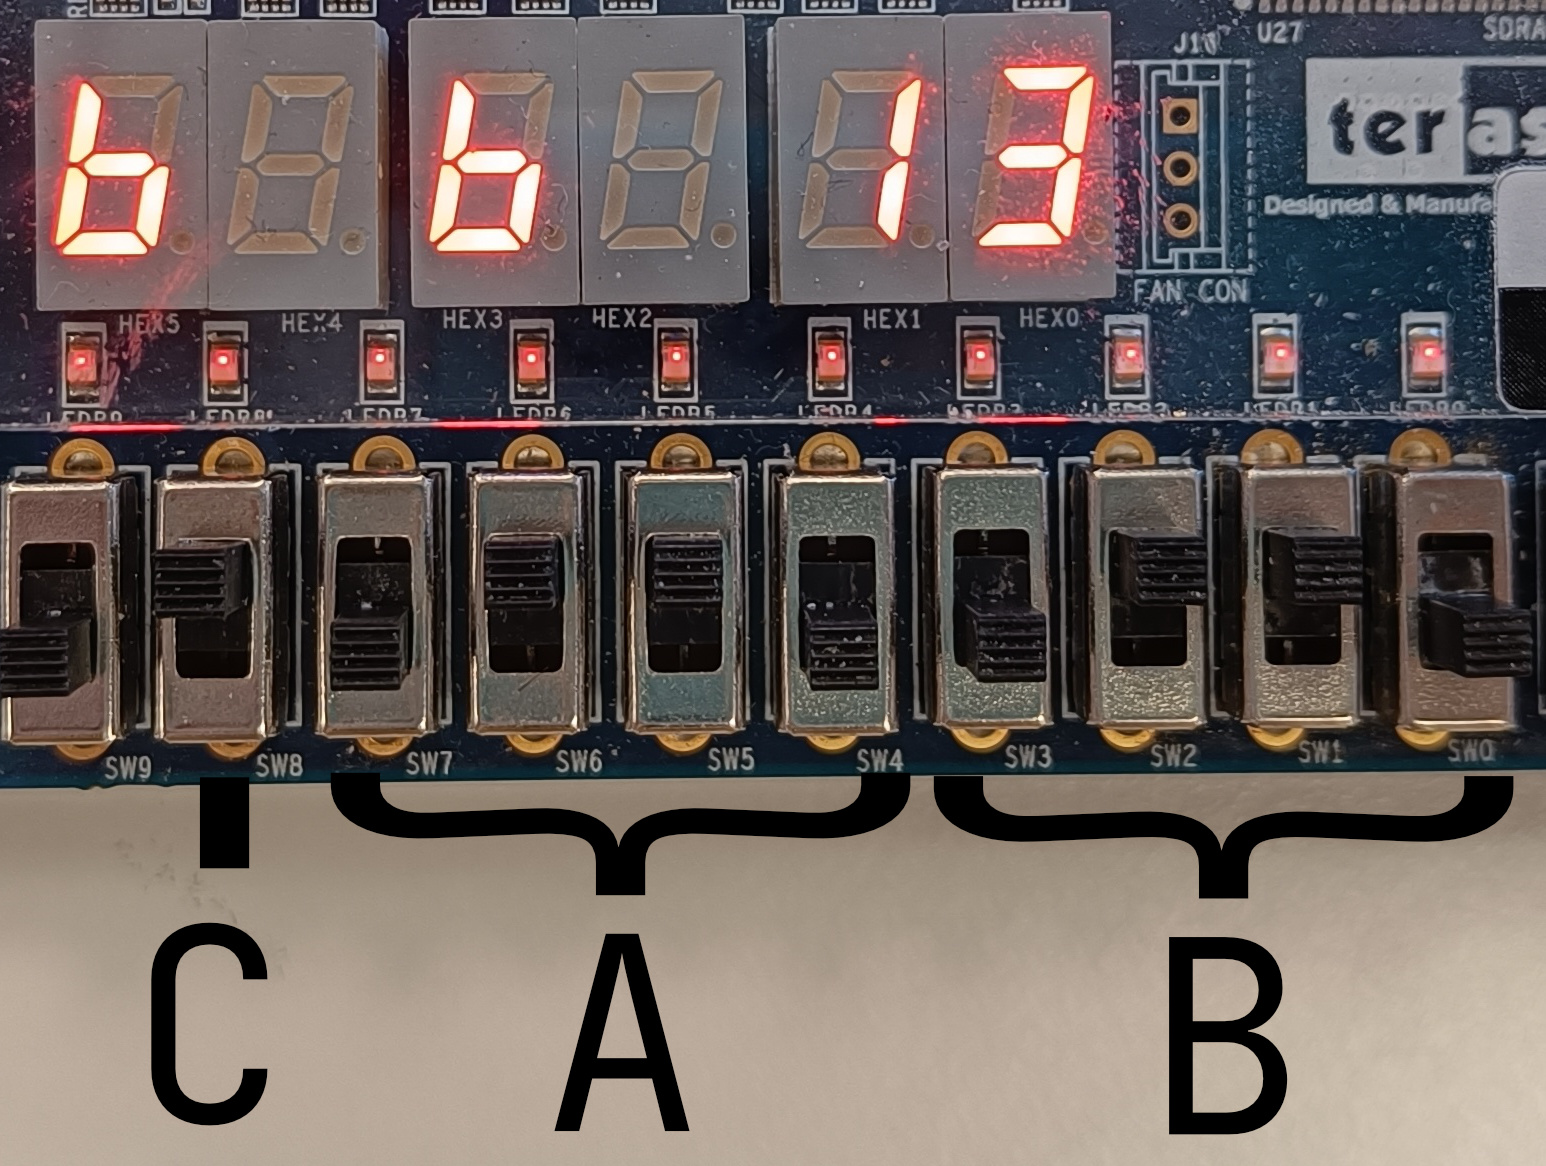
\includegraphics[width=1\textwidth]{Figures/Part5-1_6_6.jpg}
        \caption{1 + 6 + 6 = 13}
        \label{fig:T05pic4}
    \end{subfigure}
    \begin{subfigure}{0.4\textwidth}
        \centering
        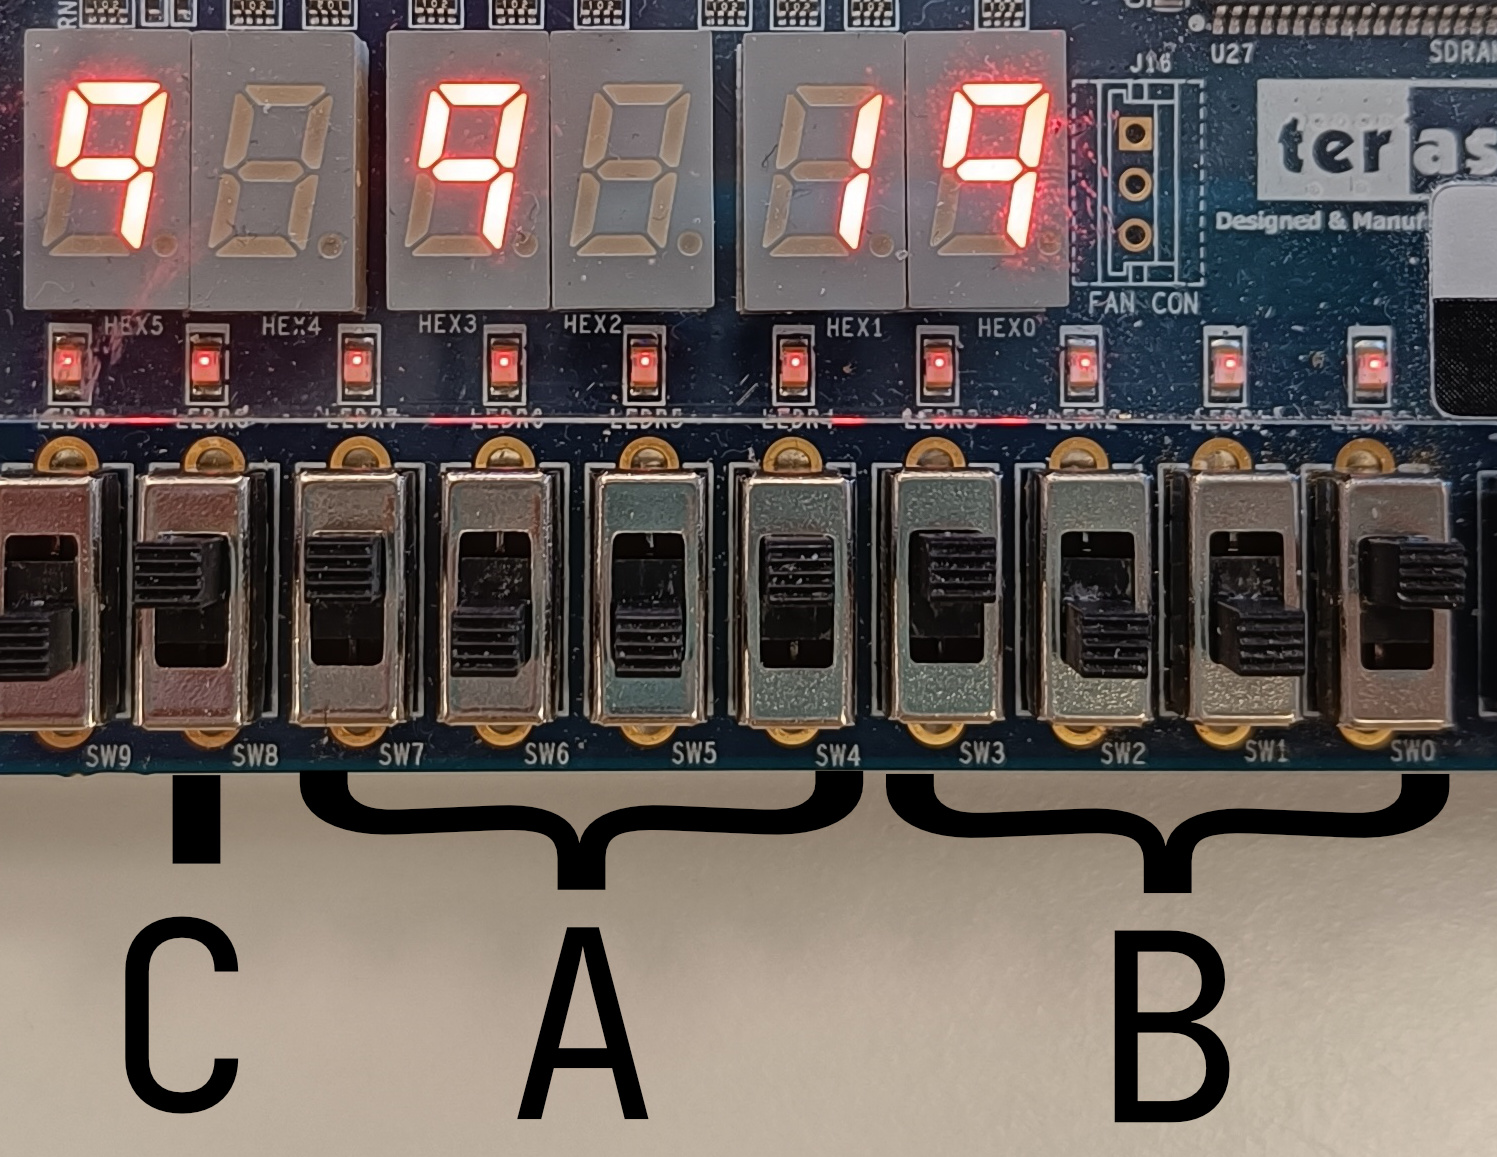
\includegraphics[width=1\textwidth]{Figures/Part5-1_9_9.jpg}
        \caption{1 + 9 + 9 = 19}
        \label{fig:T05pic5}
    \end{subfigure}
    \hfill
    \begin{subfigure}{0.4\textwidth}
        \centering
        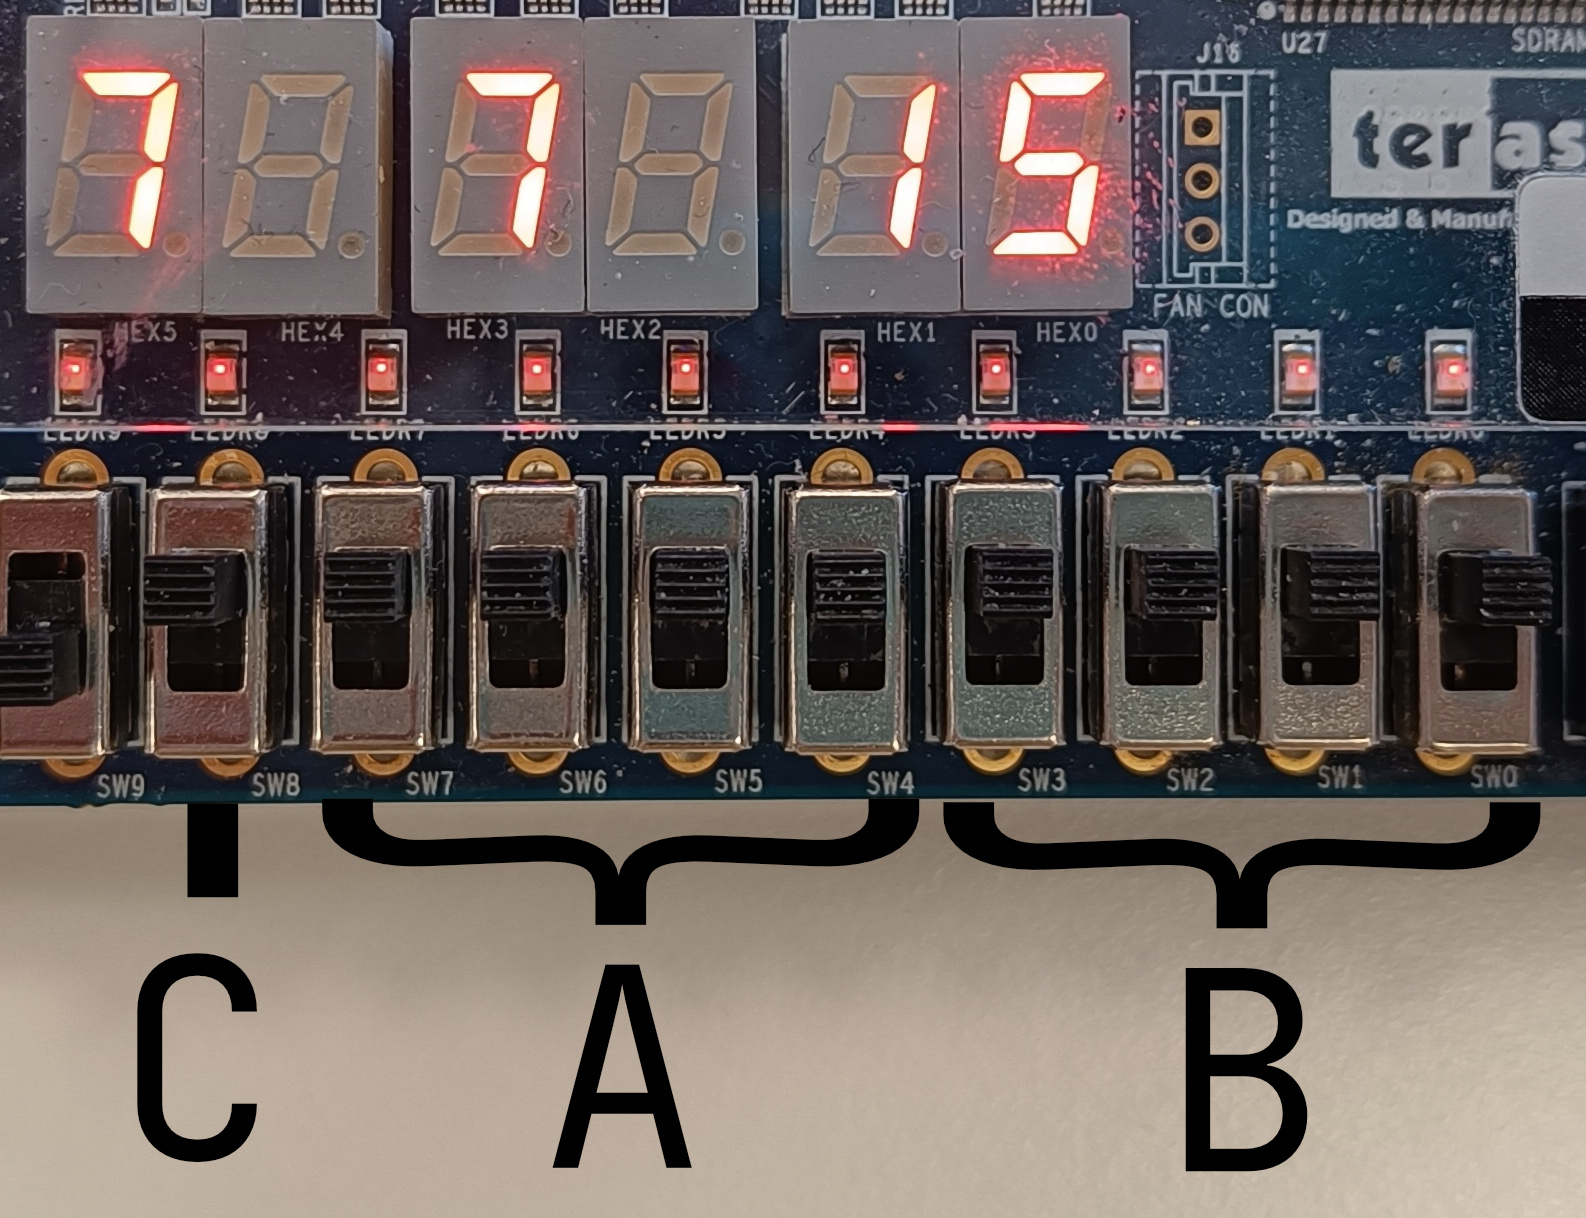
\includegraphics[width=1\textwidth]{Figures/Part5-1_15_15.jpg}
        \caption{Out of bounds}
        \label{fig:T05pic6}
    \end{subfigure}
    \figcaption{Test results}
    \label{fig:T05pic}
\end{figure}

\end{document}